\chapter{Implementação} \label{implementacao}

Neste capítulo iremos discutir a implementação das várias soluções descritas no capítulo \ref{capituloSolucoes}. Para tal há que fazer a distinção entre as duas vertentes da plataforma \gls{clav}:

\begin{itemize}
    \item \textbf{Frontend}
    
    O frontend da plataforma \gls{clav} é baseado na linguagem \emph{TypeScript}, uma variante fortemente tipada da linguagem \emph{JavaScript}, sendo utilizado o framework \emph{Vue} para a criação das páginas e interfaces responsáveis pela interação com o utilizador da plataforma.
    
    \item \textbf{Backend/API de dados}
    
    O backend da plataforma \gls{clav} foi desenvolvido em \emph{Node.JS}, utilizando uma \gls{api} REST para comunicação com o frontend. Este utiliza duas base de dados, cada uma com funções distintas na plataforma:
    
    \begin{itemize}
        \item \textbf{MongoDB}
        
        A base de dados não relacional, implementada em \emph{MongoDB} é responsável pelo armazenamento de informação relativa aos utilizadores, chaves \gls{api}, métricas entre outros.
        
        \item \textbf{GraphDB}
        
        A base de dados em grafos, implementada em \emph{GraphDB} é responsável pelo armazenamento de informação relativa às entidades, legislações, bem como a Lista Consolidada. Devido a se usar uma base de dados em grafos, esta permite cruzar informação de forma extremamente rápida e com pouco impacto no tempo de execução das queries, permitindo assim uma solução flexível, capaz de responder a pedidos específicos de forma rápida.
    \end{itemize}
\end{itemize}

Esta decisão de separar o frontend e backend cinge o primeiro a um papel de simples interface com o utilizador, devoluto de qualquer "lógica" aplicacional, ou seja, incapaz de realizar alterações em base de dados ou realizar pedidos à \gls{api}. 

Para obter tais informações, tem de comunicar com o backend, realizando pedidos conforme necessário, processando a resposta dada de modo a interagir com o utilizador. 

\vspace{5mm}
\begin{figure}[h!]
    \centering
    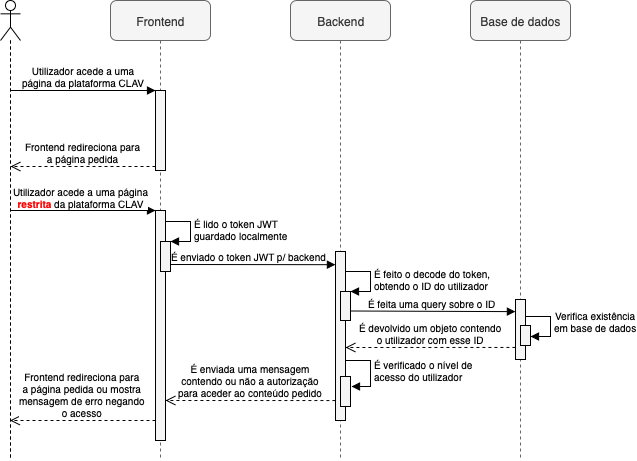
\includegraphics[width=\textwidth]{img/diagramas/sequencia/DiagramasSequencia.png}
    \caption{Diagrama de sequência ilustrativo da comunicação entre frontend e backend na plataforma \gls{clav}.}
    \label{fig:diagramaPaginaRestrita}
\end{figure}

Como podemos ver no diagrama de sequência da figura \ref{fig:diagramaPaginaRestrita}, o frontend serve apenas para interação com o utilizador, sendo que grande porção da lógica aplicacional ocorre no backend, que após terminar a query ou pedido em questão, retorna para o frontend mensagens de sucesso, erro, etc.

Toda e qualquer tarefa, quer seja de registo, login, acesso a informação sobre uma entidade, etc, é realizada sobre uma \gls{api} desenvolvida especificamente para o frontend e backend comunicarem entre si de forma independente e totalmente modular, permitindo correr em servidores diferentes.

\cleardoublepage
\section{Encriptação de informação sensível} \label{encryption}

De modo a solucionar os problemas referidos na secção \ref{vulnerabilidades}, foi necessário proceder ao desenvolvimento de uma função criptográfica que não só solucionasse o problema relacionado com ataques via \emph{rainbow tables}, mas também fosse capaz de acompanhar os avanços tecnológicos a nível computacional.

Para tal, Niels Provos e David Mazières desenvolveram a função de \emph{hashing} designada por \textbf{bcrypt}\cite{provos1999future}. Esta foi apresentada em 1999 na \gls{usenix}, sendo uma função baseada na cifra \emph{Blowfish}\footnote{Cifra assimétrica utilizada em criptografia.}, desenvolvia por Bruce Schneier e apresentada em 1993.

Além de incorporar um \emph{salt} para proteger contra ataques via \emph{rainbow tables}, esta foi desenvolvida para ser uma função adaptável, sendo que o número de iterações pode ser incrementado de modo a aumentar o número de ciclos máquina necessários para o cálculo do \emph{hash}. 

\begin{algorithm}
    \caption{Pseudo código do algoritmo \emph{bcrypt}.}
    \begin{algorithmic}[1]
        \Function{bcrypt}{cost, salt, pwd}
        \State $state\gets EksBlowfishSetup(cost,salt,key)$
        \State $ctext\gets OrpheanBeholderScryDoubt$
        \State \textbf{repeat}(64)
        \State \indent $ctext\gets EncryptECB(state, ctex)$
        \State \textbf{return} Concatenate(cost, salt, ctext)
    \EndFunction
    \end{algorithmic}
\end{algorithm}

Através do pseudo código acima descrito, é possível verificar que o algoritmo \emph{bcrypt} devolve uma string composta pelo custo, \emph{salt} e o hash da password.

Utilizando como exemplo a string "octavio" com um fator de custo 12, o algoritmo \emph{bcrypt} retorna o seguinte:

\begin{center}
    \textbf{\textcolor{red}{\$2y\$}\textcolor{green}{12\$}\textcolor{blue}{au1FX9q7Ju67N3INnoBo3uYqKrkYRLPFH1}\textcolor{orange}{.ycZ4GU9qHuo6c2FaN6}}
\end{center} 

Esta string pode ser dividida em 4 secções:

\begin{itemize}
    \item Versão do \emph{bcrypt} utilizada (representada a vermelho).
    \item Fator de custo, valor entre 1 e 31 (representada a verde).
    \item String correspondente ao \emph{salt} (representada a azul).
    \item Password após \emph{hash} da mesma(representada a laranja).
\end{itemize}

A combinação destas duas técnicas faz com que, até à data de publicação desta pré-dissertação, o algoritmo \emph{bcrypt} ainda não tenha sido quebrado, sendo que se trata do algoritmo escolhido por sistemas operativos como o \emph{OpenBSD}\footnote{Distribuição Unix open-source \url{https://www.openbsd.org}} e \emph{SUSE Linux}\footnote{Distribuição Unix open-source desenvolvida para soluções enterprise \url{https://www.suse.com/}} para o \emph{hashing} das suas passwords.

Esta fama levou a que o \emph{bcrypt} seja considerado por muitos, o standard da indústria em termos de encriptação de passwords.

\subsection{Funcionamento do bcrypt}

De modo a proporcionar uma forma de aumentar o tempo computacional o algoritmo \emph{bcrypt}, Niels Provos e David Mazières basearam-se na cifra \emph{Blowfish} já existente, criando assim uma versão designada por \emph{Eksblowfish} (\textit{\textbf{Expensive key schedule} Blowfish}).

\begin{algorithm}
    \caption{Pseudo código do algoritmo \emph{EksBlowfish}.}
    \begin{algorithmic}[1]
        \Function{EksBlowfishSetup}{cost, salt, key}
        \State $state\gets InitState()$
        \State $state\gets ExpandKey(state, salt, key)$
        \State \textbf{repeat}($2^{cost}$)
        \State \indent $state\gets ExpandKey(state, 0, salt)$
        \State \indent $state\gets ExpandKey(state, 0, key)$
        \State \textbf{return} state
    \EndFunction
    \end{algorithmic}
\end{algorithm}

Esta alteração à cifra \emph{Blowfish} não foi feita com o intuito de a tornar criptograficamente mais forte, mas sim alterar a forma como a \emph{key} é calculada.

Tendo em consideração que a \emph{key} é um valor aleatório variável entre 1 e 72 bytes, inclusive, esta alteração torna o cálculo da \emph{key} demoroso a nível computacional (\textbf{Expensive}).

De modo a prolongar o tempo de execução desta função, é aplicada a expansão da \emph{key} $2^{cost}$ vezes. Esta alteração é a maior distinção entre o algoritmo \emph{Blowfish} original e o \emph{Eksblowfish}, sendo a causa do \emph{bcrypt} ser considerado um algoritmo adaptável.

\newpage
No gráfico seguinte, podemos ver uma relação entre o factor de custo e o tempo de execução do algoritmo \emph{bcrypt}\footnote{Teste efetuado com processador Intel Core i7-4770K 4C/8T}.

\begin{center}
    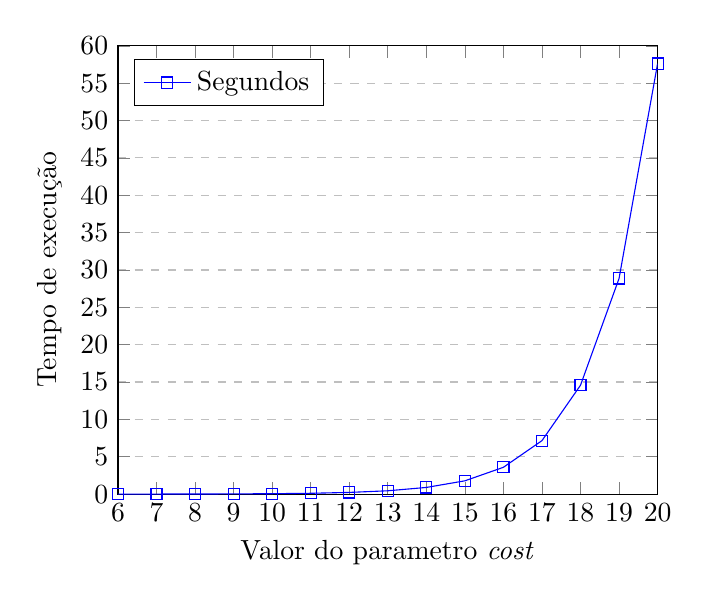
\begin{tikzpicture} 
        \begin{axis}[
            xlabel={Valor do parametro \emph{cost}},
            ylabel={Tempo de execução},
            xmin=6, xmax=20,
            ymin=0, ymax=60,
            xtick={6,7,8,9,10,11,12,13,14,15,16,17,18,19,20},
            ytick={0,5,10,15,20,25,30,35,40,45,50,55,60},
            legend pos=north west,
            ymajorgrids=true,
            grid style=dashed,
        ]
        \addplot[
            color=blue,
            mark=square,
            ]
            coordinates {
            (6,0.003622)(7,0.007590)(8,0.013918)(9,0.028723)(10,0.055023)(11,0.110837)(12,0.226982)(13,0.446507)(14,0.892617)(15,1.778647)(16,3.588397)(17,7.155973)(18,14.572114)(19,28.860461)(20,57.623139)
            };
            \legend{Segundos}
        \end{axis}
    \end{tikzpicture}
\end{center}

%\cleardoublepage
\subsection{bcrypt no mundo real}

Como foi mencionado nas secções prévias, um dos factos de o \emph{bcrypt} ainda ser utilizado deve-se não só à sua segurança, mas ao facto de acompanhar as evoluções tecnológicas a nível de processamento.

Quando foi originalmente lançado em 1999, devido ao tempo de execução do algoritmo \emph{bcrypt} ser adaptável, começou por ser utilizado um fator de custo de 6, pois este era o valor para o qual resultava um tempo de execução de aproximadamente 250ms (considerado por muitos o \emph{standard}).

Devido a enormes avanços tecnológicos, hoje em dia um fator de custo 6 na máquina previamente descrita leva a um tempo de execução de apenas 3.6ms, ou seja, aproximadamente 70 vezes menor do que em 1999.

Para combater esta crescente incessável de poder computacional, o fator de custo deve ser ajustado de acordo com o hardware atual, sendo que hoje em dia o fator de custo mais comum é de 12 a 14, o que nosso teste levou a um tempo de execução entre 226ms e 890ms.

De modo a exemplificar a importância do fator de custo, vamos imaginar o seguinte cenário:

\begin{itemize}
    \item Aplicação com 1000 utilizadores, cujas passwords estão contida num dos conjuntos em baixo especificados.
    \item Conjunto de passwords mais usadas:
    \begin{enumerate}
        \item 100 passwords.
        \item 1000 passwords.
        \item 10000 passwords.
    \end{enumerate}
    \item É permitido tentativas de autenticação ilimitadas, eliminando assim qualquer defesa contra ataques \emph{bruteforce}.
\end{itemize}

Quanto tempo demoraria a um atacante, com um processador idêntico ao descrito anteriormente, testar todas as passwords para os 1000 utilizadores?

\begin{center}
    \begin{tabular}{ |p{2.5cm}|p{3cm}|p{3cm}|p{3cm}|  }
        \hline
        \multicolumn{4}{|c|}{Tempo necessário para testar todas as passwords para os 1000 utilizadores.} \\
        \hline
        Fator de custo & 100 passwords & 1000 passwords & 10000 passwords\\
        \hline 
        6 & 6 minutos & 1 hora & 10 horas\\
        7 & 12 minutos & 2 horas & 21 horas\\
        8 & 23 minutos & 4 horas & 2 dias\\
        9 & 48 minutos & 8 horas & 3 dias\\
        10 & 92 minutos & 15 horas & 6 dias\\
        11 & 3 horas & 30 horas & 13 dias\\
        12 & 6 horas & 3 dias & 1 mês\\
        13 & 12 horas & 5 dias & 2 meses\\
        14 & 1 dia & 10 dias & 3 meses\\
        15 & 2 dias & 21 dias & 7 meses\\
        16 & 4 dias & 1 mês & 1 ano\\
        17 & 1 semana & 3 meses & 2 anos\\
        18 & 2 semanas & 6 meses & 5 anos\\
        19 & 1 mês & 11 meses & 9 anos\\
        20 & 2 meses & 2 anos & 18 anos\\
        \hline
    \end{tabular}
\captionof{table}{Tempo necessário para testar combinações de passwords para 1000 utilizadores.}\label{tab:bcrypt_bruteforce} 
\end{center}

Facilmente percebemos que fatores de custo como 10 são demasiado baixos para a atualidade, sendo imperativo a escolha de um fator de custo equilibrado. Outro facto a ter em consideração é este teste ter sido feito com um processador \emph{mainstream}, sendo que o mesmo se encontra 4 gerações atrasado em comparação com a atual 9ª geração de processadores Intel.

Outro problema que tem ganho tração nos últimos anos, é o aparecimento de soluções especializadas sobre a forma de \gls{gpu}, \gls{fpga}\cite{wiemer2014high}\cite{malvoni2014your} e \gls{asic}, capazes de poder computacional extremamente superior, quando comparados com o \gls{cpu} utilizado para os testes anteriores.

Um \gls{fpga} é um circuito integrado que tem a possibilidade de ser reprogramado através de \emph{bitstreams}, de modo a ser utilizado em aplicações diferentes, como por exemplo, cálculos de hash baseados no algoritmo SHA-1, SHA-256, etc. Enquanto que um \gls{asic}, embora também seja um circuito integrado, apenas consegue fazer uma função e não pode ser reprogramado, no entanto oferece performance muito superior a um \gls{fpga}.

Na tabela \ref{tab:bcrypt_hashrate} exploramos a performance em hashes por segundo (H/s) entre \gls{cpu}\footnote{\gls{cpu} fabricado pela Intel, desenvolvido na arquitetura \emph{Sandy Bridge}.}, \gls{gpu}\footnote{\gls{gpu} fabricada pela NVIDIA, desenvolvida na arquitetura \emph{Maxwell}.} e \gls{fpga}\footnote{Ambos os \gls{fpga} utilizados para comparação são desenvolvidos pela Xilinx.} relativamente ao algoritmo \emph{bcrypt}.

\begin{center}
    \begin{tabular}{ |p{1cm}|p{2.5cm}|p{2cm}|p{2cm}|p{1.75cm}|p{0.9cm}|  }
        \hline
        \multicolumn{6}{|c|}{Cálculo de hashes por segundo (H/s) em diverso hardware.} \\
        \hline
        Tipo & Modelo & Custo 6 & Custo 12 & Consumo & Preço\\
        \hline
        CPU & Xeon E3-1240 & 6210 H/s & 50 H/s& 300W & 262\$\\
        GPU & GTX 750Ti & 1920 H/s& 15 H/s& 300W & 120\$\\
        FPGA & zedboard & 6511 H/s & 51.95 H/s& 4.2W & 319\$\\
        FPGA & Virtex-7 & 51437 H/s& 410.4 H/s& 20W & 3495\$\\
        \hline
    \end{tabular}
\captionof{table}{Comparação entre hardware no cálculo de H/s, eficiência e custo.\cite{wiemer2014high}}\label{tab:bcrypt_hashrate} 
\end{center}

Mais uma vez é possível identificar outro um problema que não foi previamente considerado: como ajustar o fator de custo para este tipo de hardware especializado, como por exemplo \gls{fpga} e \gls{asic}?

Infelizmente a resposta é que este ajuste é deveras impossível. O simples aumento do fator de custo é impensável, pois iria implicar tempos exponenciais de computação em \gls{cpu} mainstream.

Felizmente, tal aplicação de hardware pare este efeito ainda não foi detetada no mundo real e não aparenta qualquer problema de momento.

\cleardoublepage
\section{Autenticação de utilizadores}
A autenticação e gestão de utilizadores é feita através da combinação do middleware\footnote{Middleware é um software que funciona como intermediário entre dois programas.} designado por \emph{Passport} e a base de dados não-relacional\footnote{Estilo de base de dados livres de esquema, capazes de maior escalabilidade que as base de dados tradicionais.} implementada em \emph{MongoDB}.

Devido à informação sensível que pode ser guardada na mesma, campos como a password são, naturalmente, encriptados recorrendo à técnica discutida na secção \ref{encryption}.

%\subsubsection{Passport}
O \emph{Passport} é um middleware de autenticação, desenvolvido para \emph{NodeJS}, com mais de 500 estratégias\footnote{Uma estratégia pode ser interpretado como um mecanismo único de autenticação.} diferentes de autenticação. Foi criado para solucionar um único problema: \textbf{autenticar pedidos}.

Devido à natureza do \emph{Passport}, este é extremamente fácil de implementar numa dada aplicação, devido ao seu forte encapsulamento e ao facto de delegar qualquer funcionalidade, que não seja a autenticação, para a aplicação.

Devido à natureza das aplicações Web modernas, a autenticação pode ser feita por diversas estratégias. As estratégias exploradas neste projeto recairam sobre a escolha mais "tradicional", uma autenticação local com campos para \emph{username} e \emph{password} e a autenticação com o auxílio da ferramenta Autenticação.Gov.

\begin{figure}[h!]
    \centering
    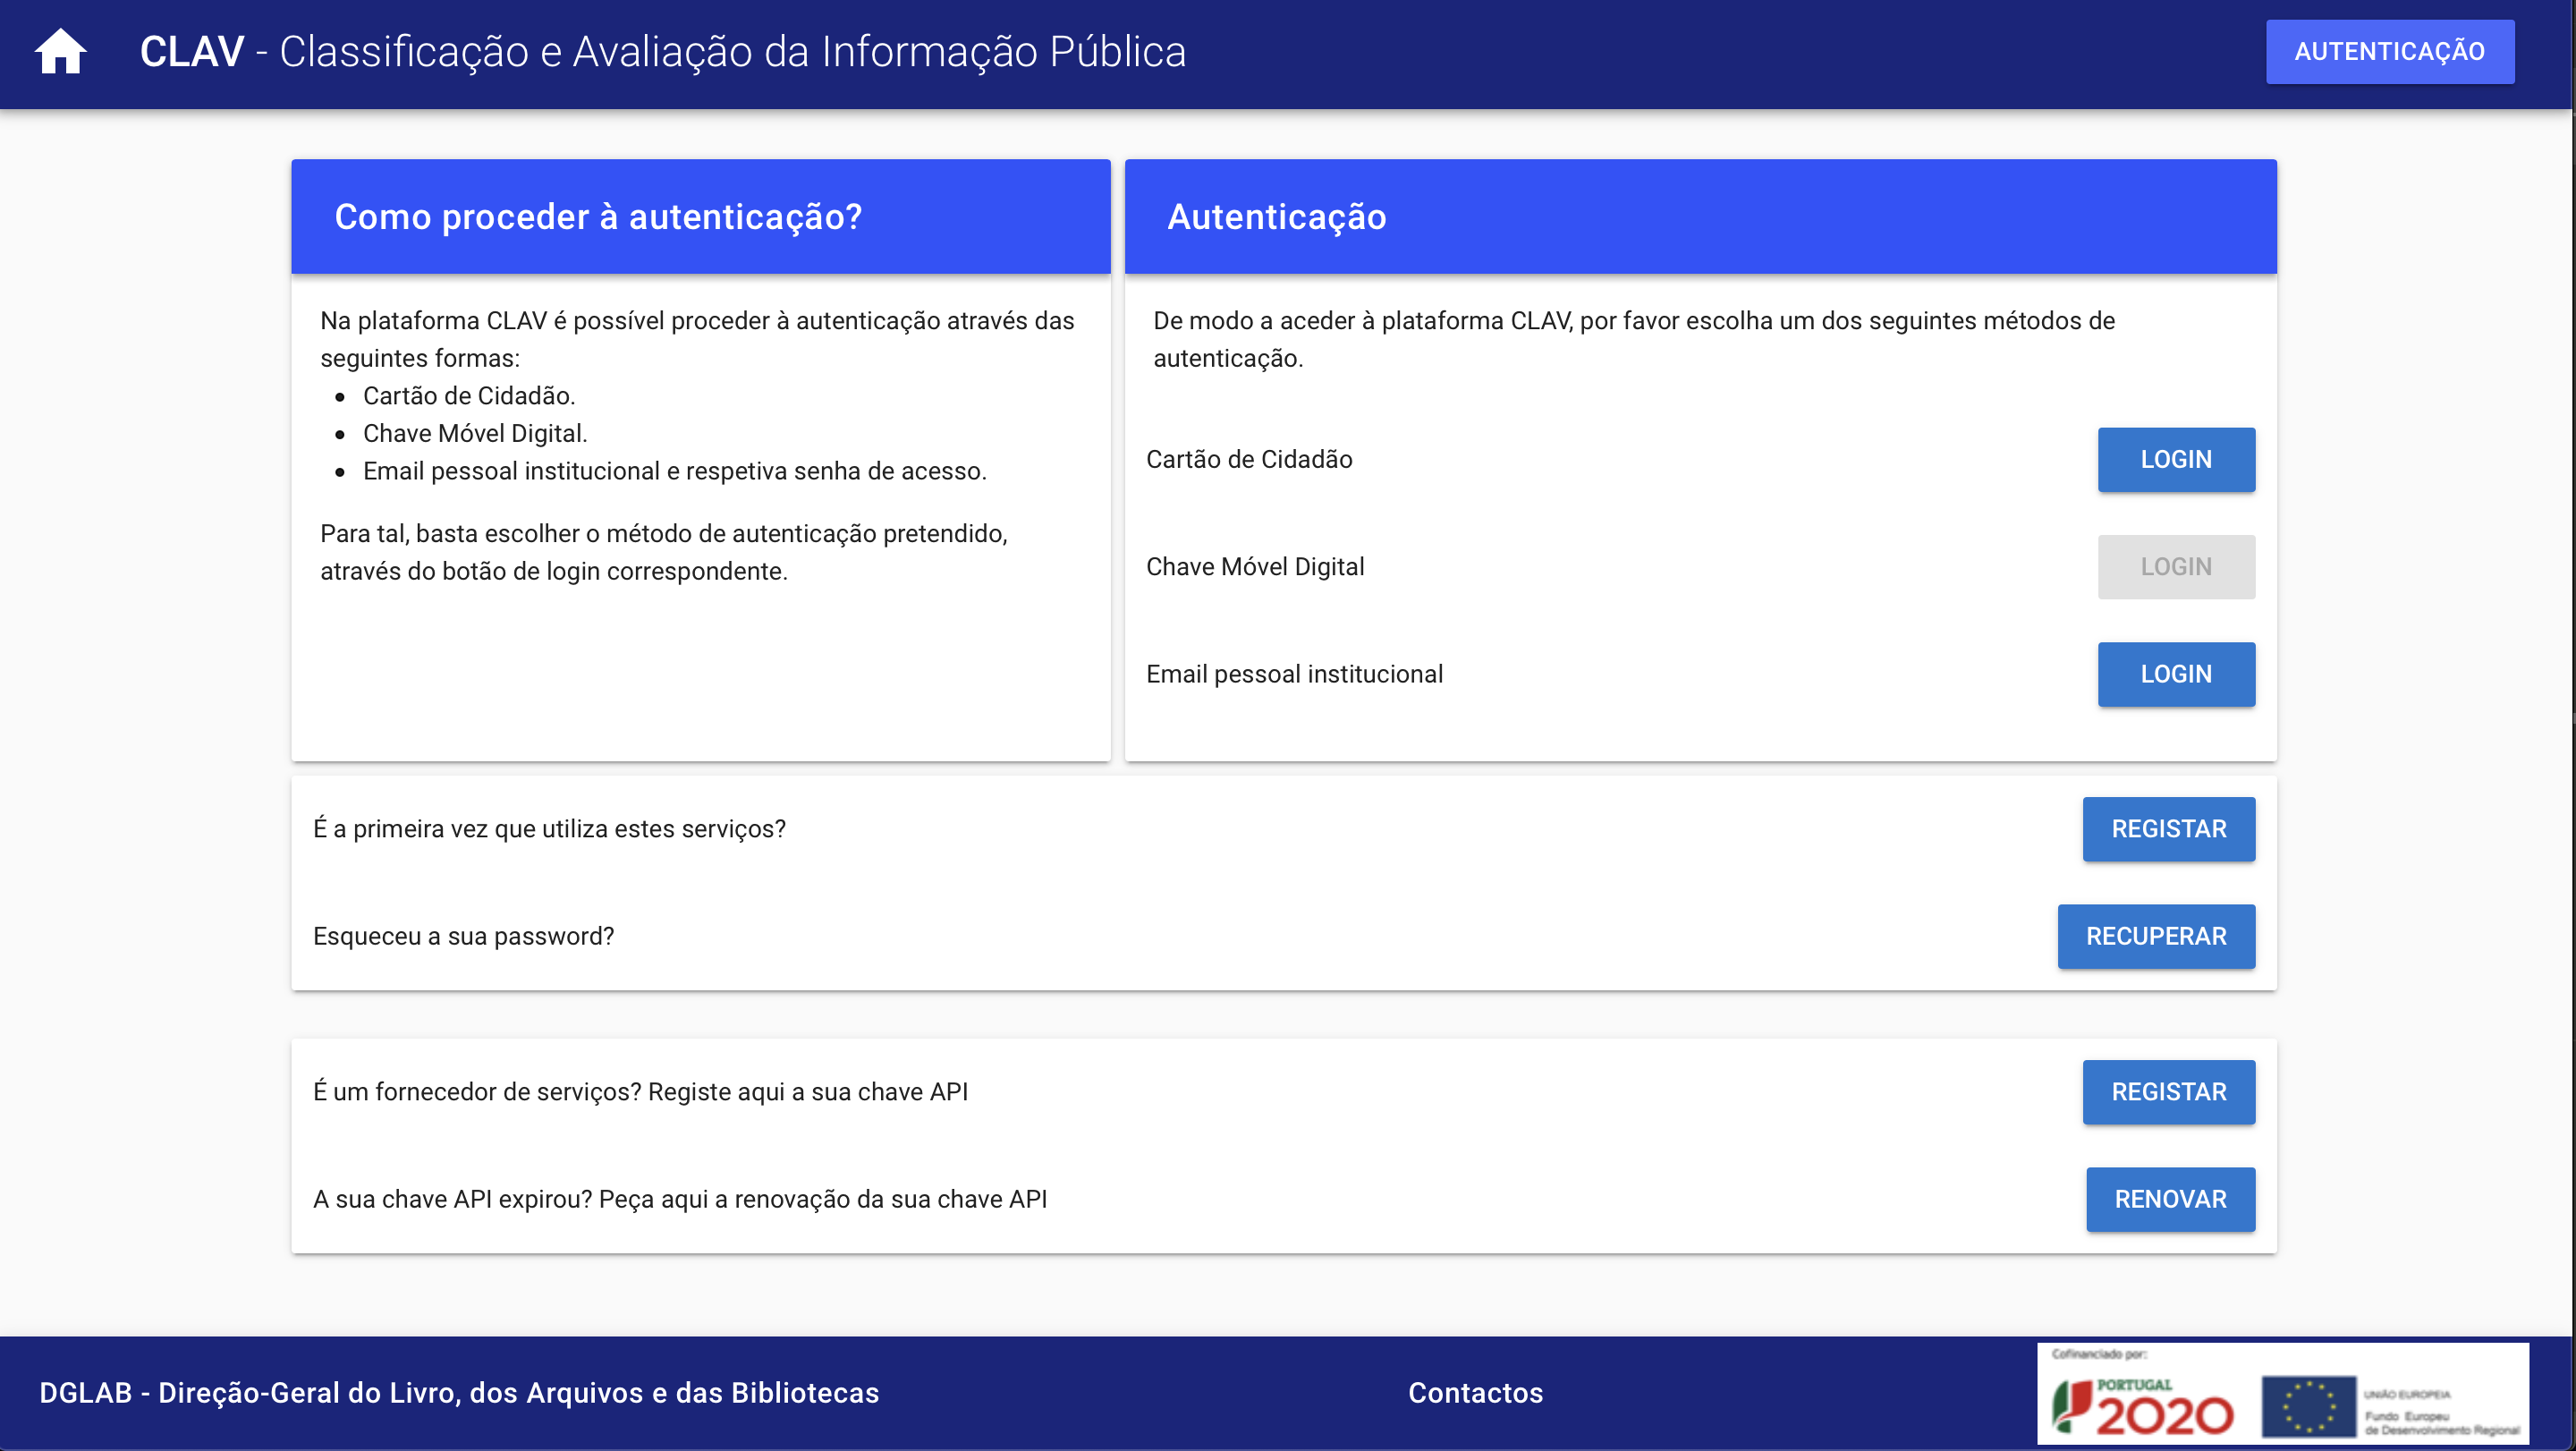
\includegraphics[width=\textwidth]{img/clav/paginaAuth.png}
    \caption{Página principal de autenticação na plataforma \gls{clav}.}
    \label{fig:paginaAutenticacao}
\end{figure}

Embora exista um aumento exponencial de implementações de autenticação baseadas em redes sociais, através de protocolos desenvolvidos em acordo com o \emph{OAuth}\footnote{Protocolo open-source que permite autenticação de forma standard e segura, entre aplicações desktop, web e mobile.}, tais como \emph{Google+} e \emph{Facebook}, foi decidido desde uma fase inicial que tais estratégias não seriam consideradas devido ao carácter profissional da plataforma.

Devido a cada aplicação possuir necessidades diferentes, o \emph{Passport} guarda cada estratégia de autenticação em módulos independentes, deixando assim a cargo do programador que estratégias empregar, sem criar dependências desnecessárias.

\subsection{Autenticação através de username e password}

Nesta secção iremos explorar a implementação da autenticação através de username a password, designada por autenticação local. Começaremos por analisar a página de registo, seguida de uma análise do diagrama de sequência da mesma, explicando em detalhe o processo de registo do início ao fim.

\subsubsection{Registo}

O registo local, através de username e password foi implementado com o objetivo de ser intuitivo e simples. 
%Para tal, foi criada uma página sucinta, onde são indicados os campos necessários para preenchimento.

\begin{figure}[h!]
    \centering
    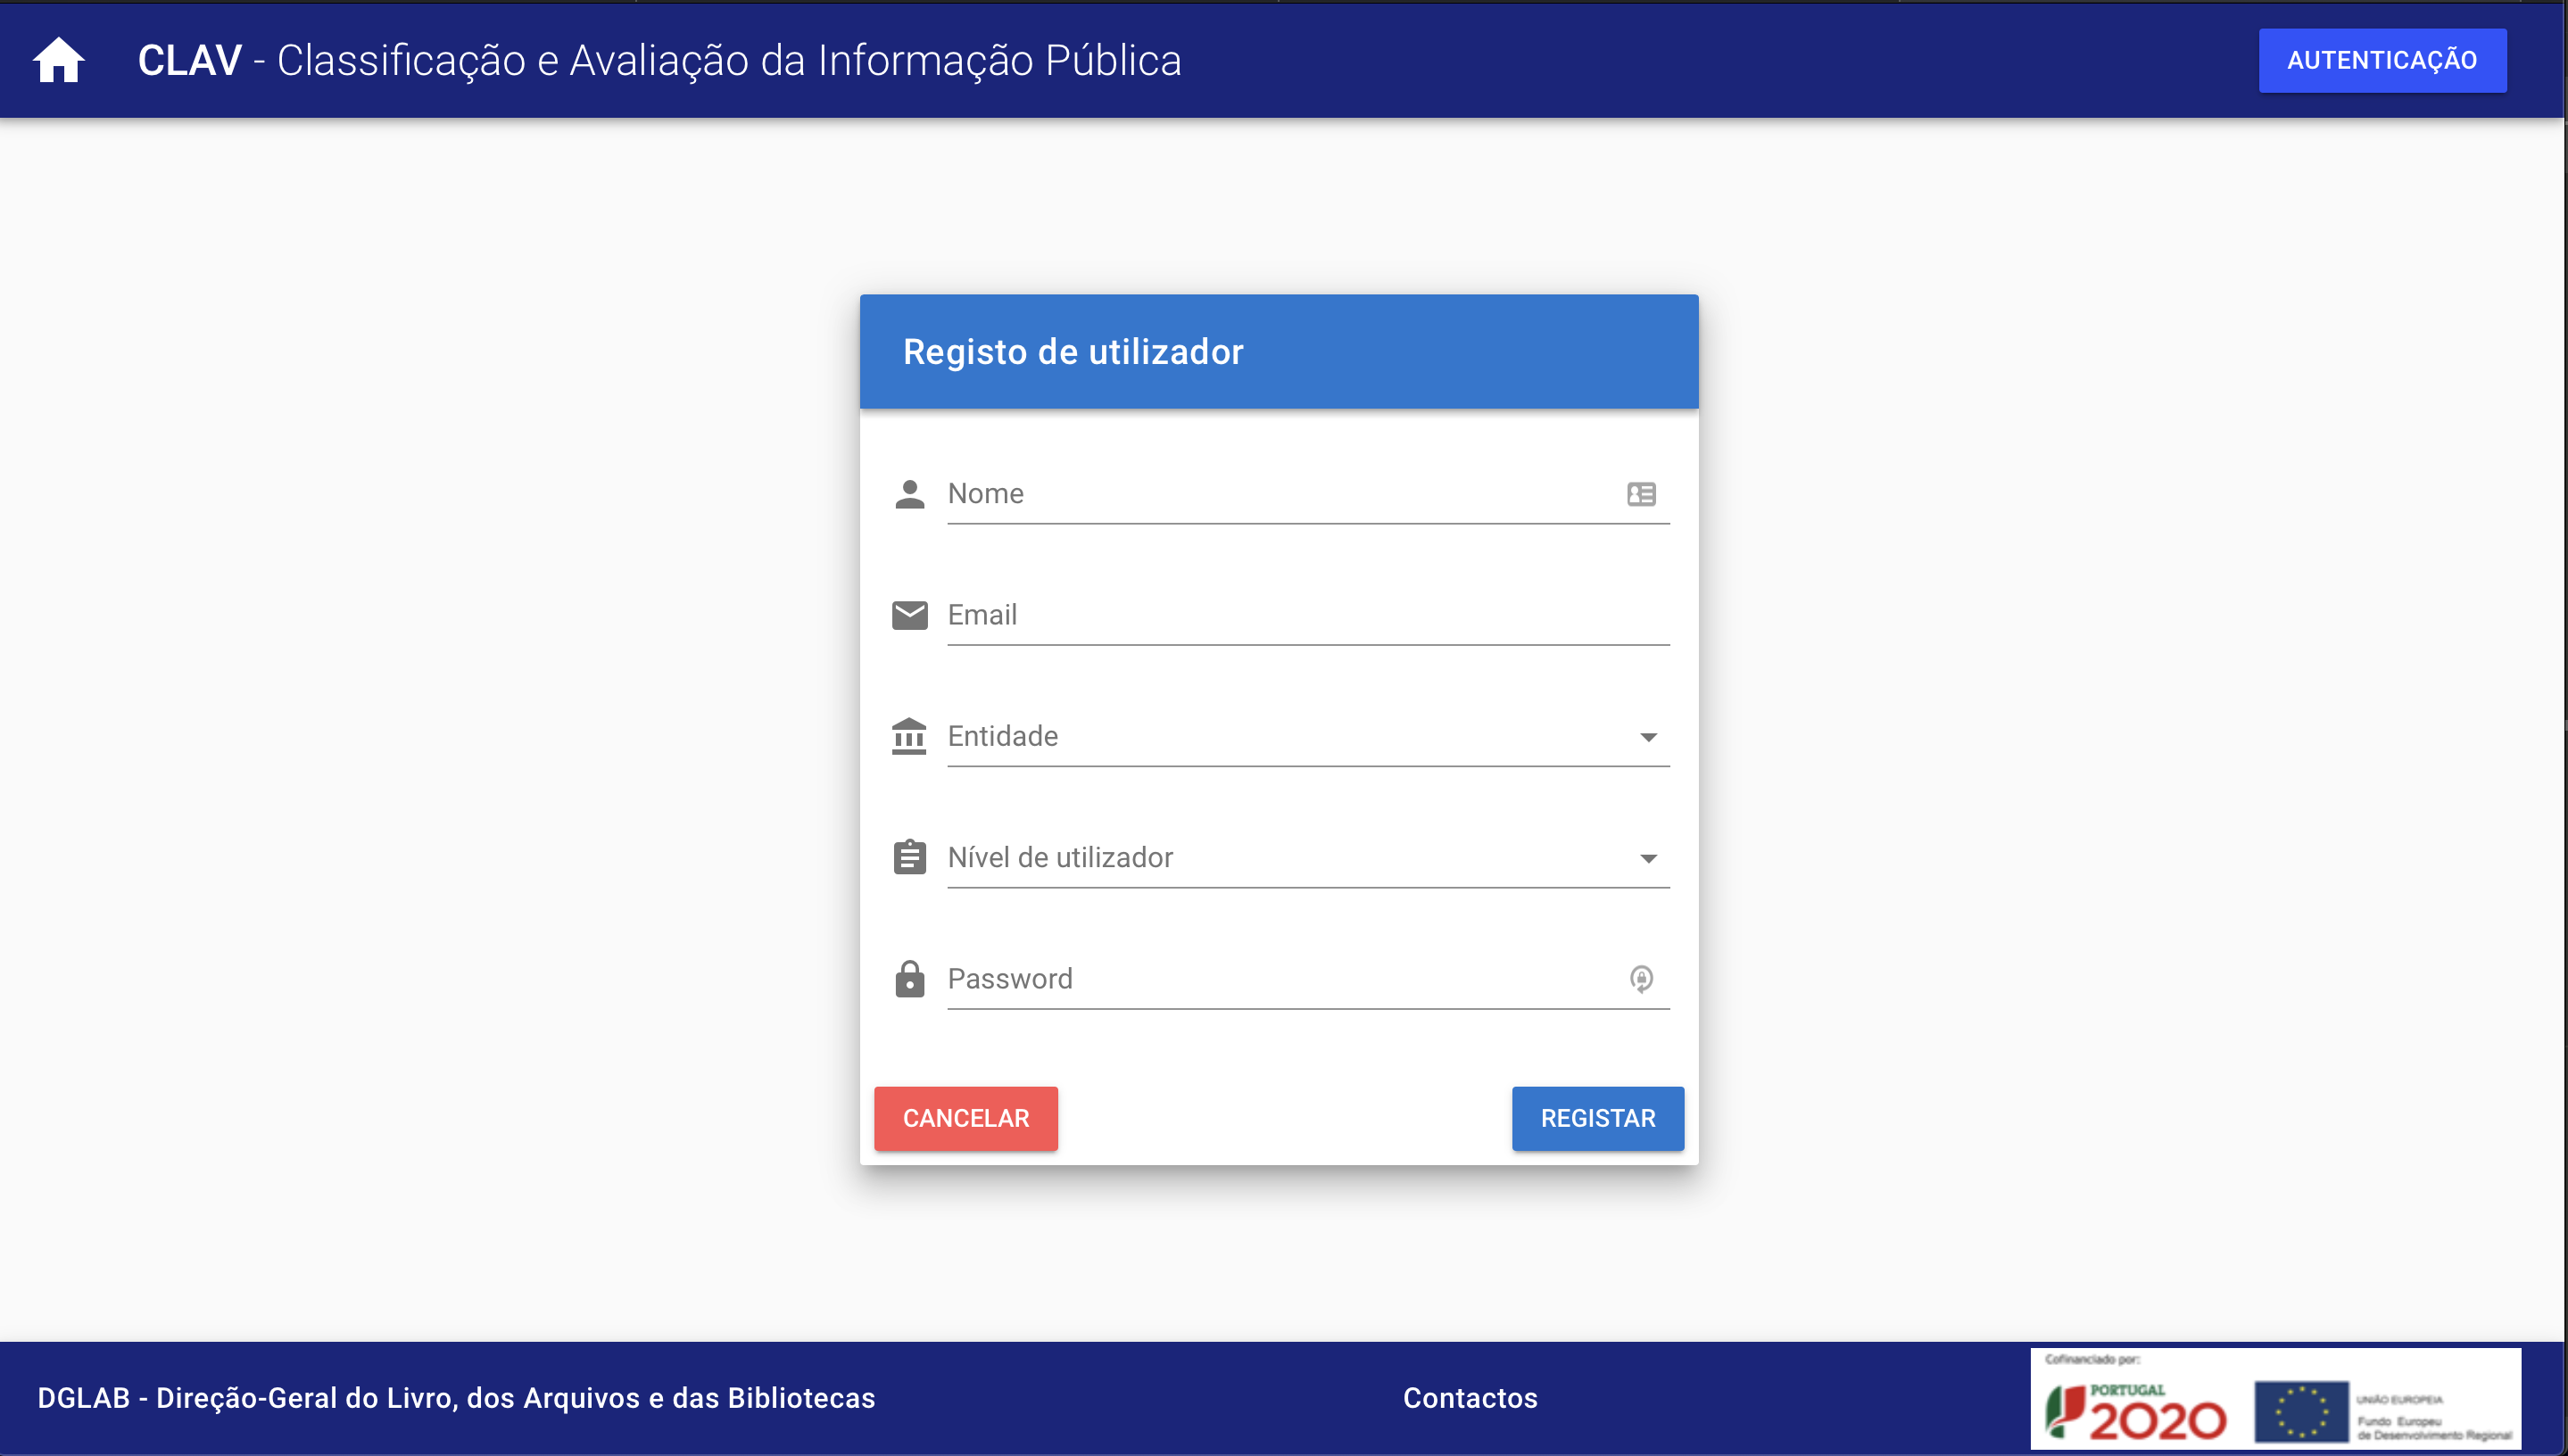
\includegraphics[width=\textwidth]{img/clav/authlocal/registo.png}
    \caption{Página de registo na plataforma \gls{clav}.}
    \label{fig:paginaRegistoLocal}
\end{figure}

Para tal é utilizado um form, onde é necessário o preenchimento da seguinte informação (como foi especificado na secção \ref{especificacaoAuthLocal}):
\begin{enumerate}
    \item Nome.
    \item Email.
    \item Entidade.
    \item Nível de utilizador.
    \item Password (encriptada através de \emph{bcrypt}, explicado na secção \ref{encryption}).
\end{enumerate}

Após submeter o pedido de registo pode ocorrer um dos seguintes cenários:

\begin{itemize}
    \item \textbf{Sucesso}
    
    Ocorre quando o utilizador fornece todos os dados necessários para o seu registo.
    
    \begin{figure}[h!]
        \centering
        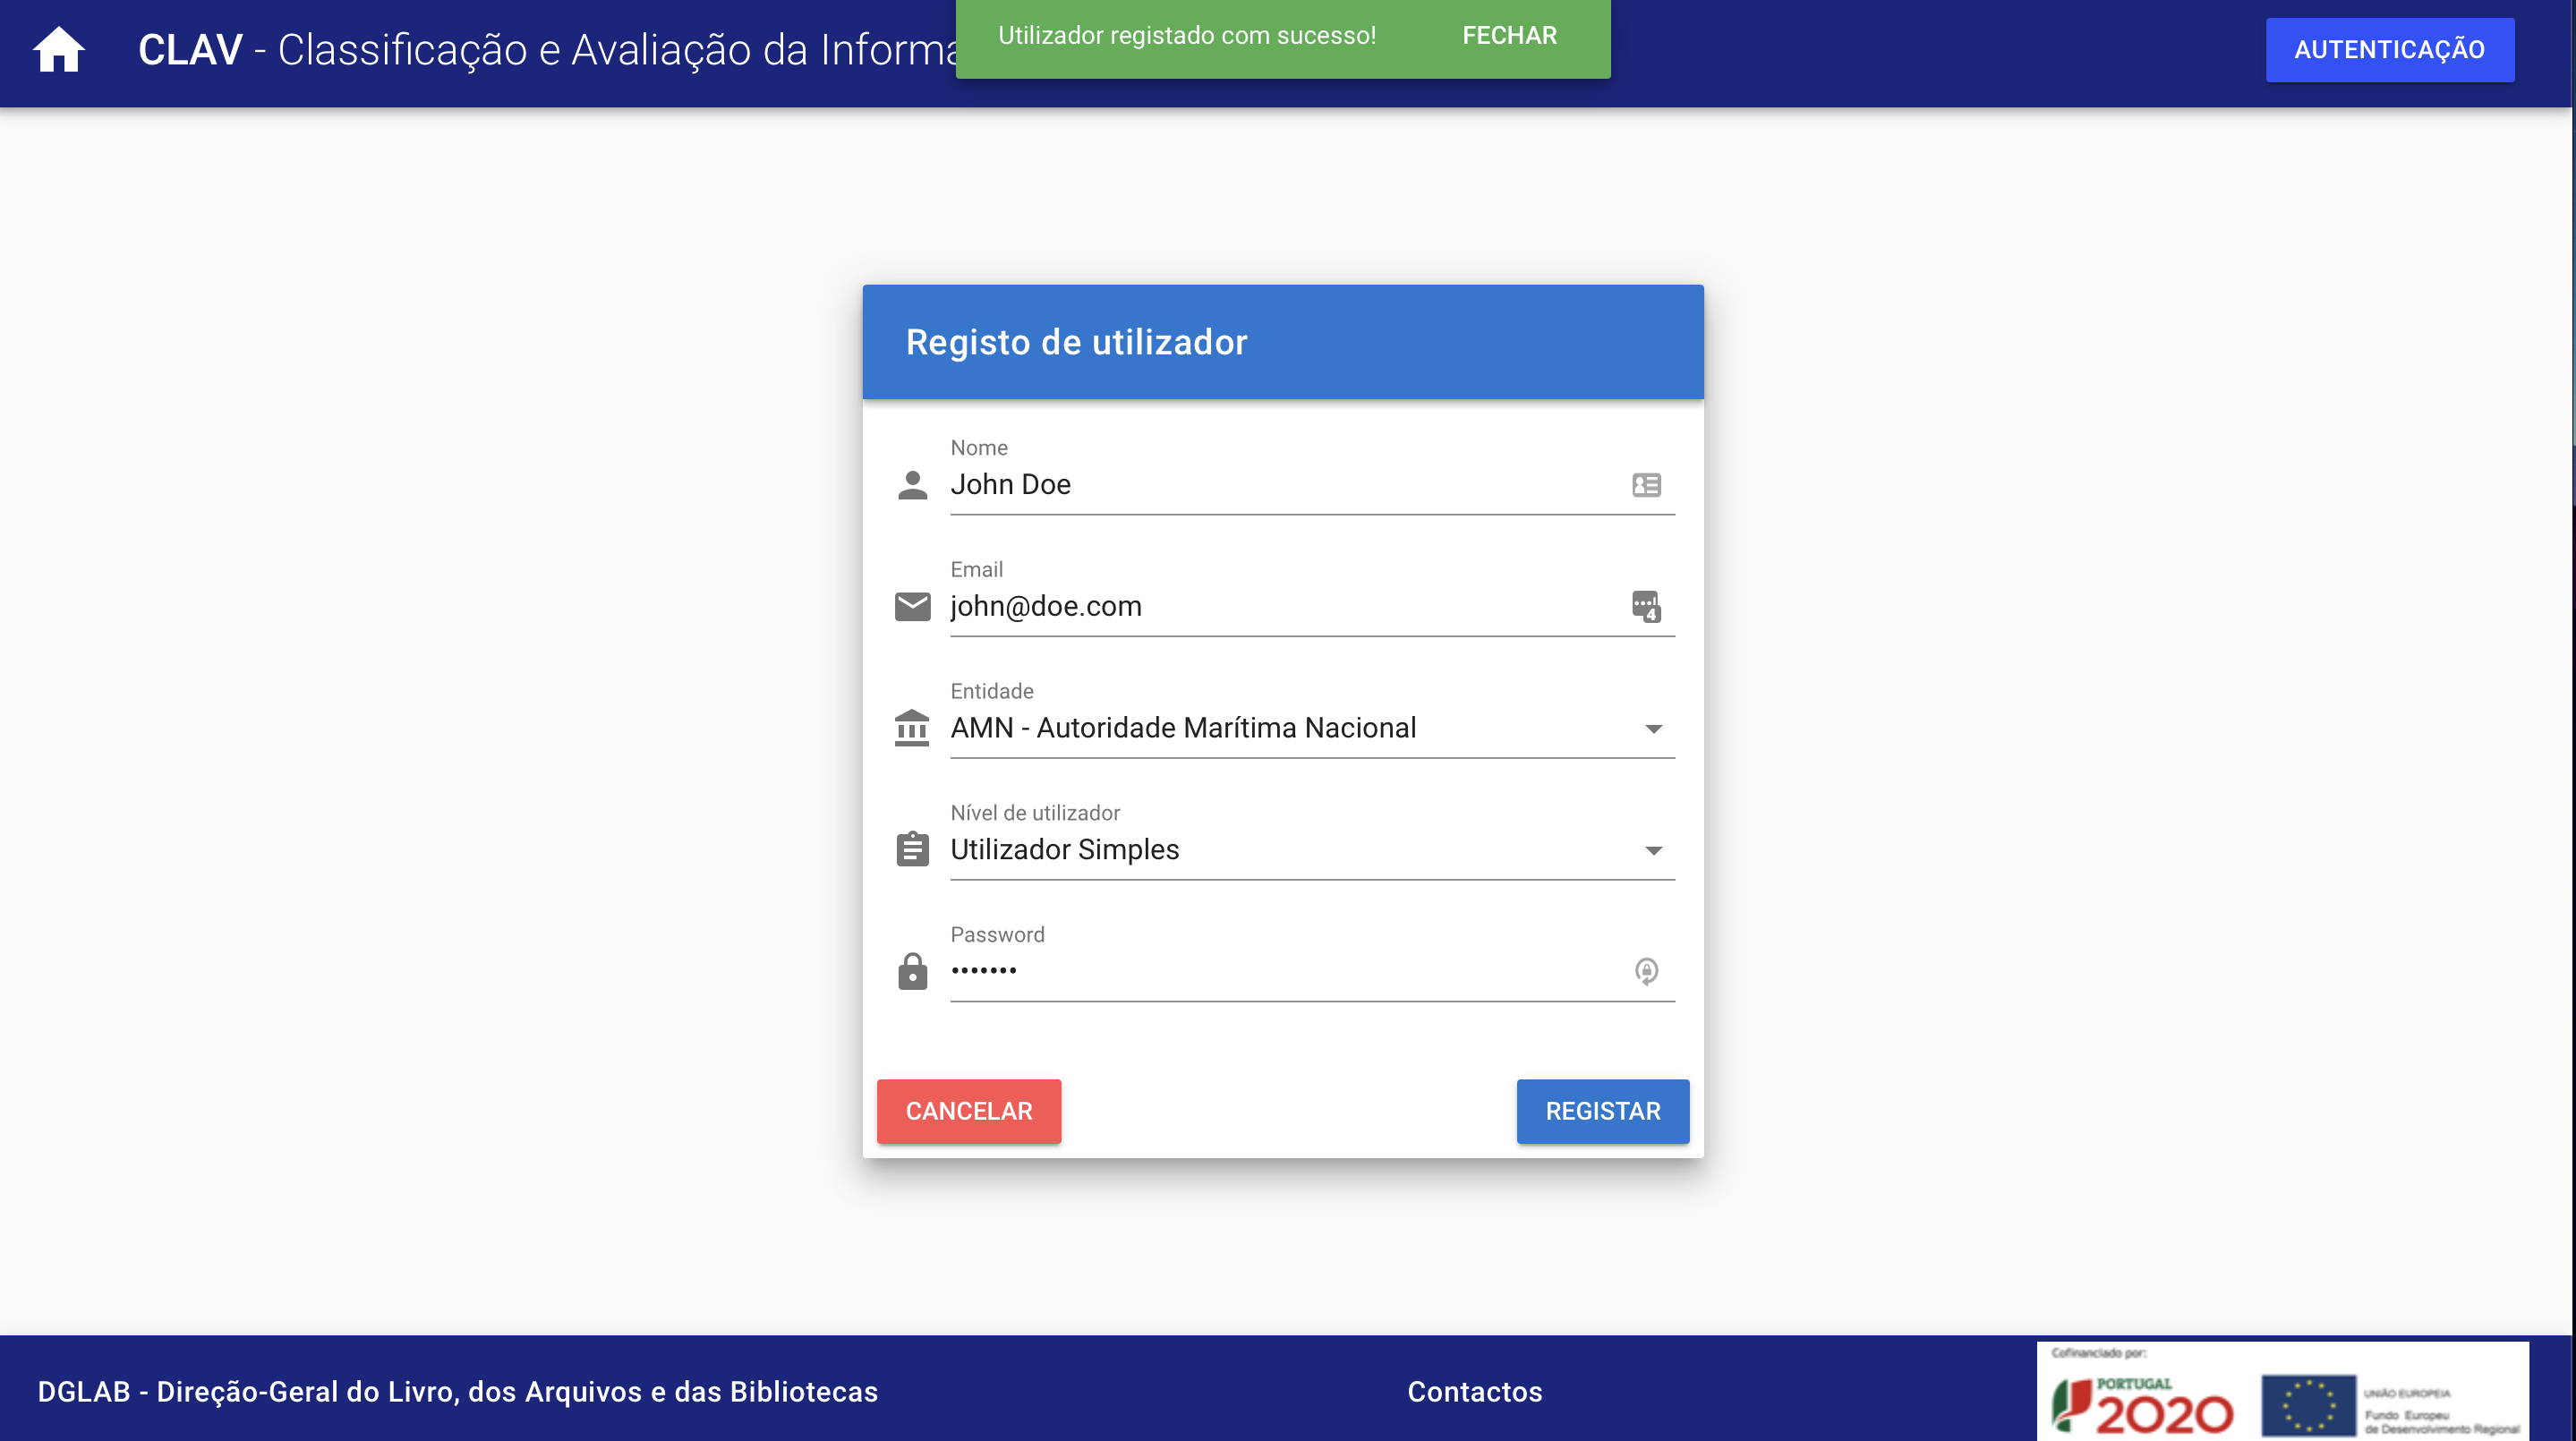
\includegraphics[width=\textwidth]{img/clav/authlocal/sucessoRegisto.png}
        \caption{Página quando ocorre um registo com sucesso na plataforma \gls{clav}.}
        \label{fig:registoSucesso}
    \end{figure}
    
    \item \textbf{Insucesso}
    
    \begin{itemize}
        \item \textbf{Dados insuficientes}
        
        Ocorre quando o utilizador não preencheu todos os campos necessários para o registo.
        
        \begin{figure}[h!]
            \centering
            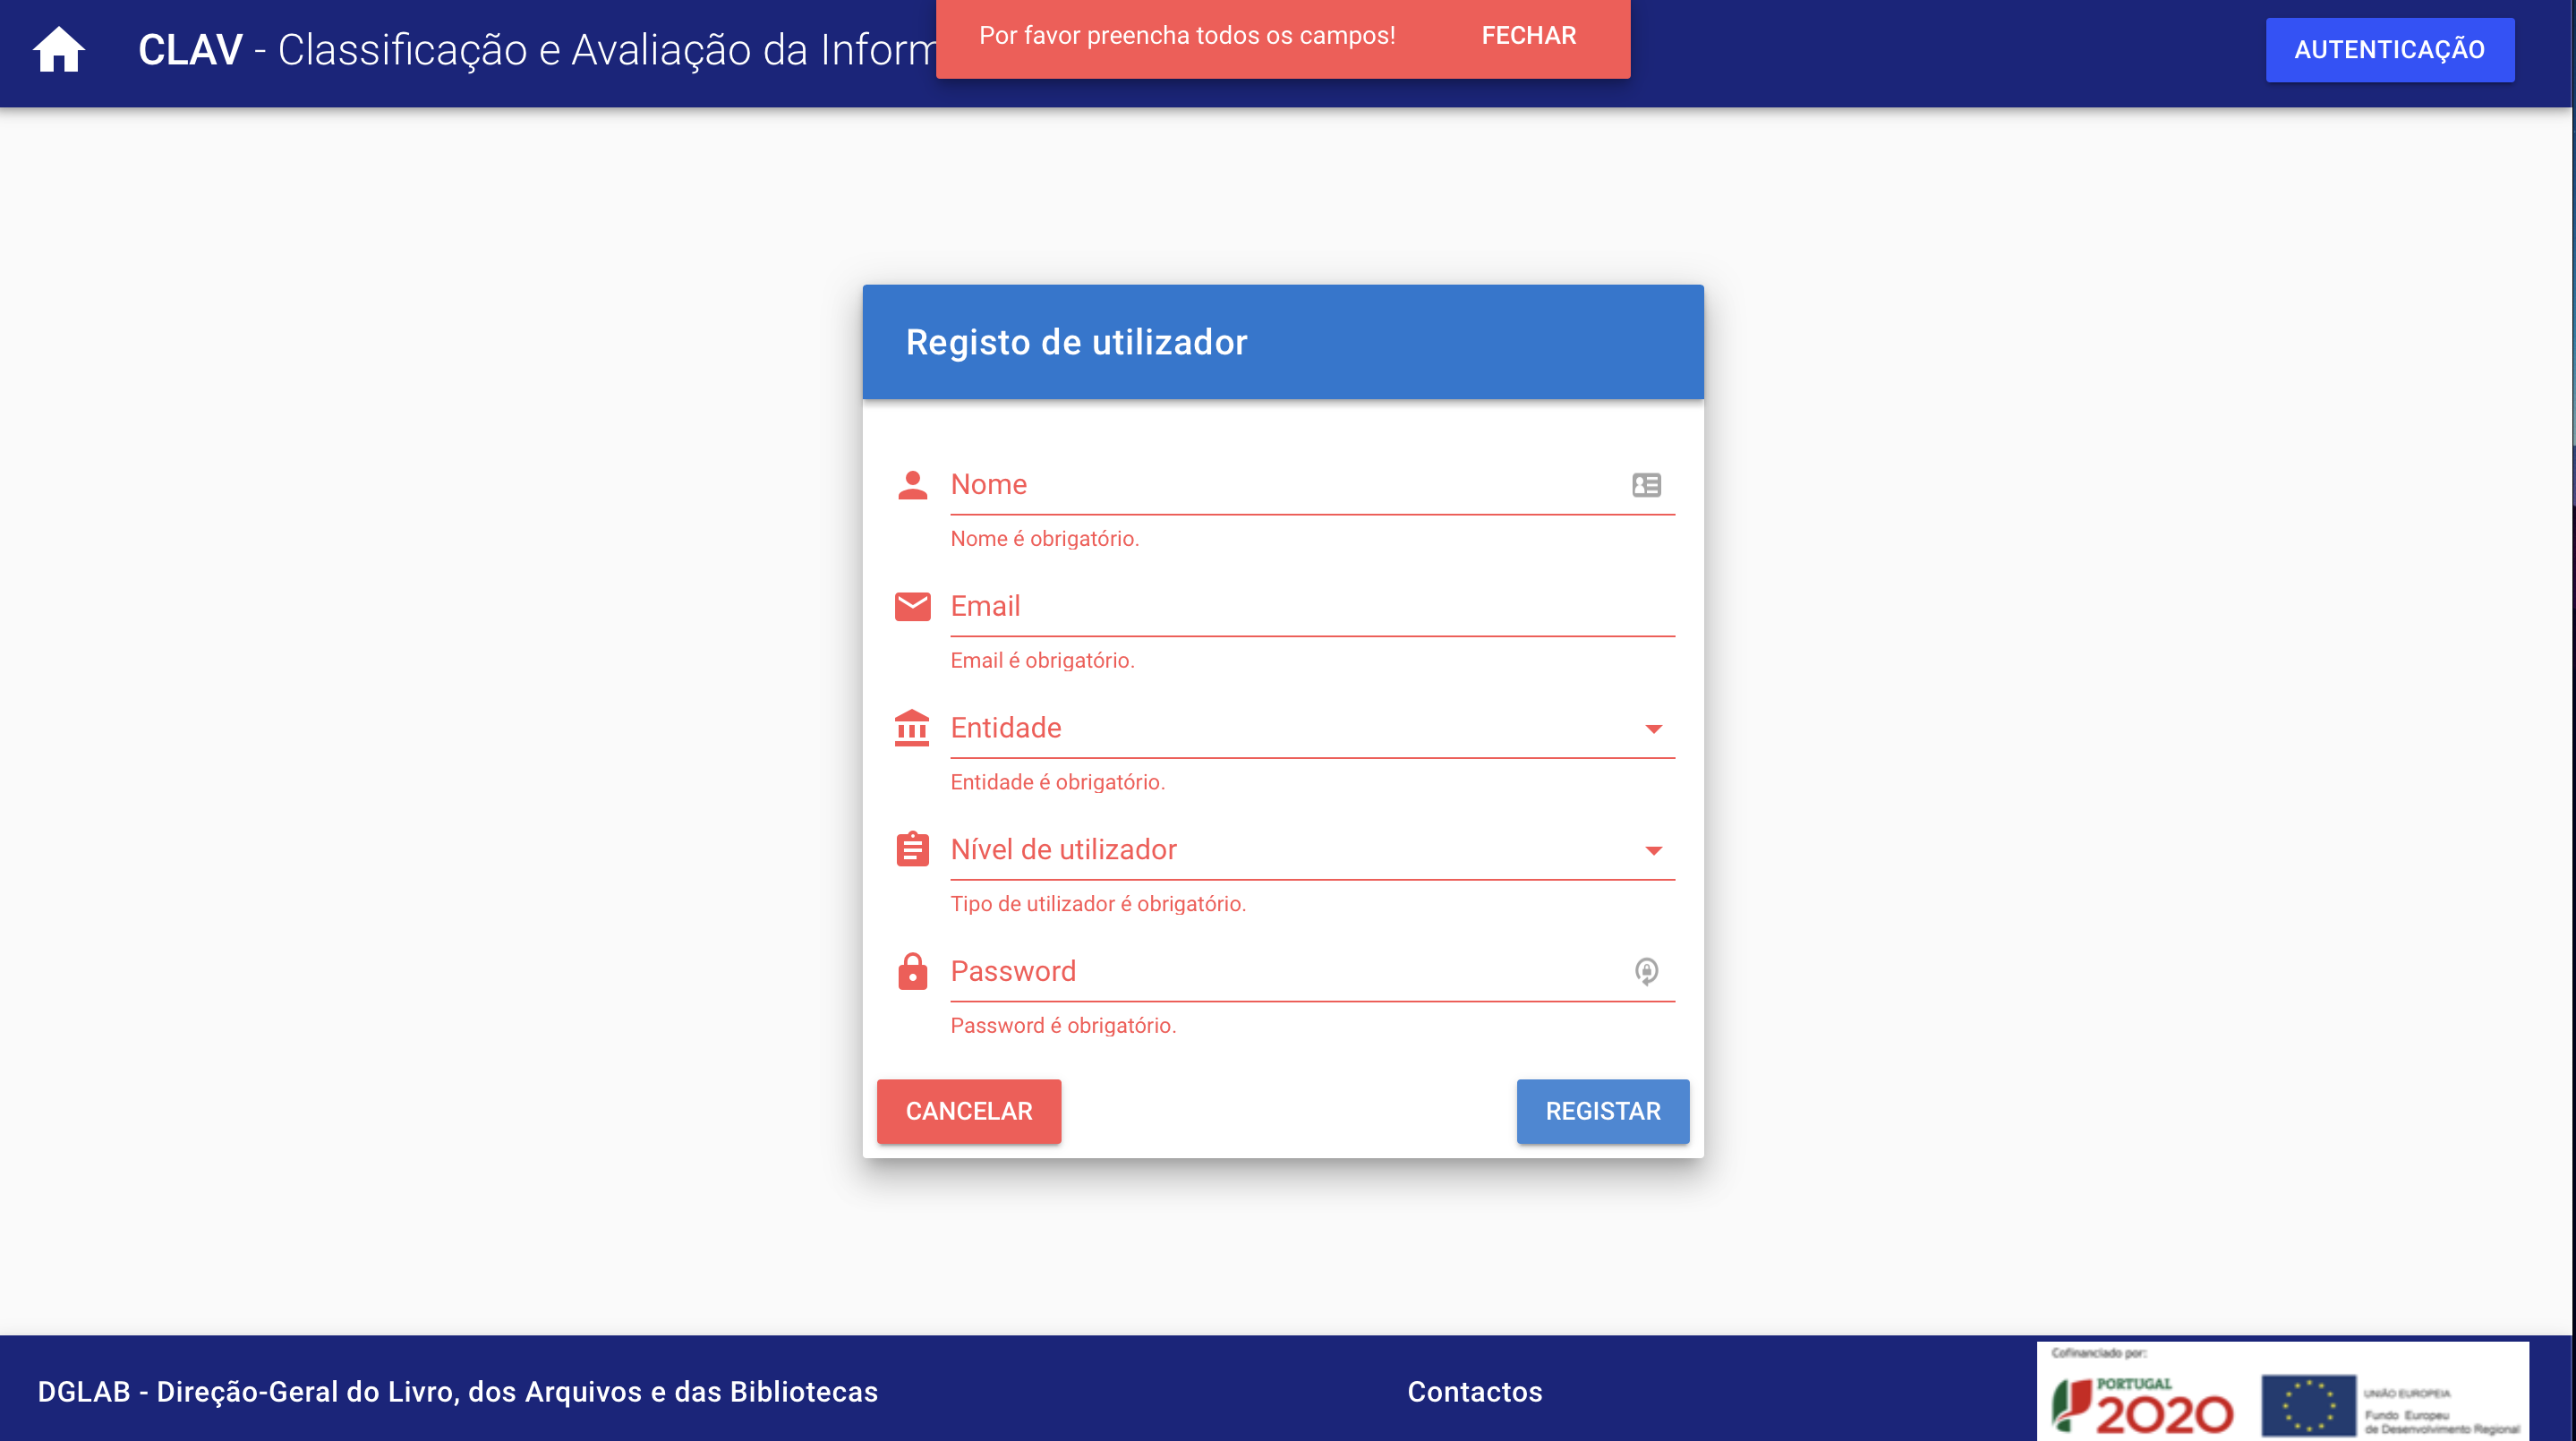
\includegraphics[width=\textwidth]{img/clav/authlocal/erroRegisto1.png}
            \caption{Página quando ocorre um erro de registo na plataforma \gls{clav}.}
            \label{fig:registoErro1}
        \end{figure}

        \vspace{5cm}
        \item \textbf{Email já registado}
        
        Ocorre quando o utilizador fornece um email já atribuido a outro utilizador.
        
        \begin{figure}[h!]
            \centering
            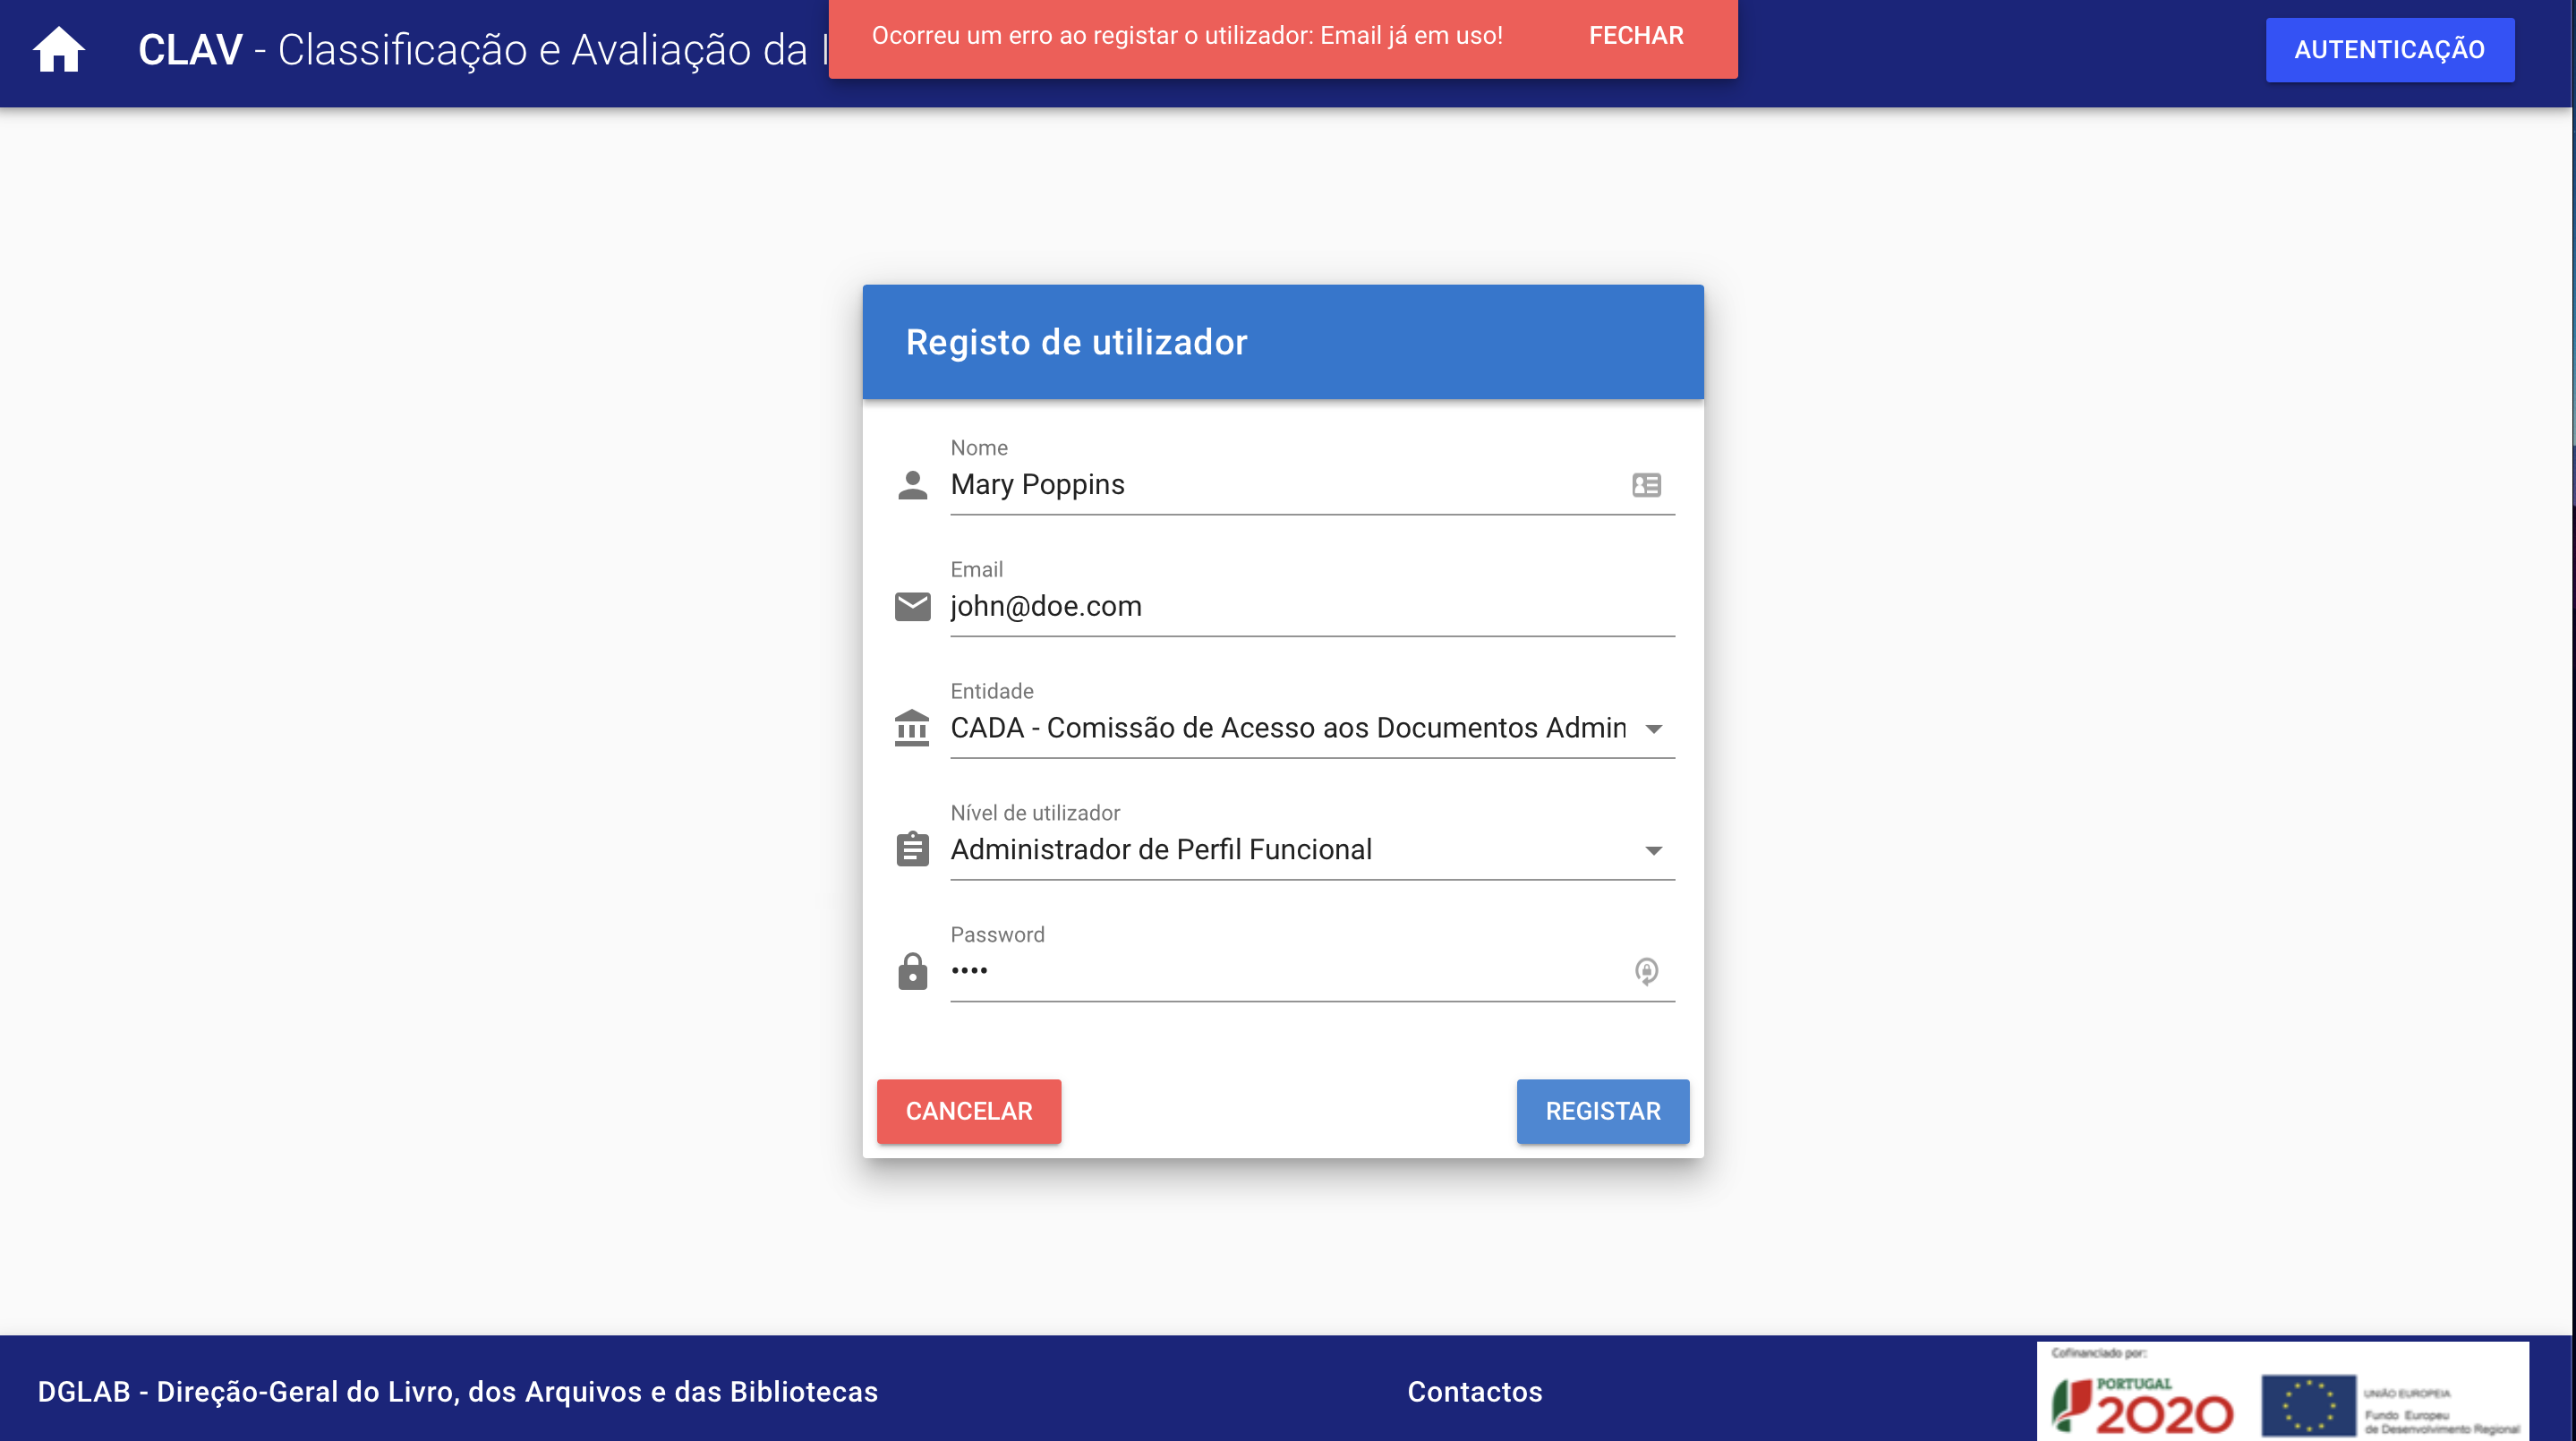
\includegraphics[width=\textwidth]{img/clav/authlocal/erroRegisto2.png}
            \caption{Página quando ocorre um erro de registo na plataforma \gls{clav}.}
            \label{fig:registoErro2}
        \end{figure}
        
    \end{itemize}
\end{itemize}

O comportamento da função de registo pode ser explicado pelo diagrama de sequência da figura \ref{fig:diagramaRegisto}.

\begin{figure}[h!]
    \centering
    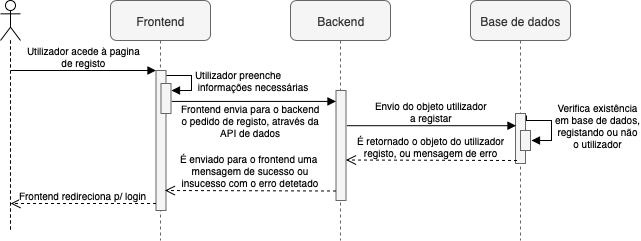
\includegraphics[width=\textwidth]{img/diagramas/sequencia/DiagramasSequencia-Registo.png}
    \caption{Diagrama de sequência correspondente ao processo de registo na plataforma \gls{clav}.}
    \label{fig:diagramaRegisto}
\end{figure}

\vspace{-4mm}
\subsubsection{Login}

Tendo em consideração a página de registo local, foi implementada uma solução similar, apenas com os campos necessários para login, ou seja, email e password.

\begin{figure}[h!]
    \centering
    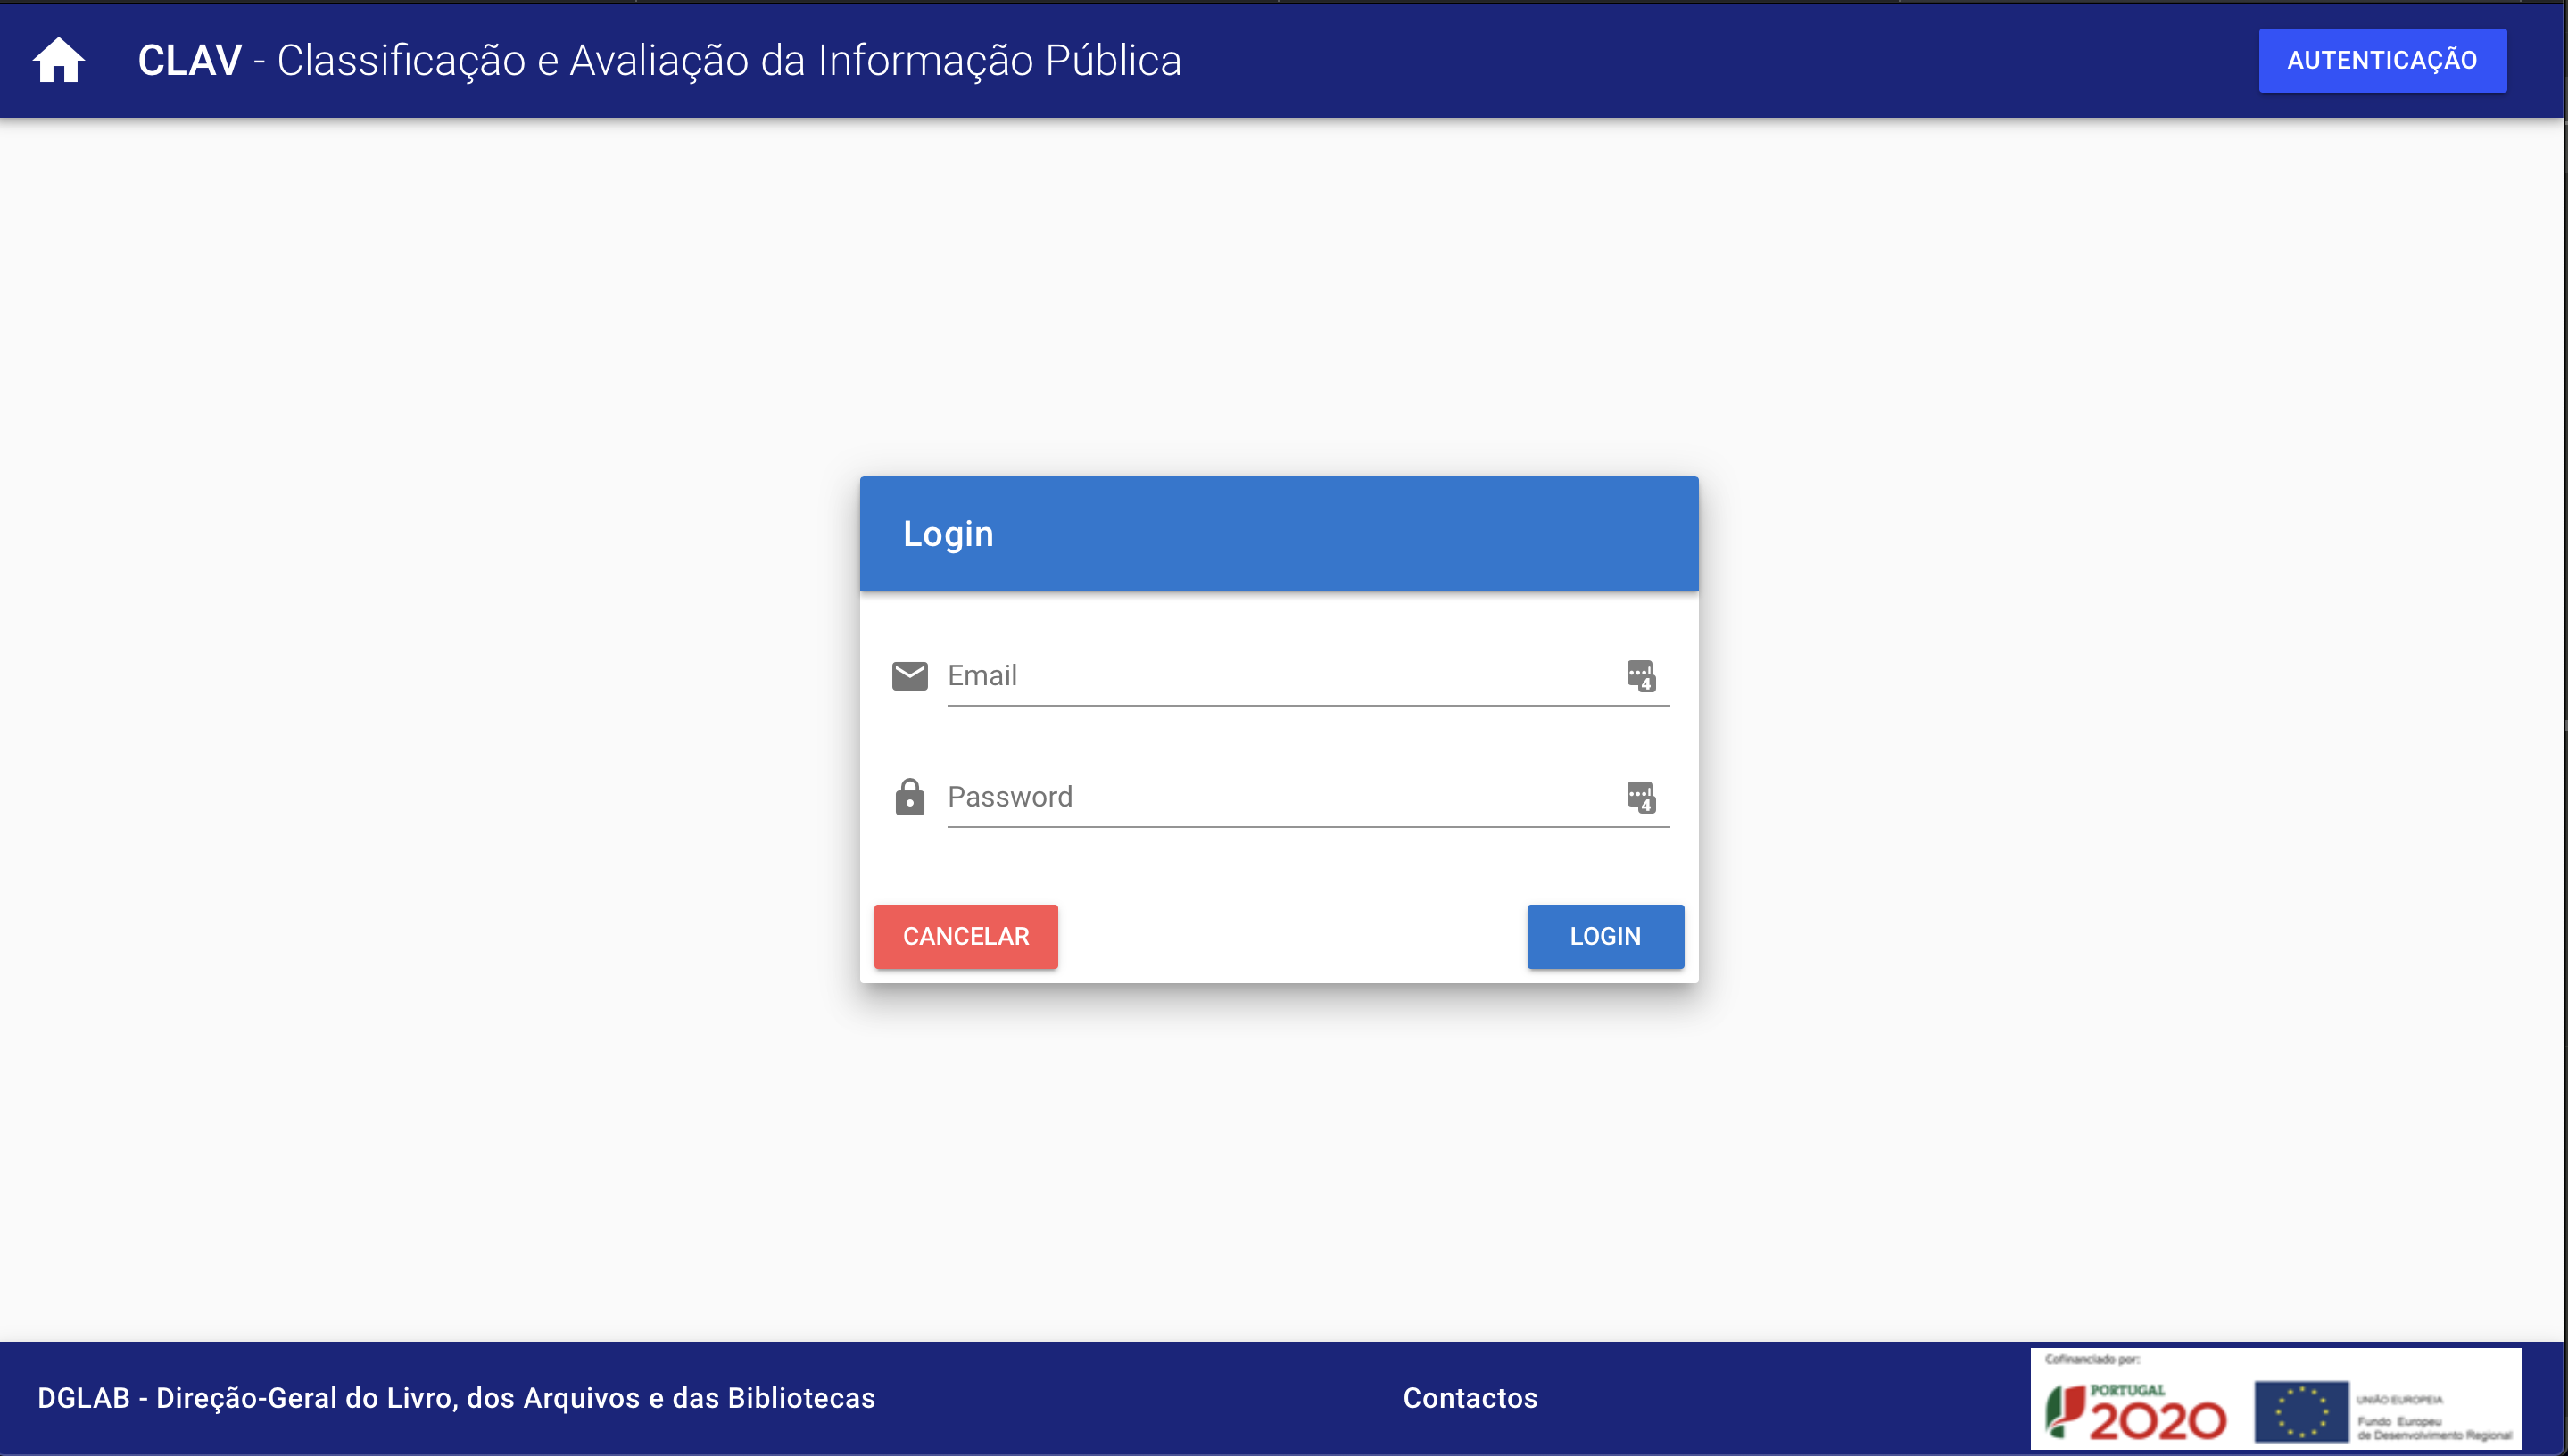
\includegraphics[width=0.95\textwidth]{img/clav/authlocal/login.png}
    \caption{Página de login através de username e password na plataforma \gls{clav}.}
    \label{fig:paginaLoginLocal}
\end{figure}

Após submeter o pedido de login pode ocorrer um dos seguintes cenários:

\begin{itemize}
    \vspace{-2mm}
    \item \textbf{Sucesso}
    
    Ocorre quando o utilizador fornece uma combinação de email e password correta.
    
    \begin{figure}[h!]
        \centering
        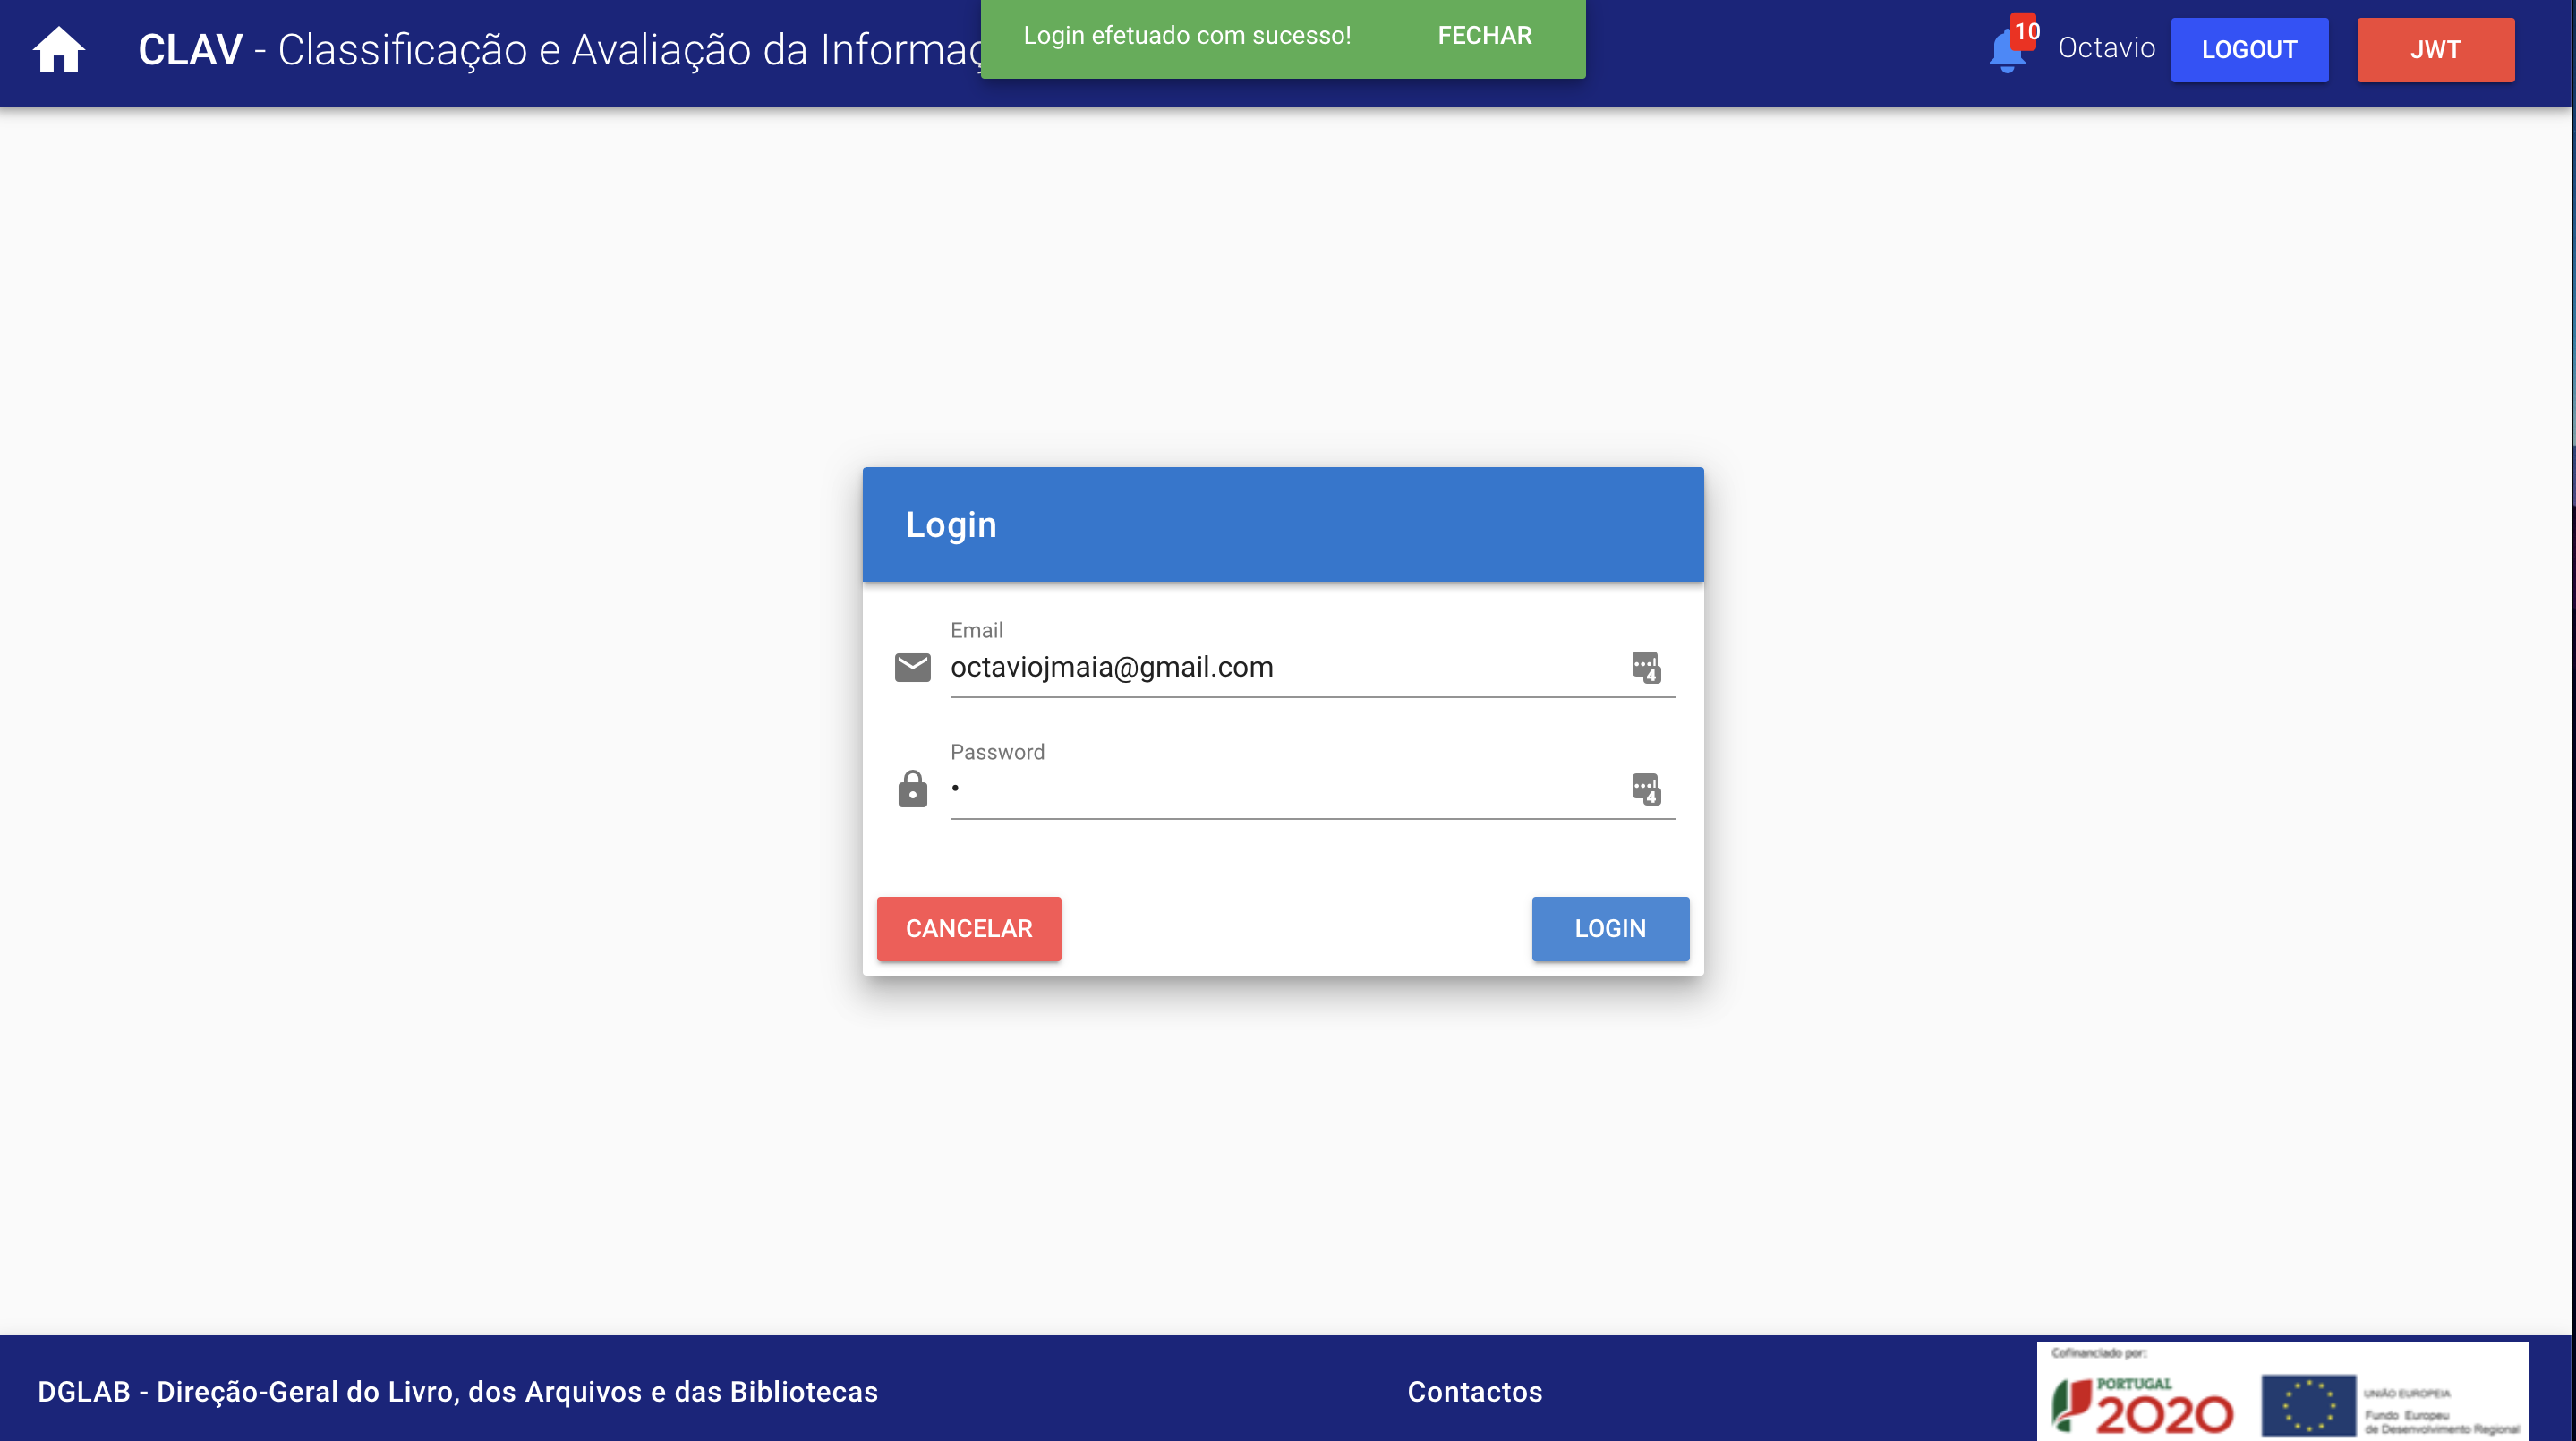
\includegraphics[width=0.95\textwidth]{img/clav/authlocal/sucessoLogin.png}
        \caption{Página quando ocorre um login com sucesso na plataforma \gls{clav}.}
        \label{fig:registoLogin}
    \end{figure}
    
    \item \textbf{Insucesso}
    
    \begin{itemize}
        \item \textbf{Dados insuficientes}
        
        Ocorre quando o utilizador não preencheu todos os campos necessários para o login.
        
        \begin{figure}[h!]
            \centering
            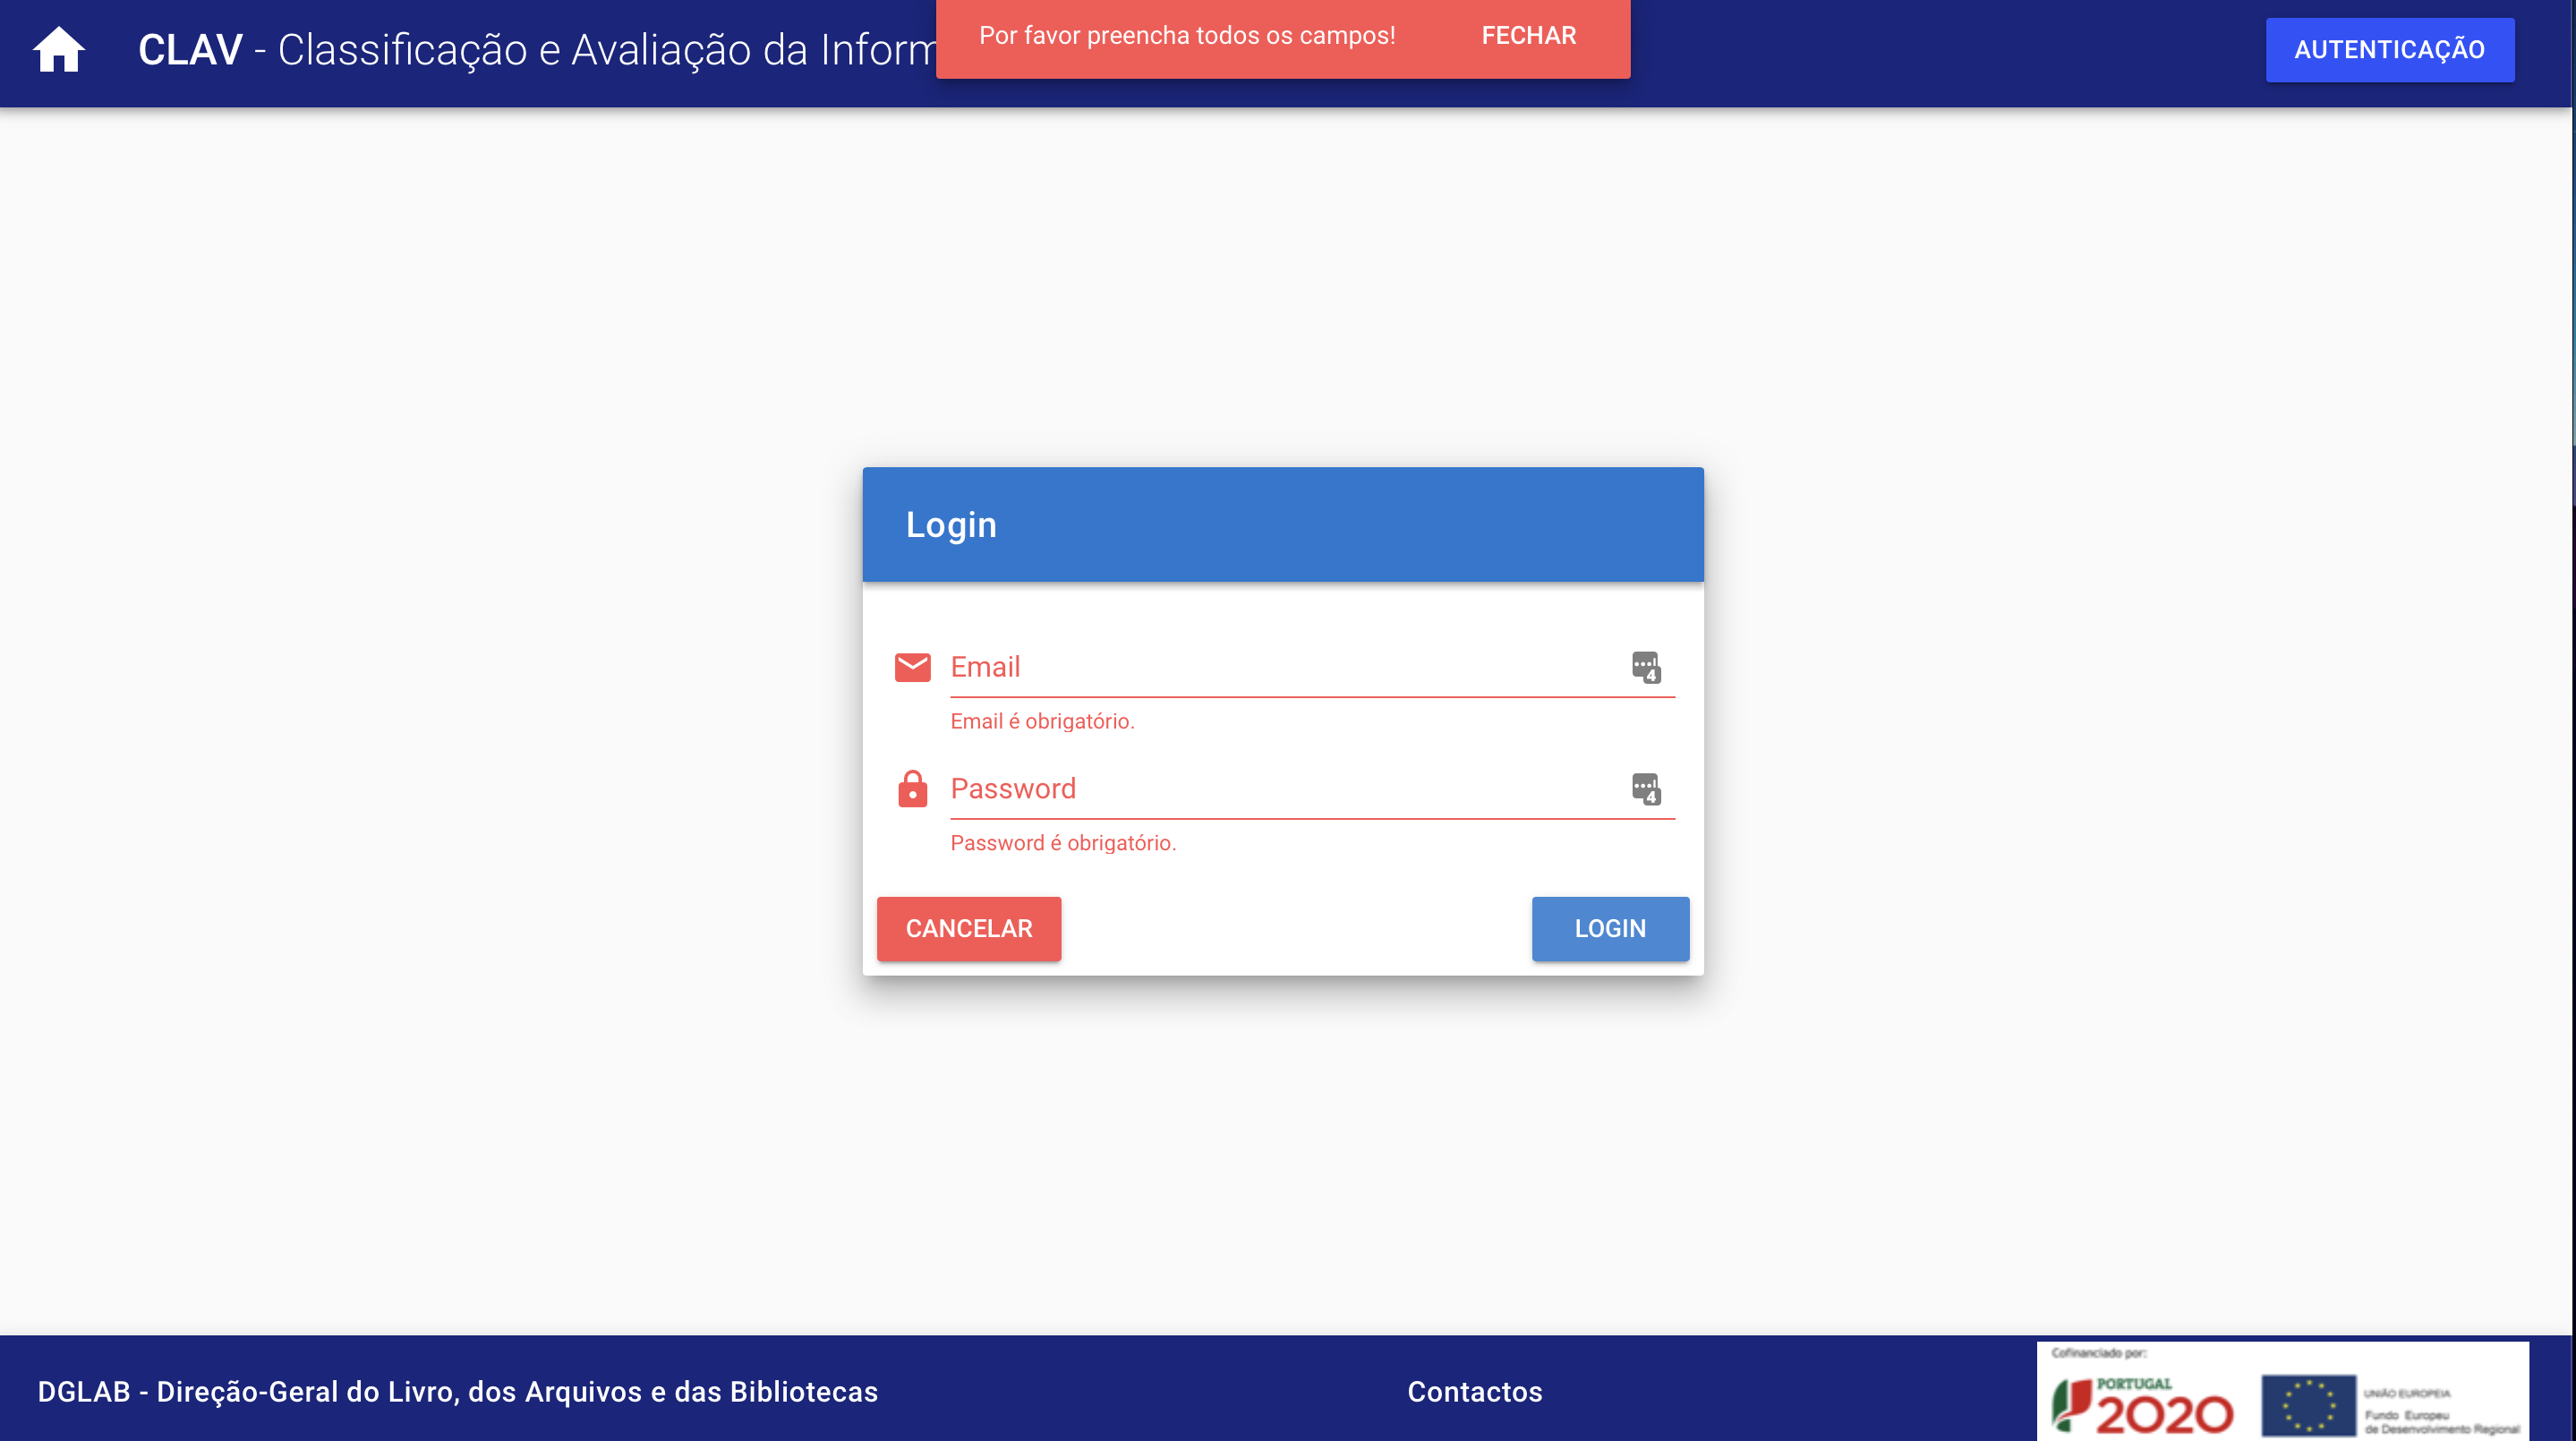
\includegraphics[width=0.95\textwidth]{img/clav/authlocal/erroLogin1.png}
            \caption{Página quando ocorre um erro de login na plataforma \gls{clav}.}
            \label{fig:loginErro1}
        \end{figure}
        
        %\cleardoublepage
        \item \textbf{Dados incorretos}
        
        Ocorre quando o utilizador fornece uma combinação de email e password incorreta.
        
        \begin{figure}[h!]
            \centering
            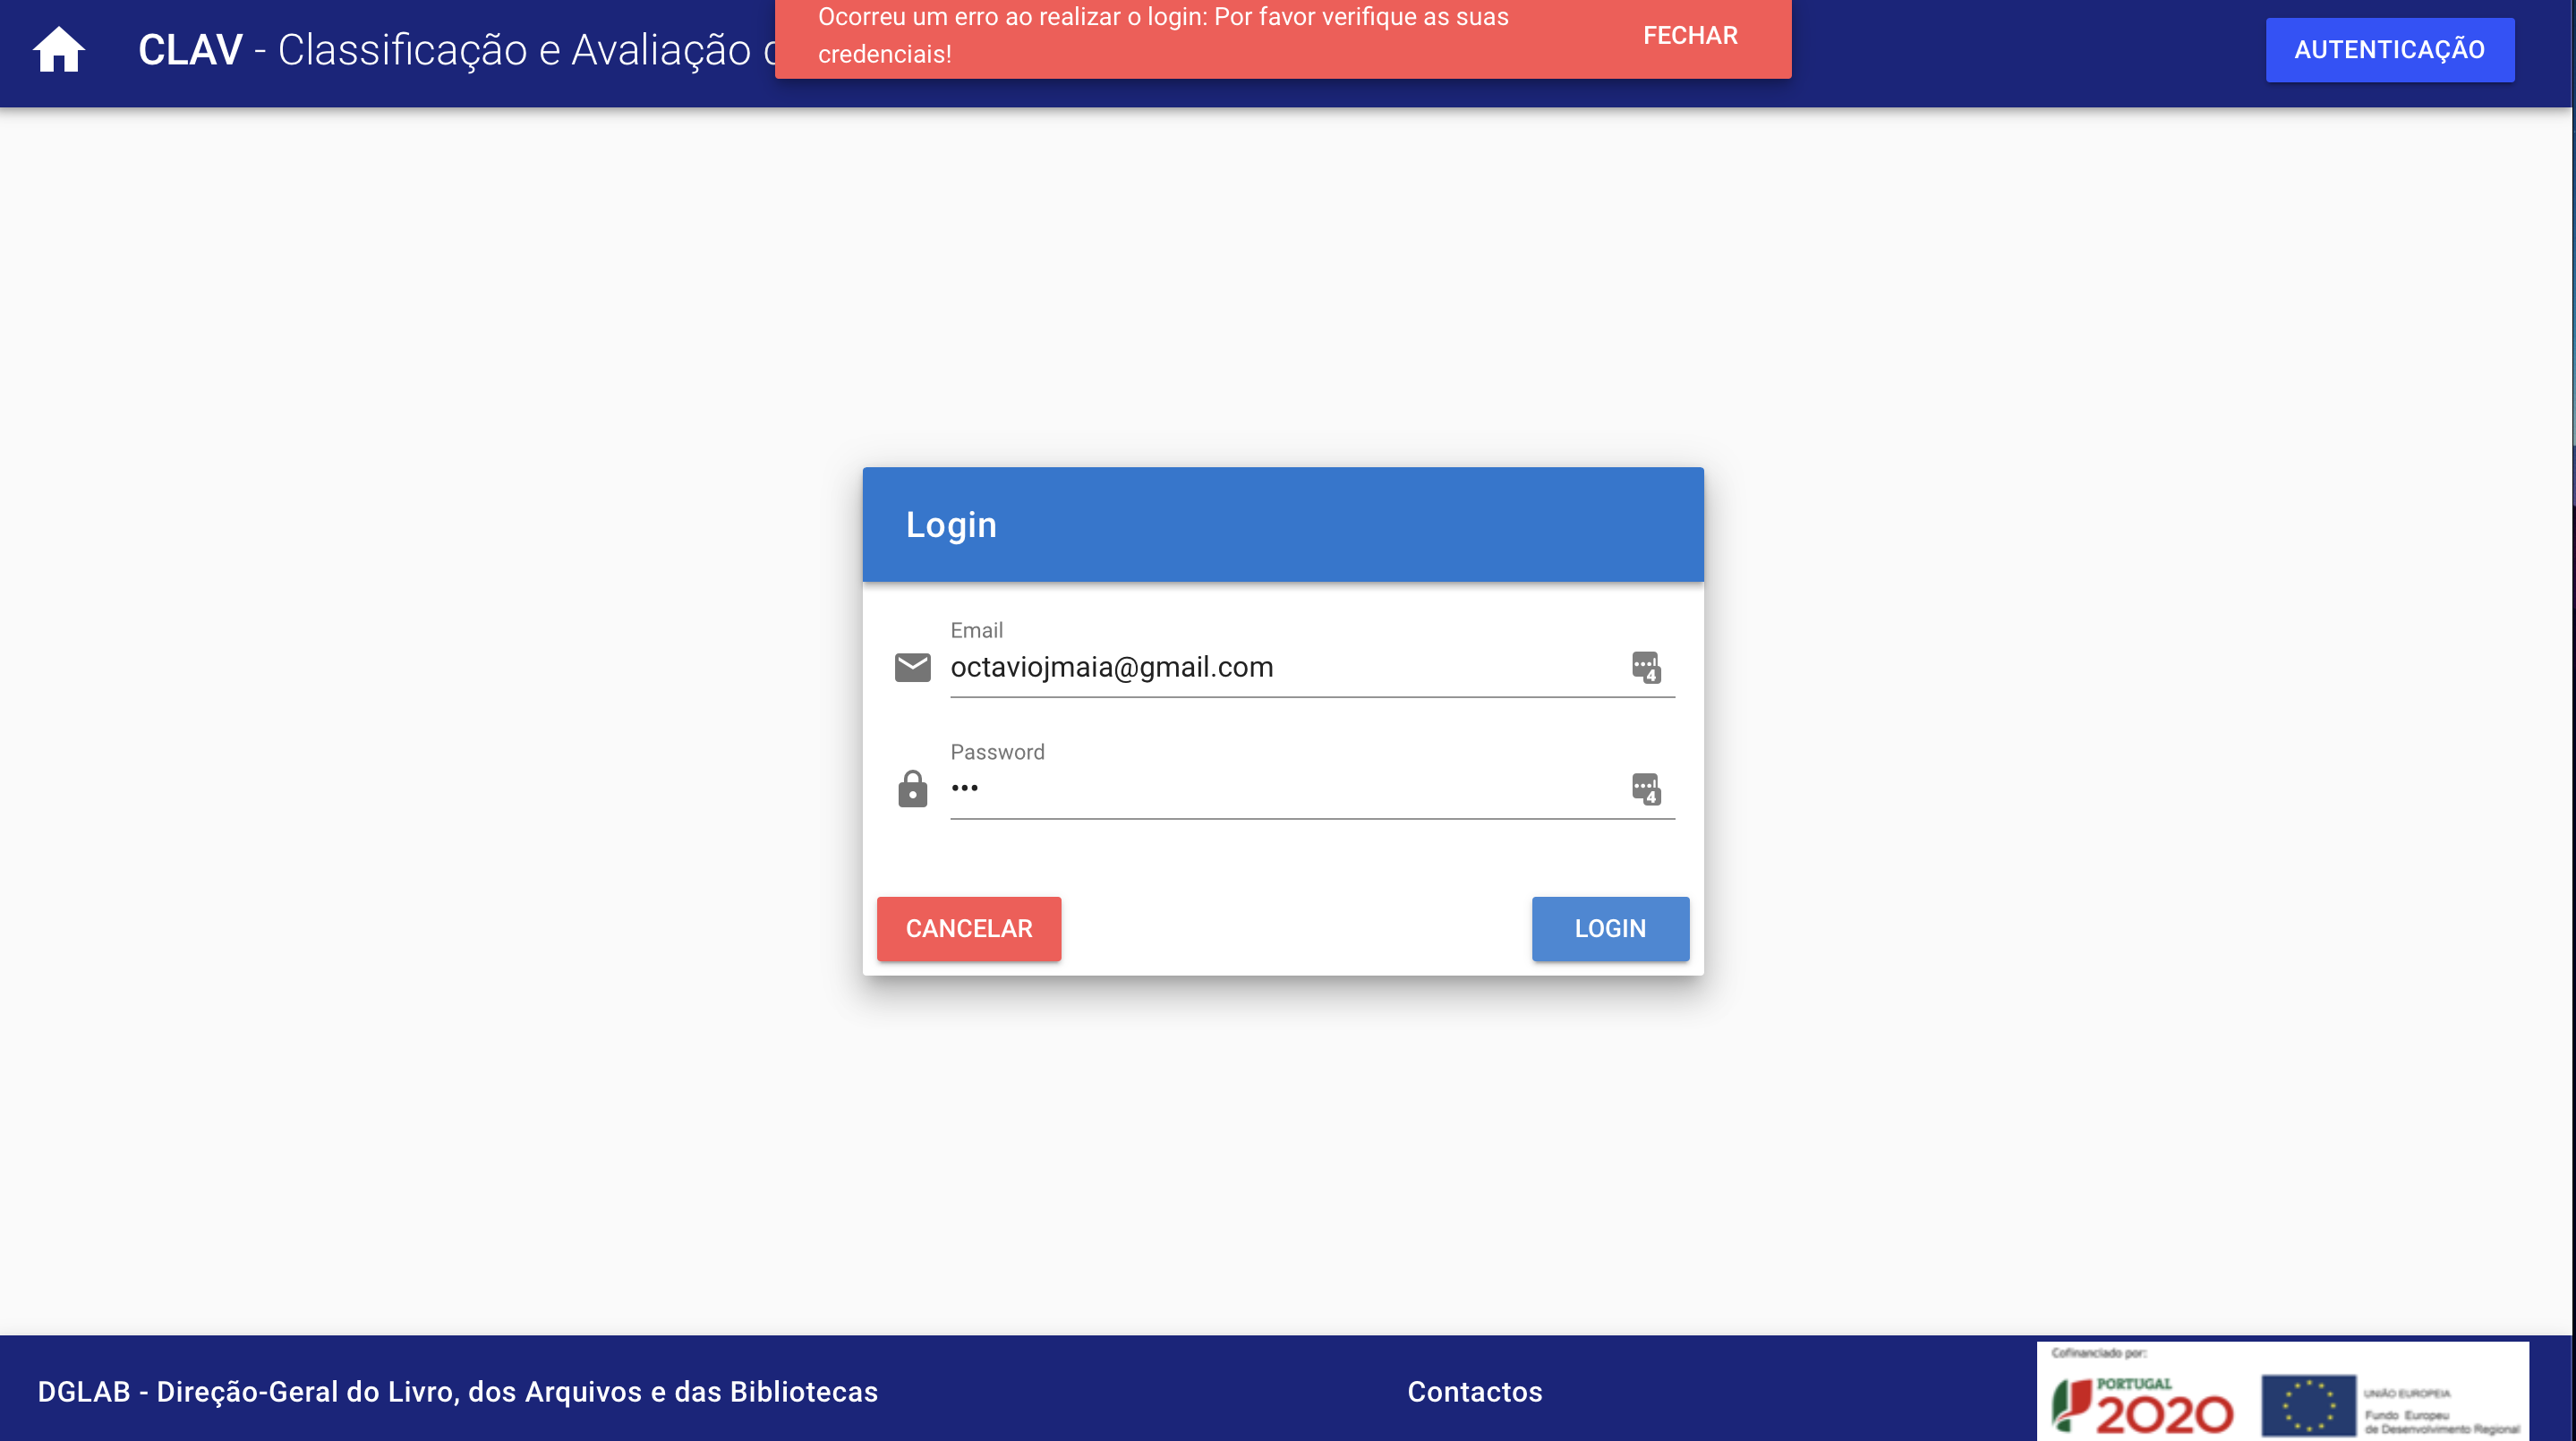
\includegraphics[width=0.95\textwidth]{img/clav/authlocal/erroLogin2.png}
            \caption{Página quando ocorre um erro de login na plataforma \gls{clav}.}
            \label{fig:loginErro2}
        \end{figure}
    \end{itemize}
\end{itemize}

O comportamento da função de login pode ser explicado pelo diagrama de sequência da figura \ref{fig:diagramaLogin}.

\begin{figure}[h!]
    \centering
    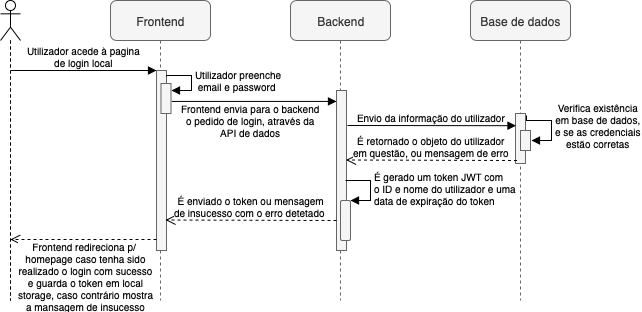
\includegraphics[width=\textwidth]{img/diagramas/sequencia/DiagramasSequencia-Login.png}
    \caption{Diagrama de sequência correspondente ao processo de login local na plataforma \gls{clav}.}
    \label{fig:diagramaLogin}
\end{figure}

\cleardoublepage
\subsubsection{Recuperação de credenciais}

Caso o utilizador se esqueça das suas credenciais, existe uma página de recuperação, indicada na figura \ref{fig:pagRecuperacao}. Nesta página apenas é necessária a inserção do email utilizado para registo.

\vspace{-3mm}
\begin{figure}[h!]
    \centering
    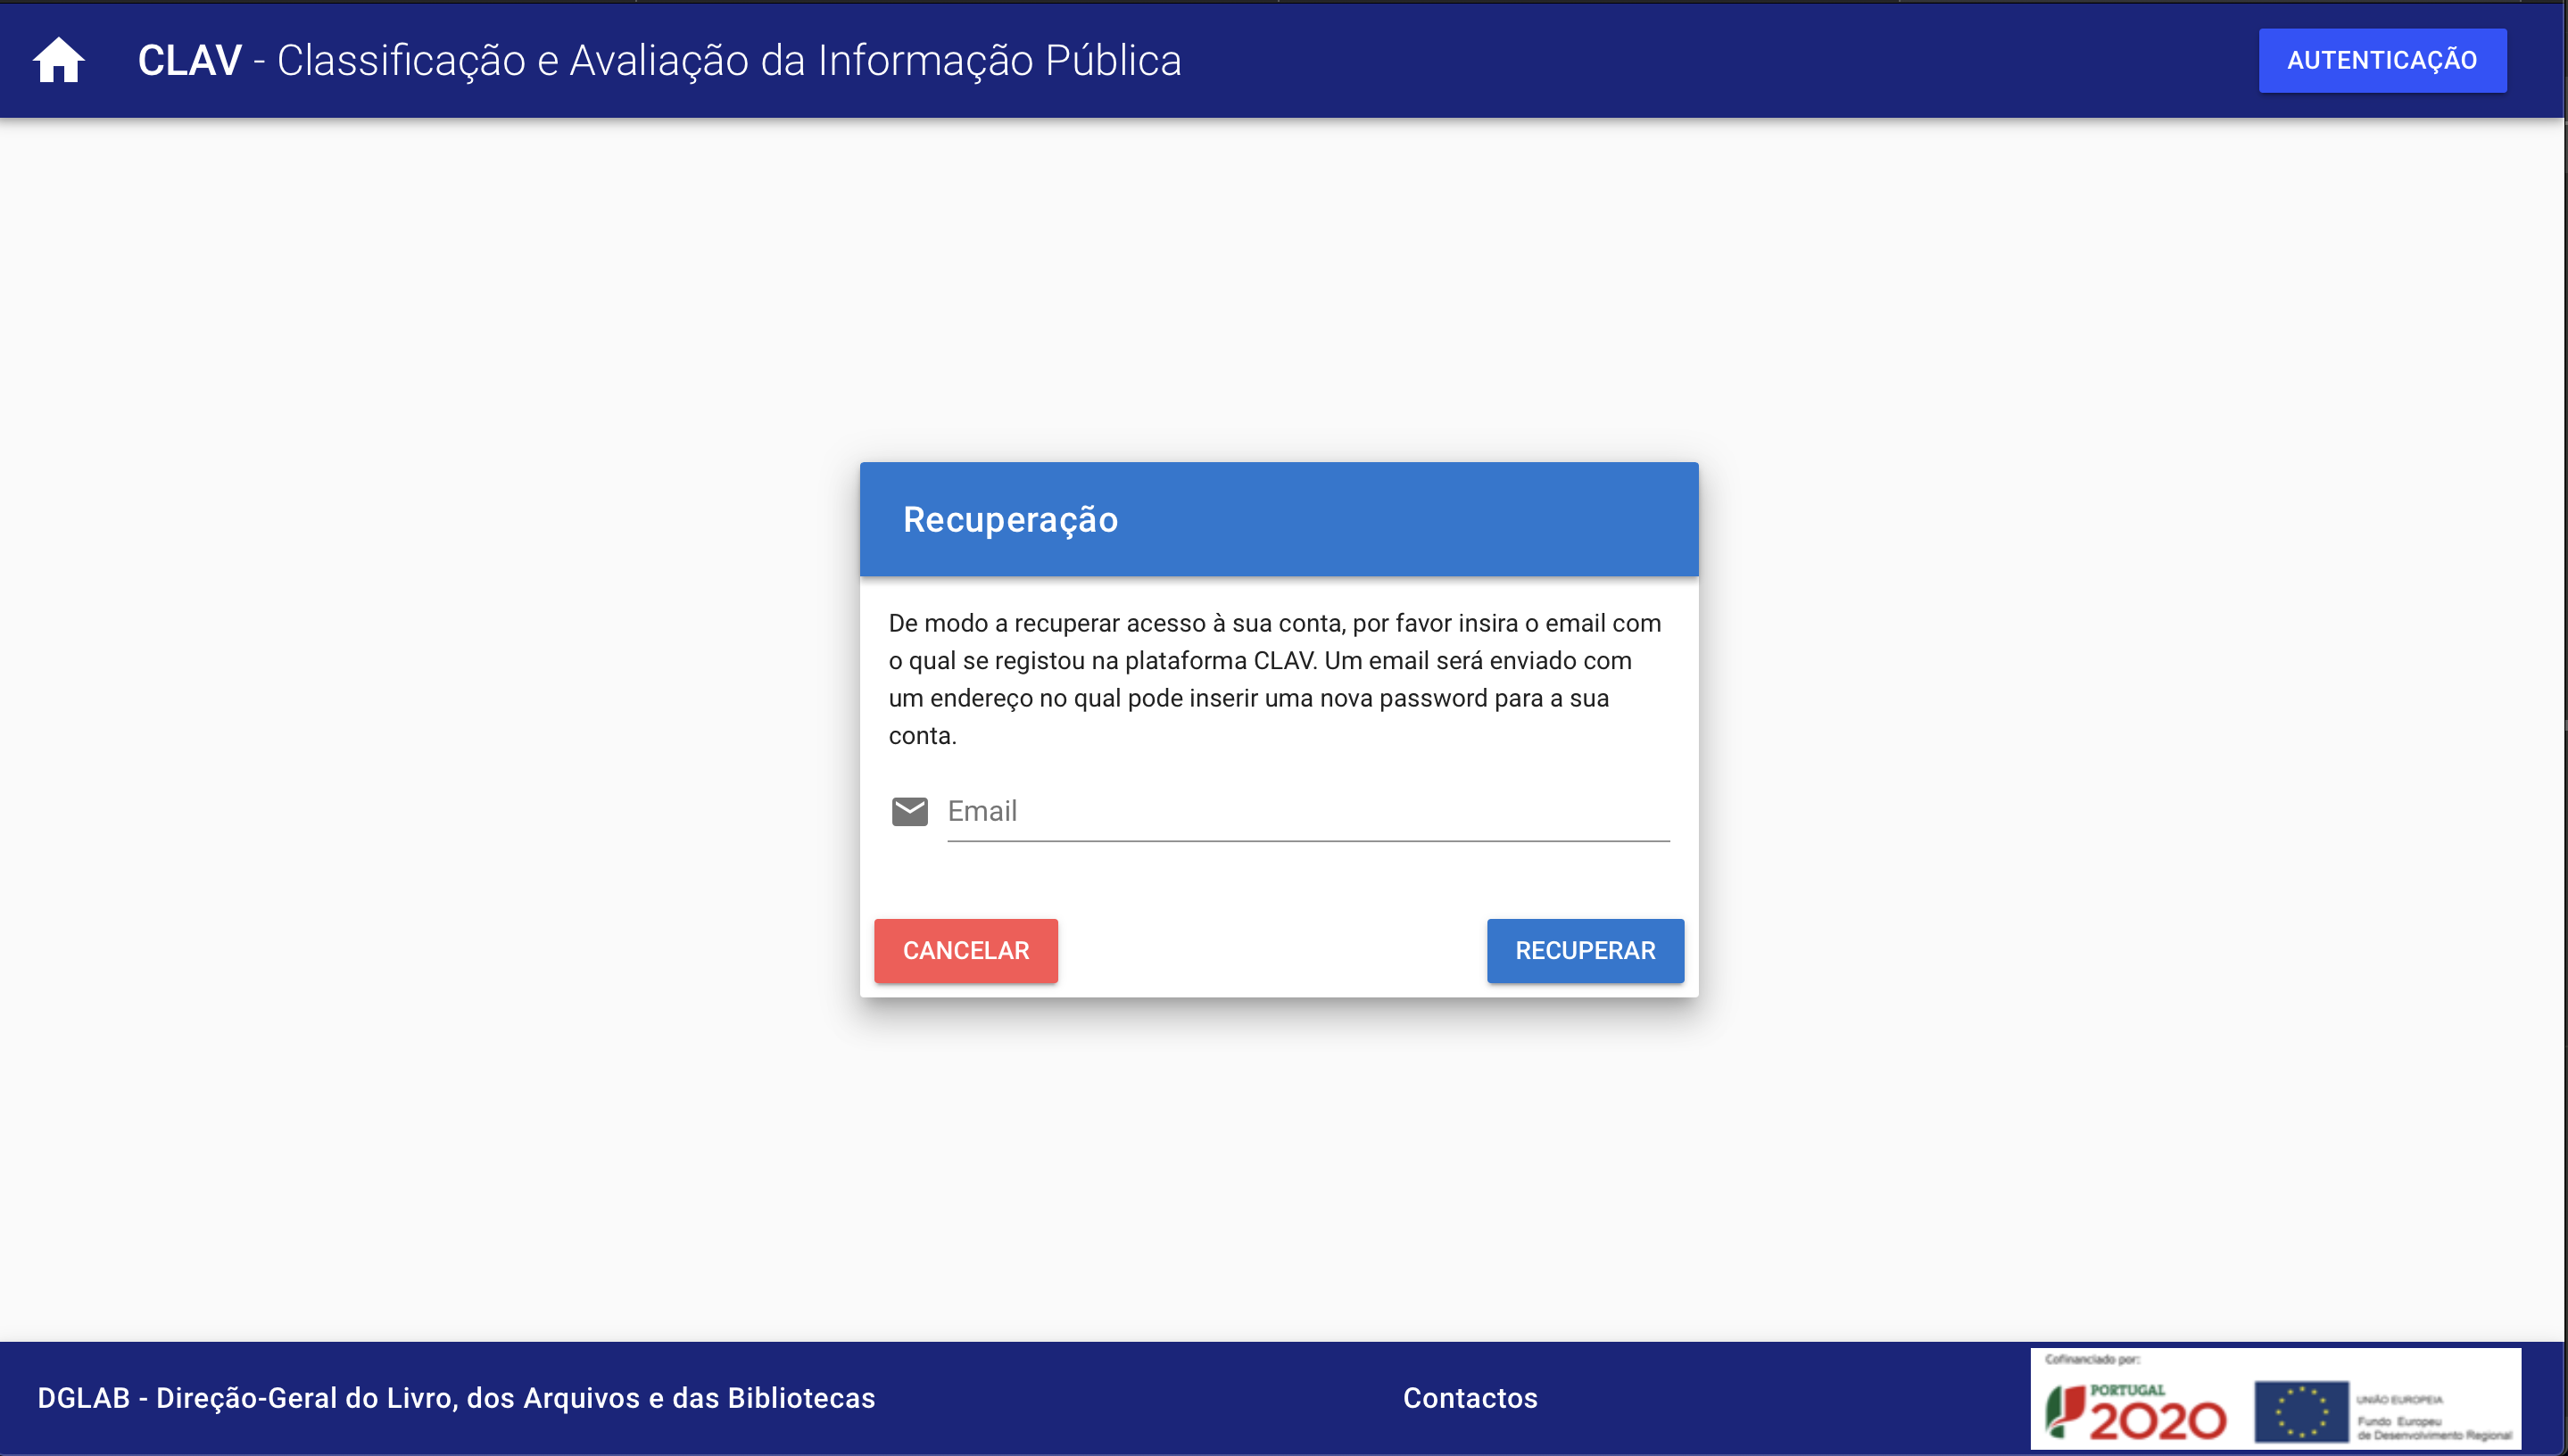
\includegraphics[width=0.9\textwidth]{img/clav/recuperacao/recuperacao.png}
    \caption{Página de recuperação de credenciais na plataforma \gls{clav}.}
    \label{fig:pagRecuperacao}
\end{figure}

\vspace{-3mm}
Após inserção do email e subsequente pedido de recuperação de credenciais, pode ocorrer um dos seguintes cenários:

\vspace{-4mm}
\begin{itemize}
    \item \textbf{Sucesso}
    
    Ocorre quando o utilizador fornece um email presente em base de dados.
    
    \vspace{-4mm}
    \begin{figure}[H]
        \centering
        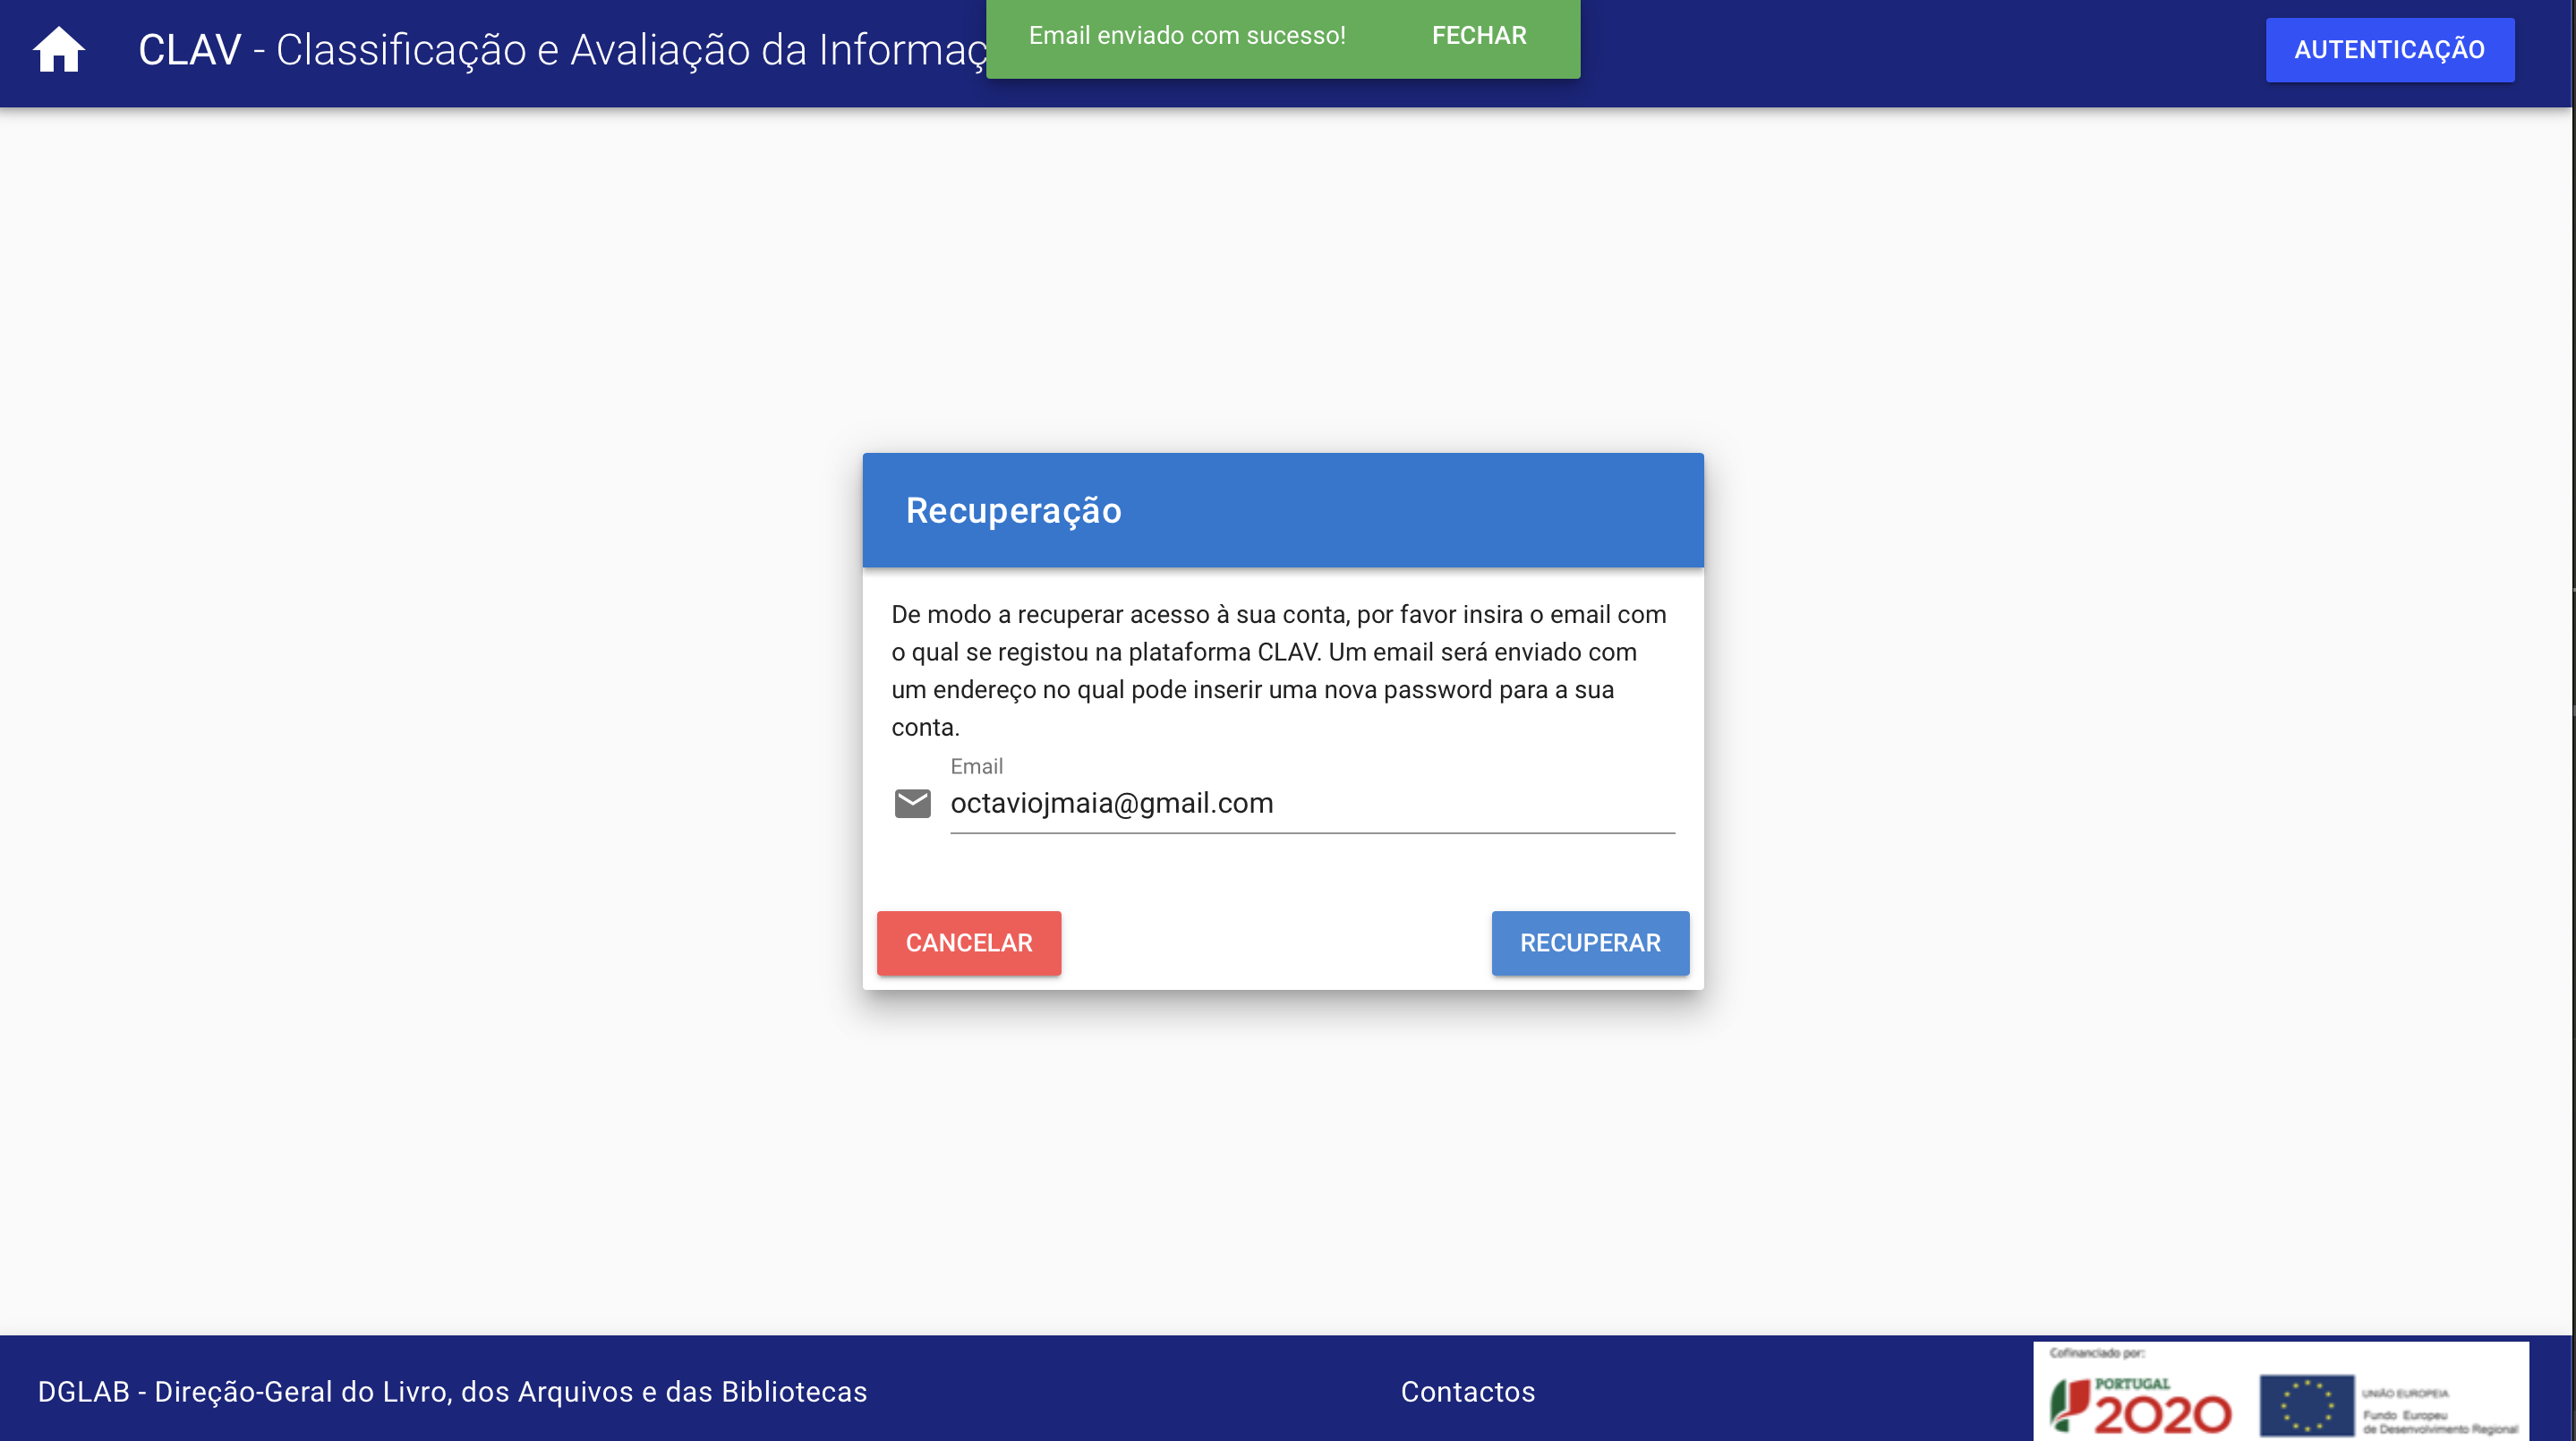
\includegraphics[width=0.9\textwidth]{img/clav/recuperacao/recuperacaoEnviado.png}
        \caption{Mensagem de aviso do envio de email de recuperação.}
        \label{fig:envioEmailRecuperacao}
    \end{figure}
    
    De seguida, é enviado um email para esse destinatário, com um link para recuperação da password. Por questões de segurança este link é válido por 30 minutos, sendo que após esse montante de tempo, o mesmo expira.
    
    \begin{figure}[H]
        \centering
        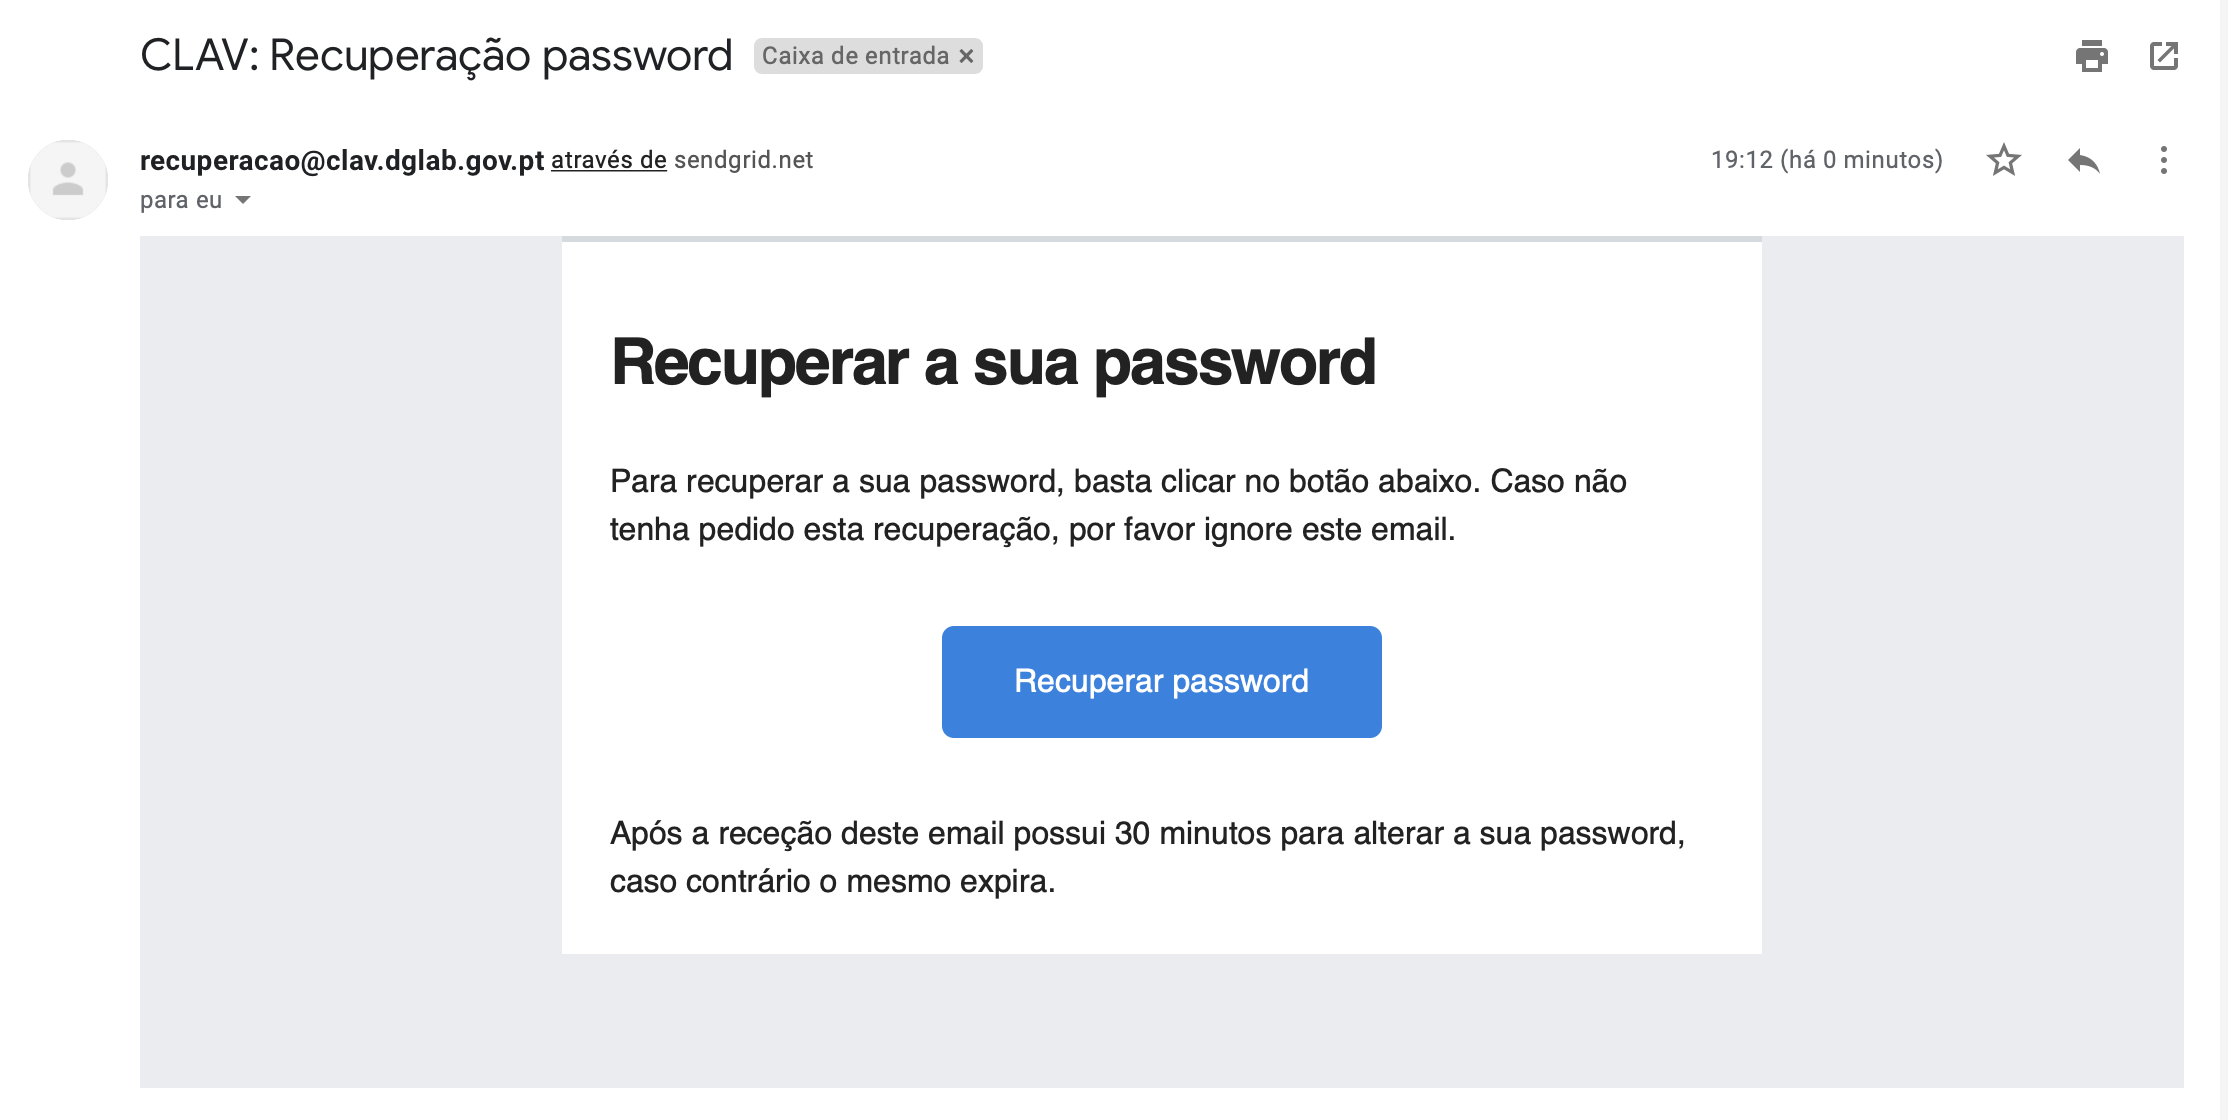
\includegraphics[width=0.9\textwidth]{img/clav/recuperacao/email.png}
        \caption{Email de recuperação enviado pela plataforma \gls{clav}.}
        \label{fig:emailRecuperacao}
    \end{figure}
    
    Após aceder ao link de recuperação, é possível alterar a sua password, exemplificado na figura \ref{fig:pagRecuperacaoSucesso}.
    
    \begin{figure}[H]
        \centering
        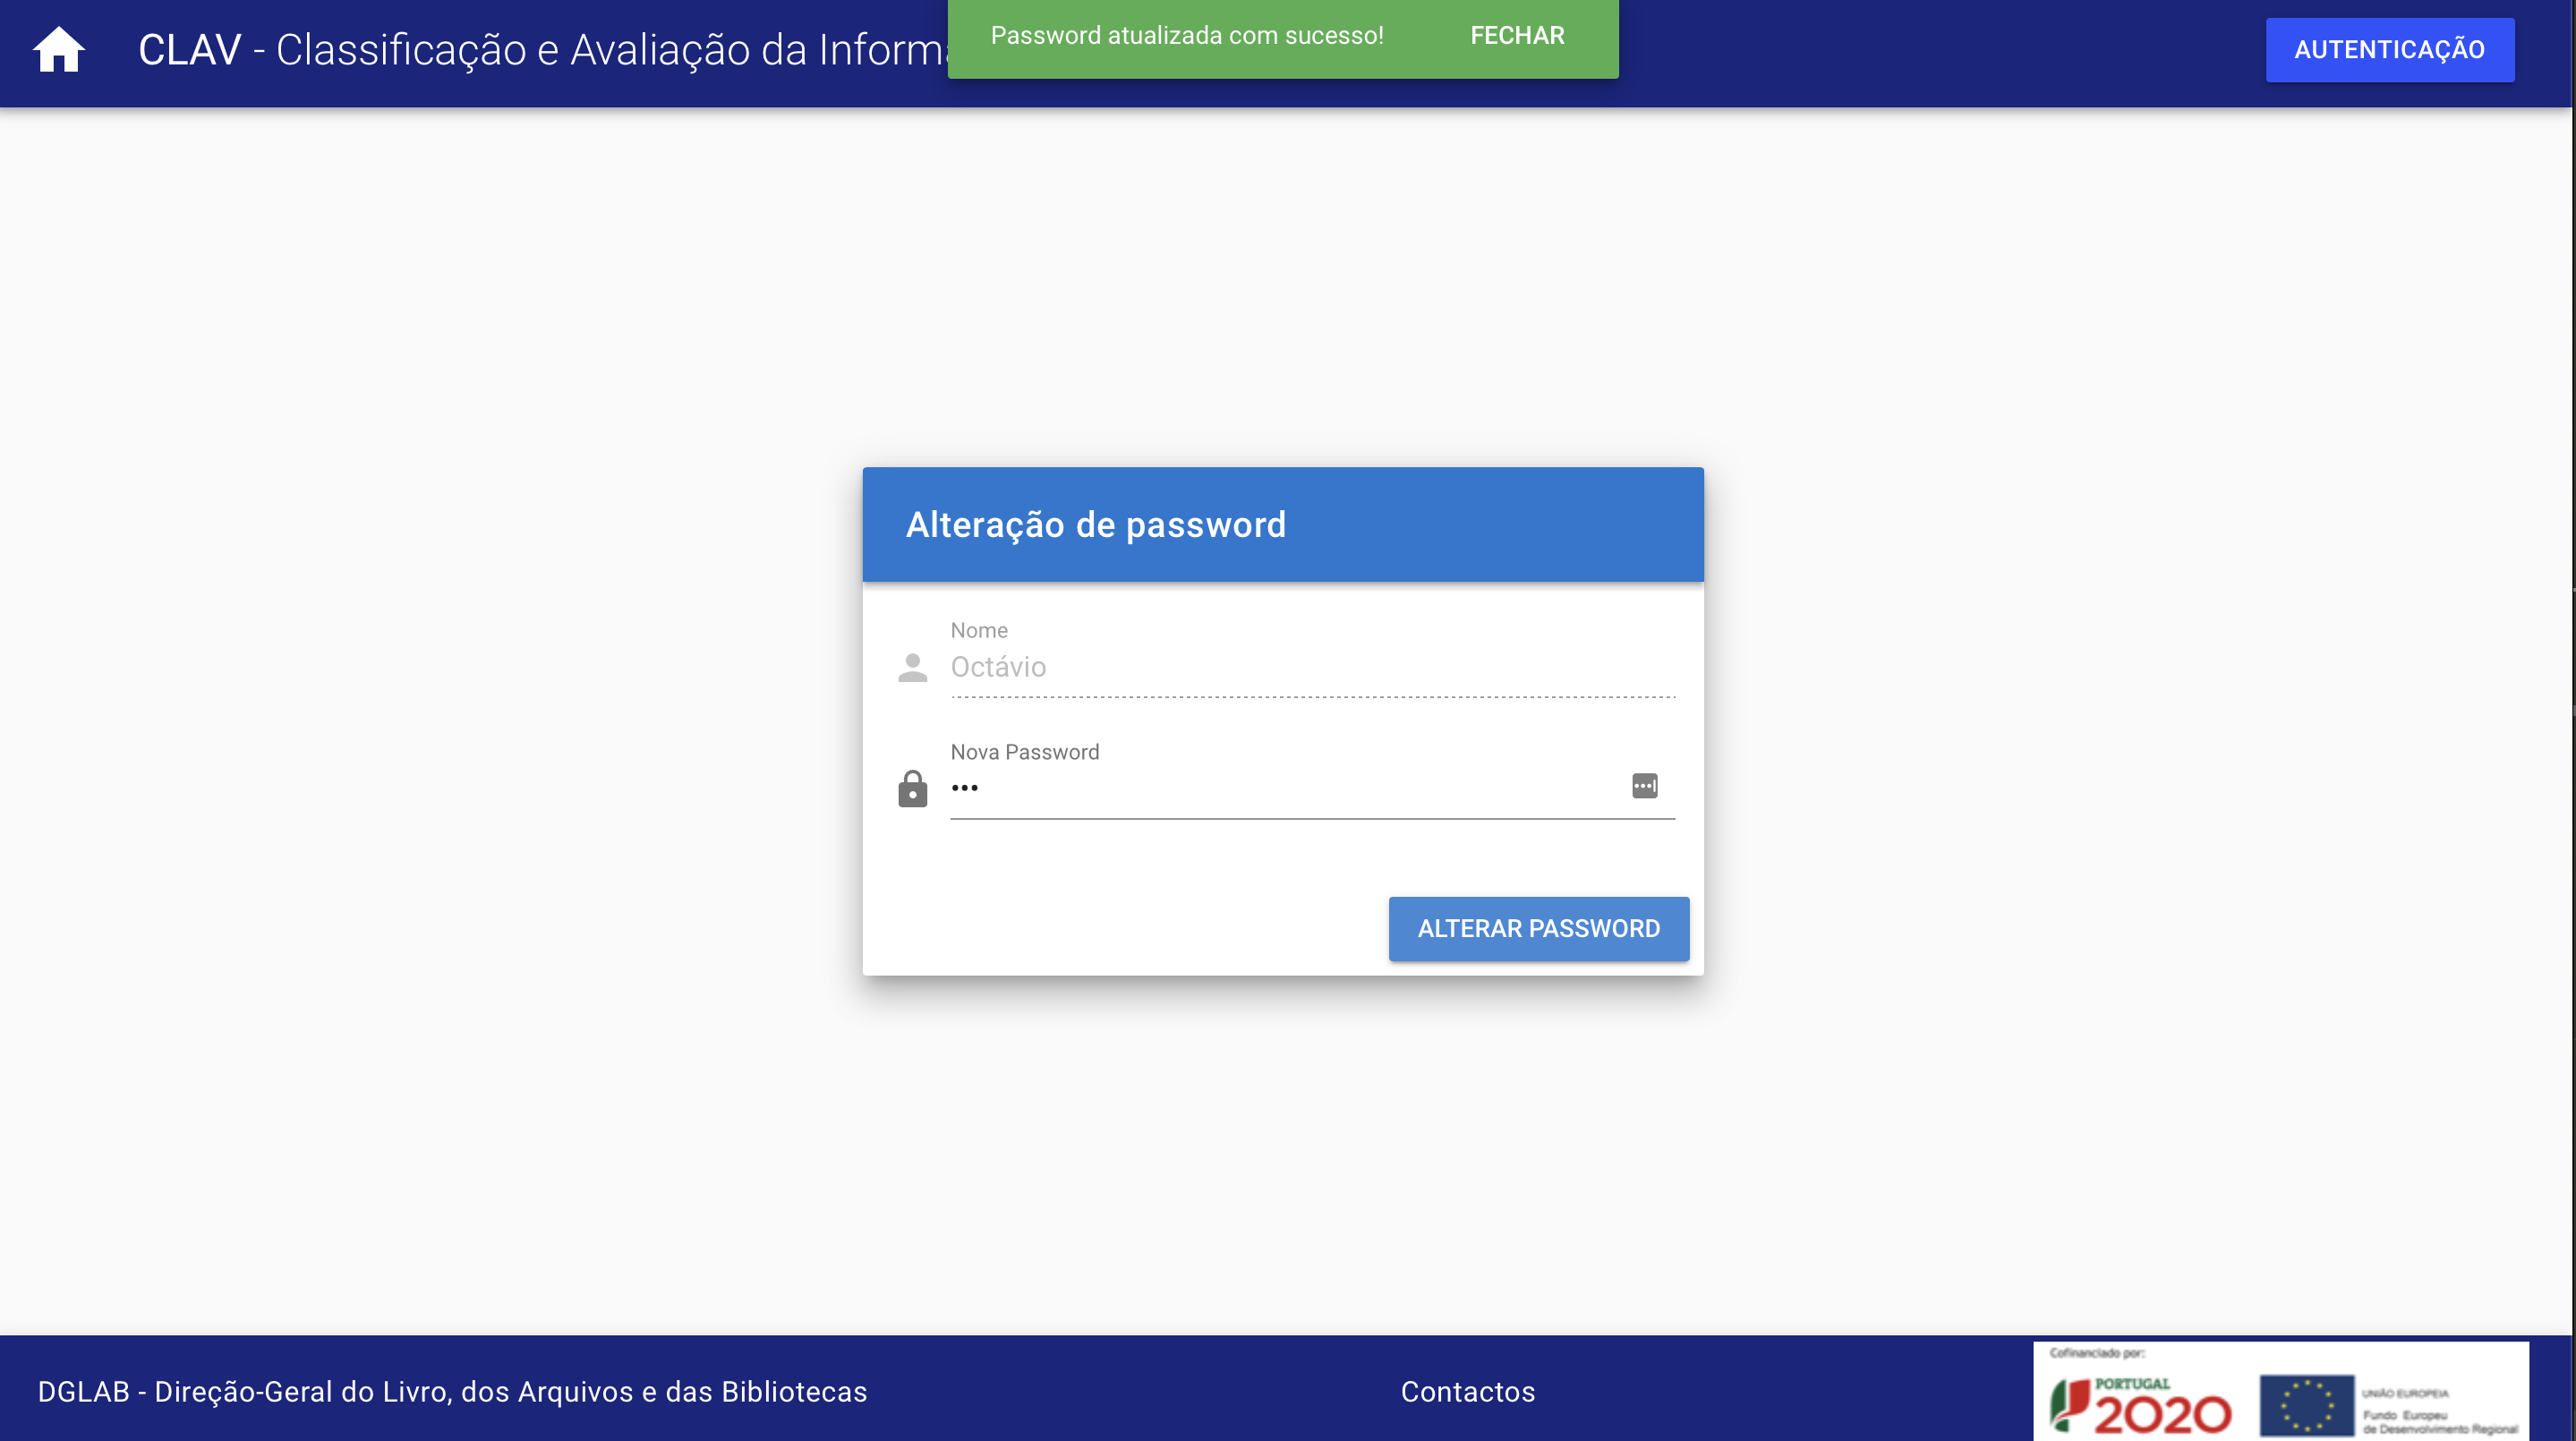
\includegraphics[width=0.9\textwidth]{img/clav/recuperacao/recuperacaoSucesso.png}
        \caption{Mensagem de sucesso após alteração de password na plataforma \gls{clav}.}
        \label{fig:pagRecuperacaoSucesso}
    \end{figure}
    
    \cleardoublepage
    \item \textbf{Insucesso}
    
    \begin{itemize}
        \item \textbf{Dados incorretos}
        
        Ocorre quando o utilizador insere um email que não se encontra presente em base de dados.
        
        \vspace{-2mm}
        \begin{figure}[H]
            \centering
            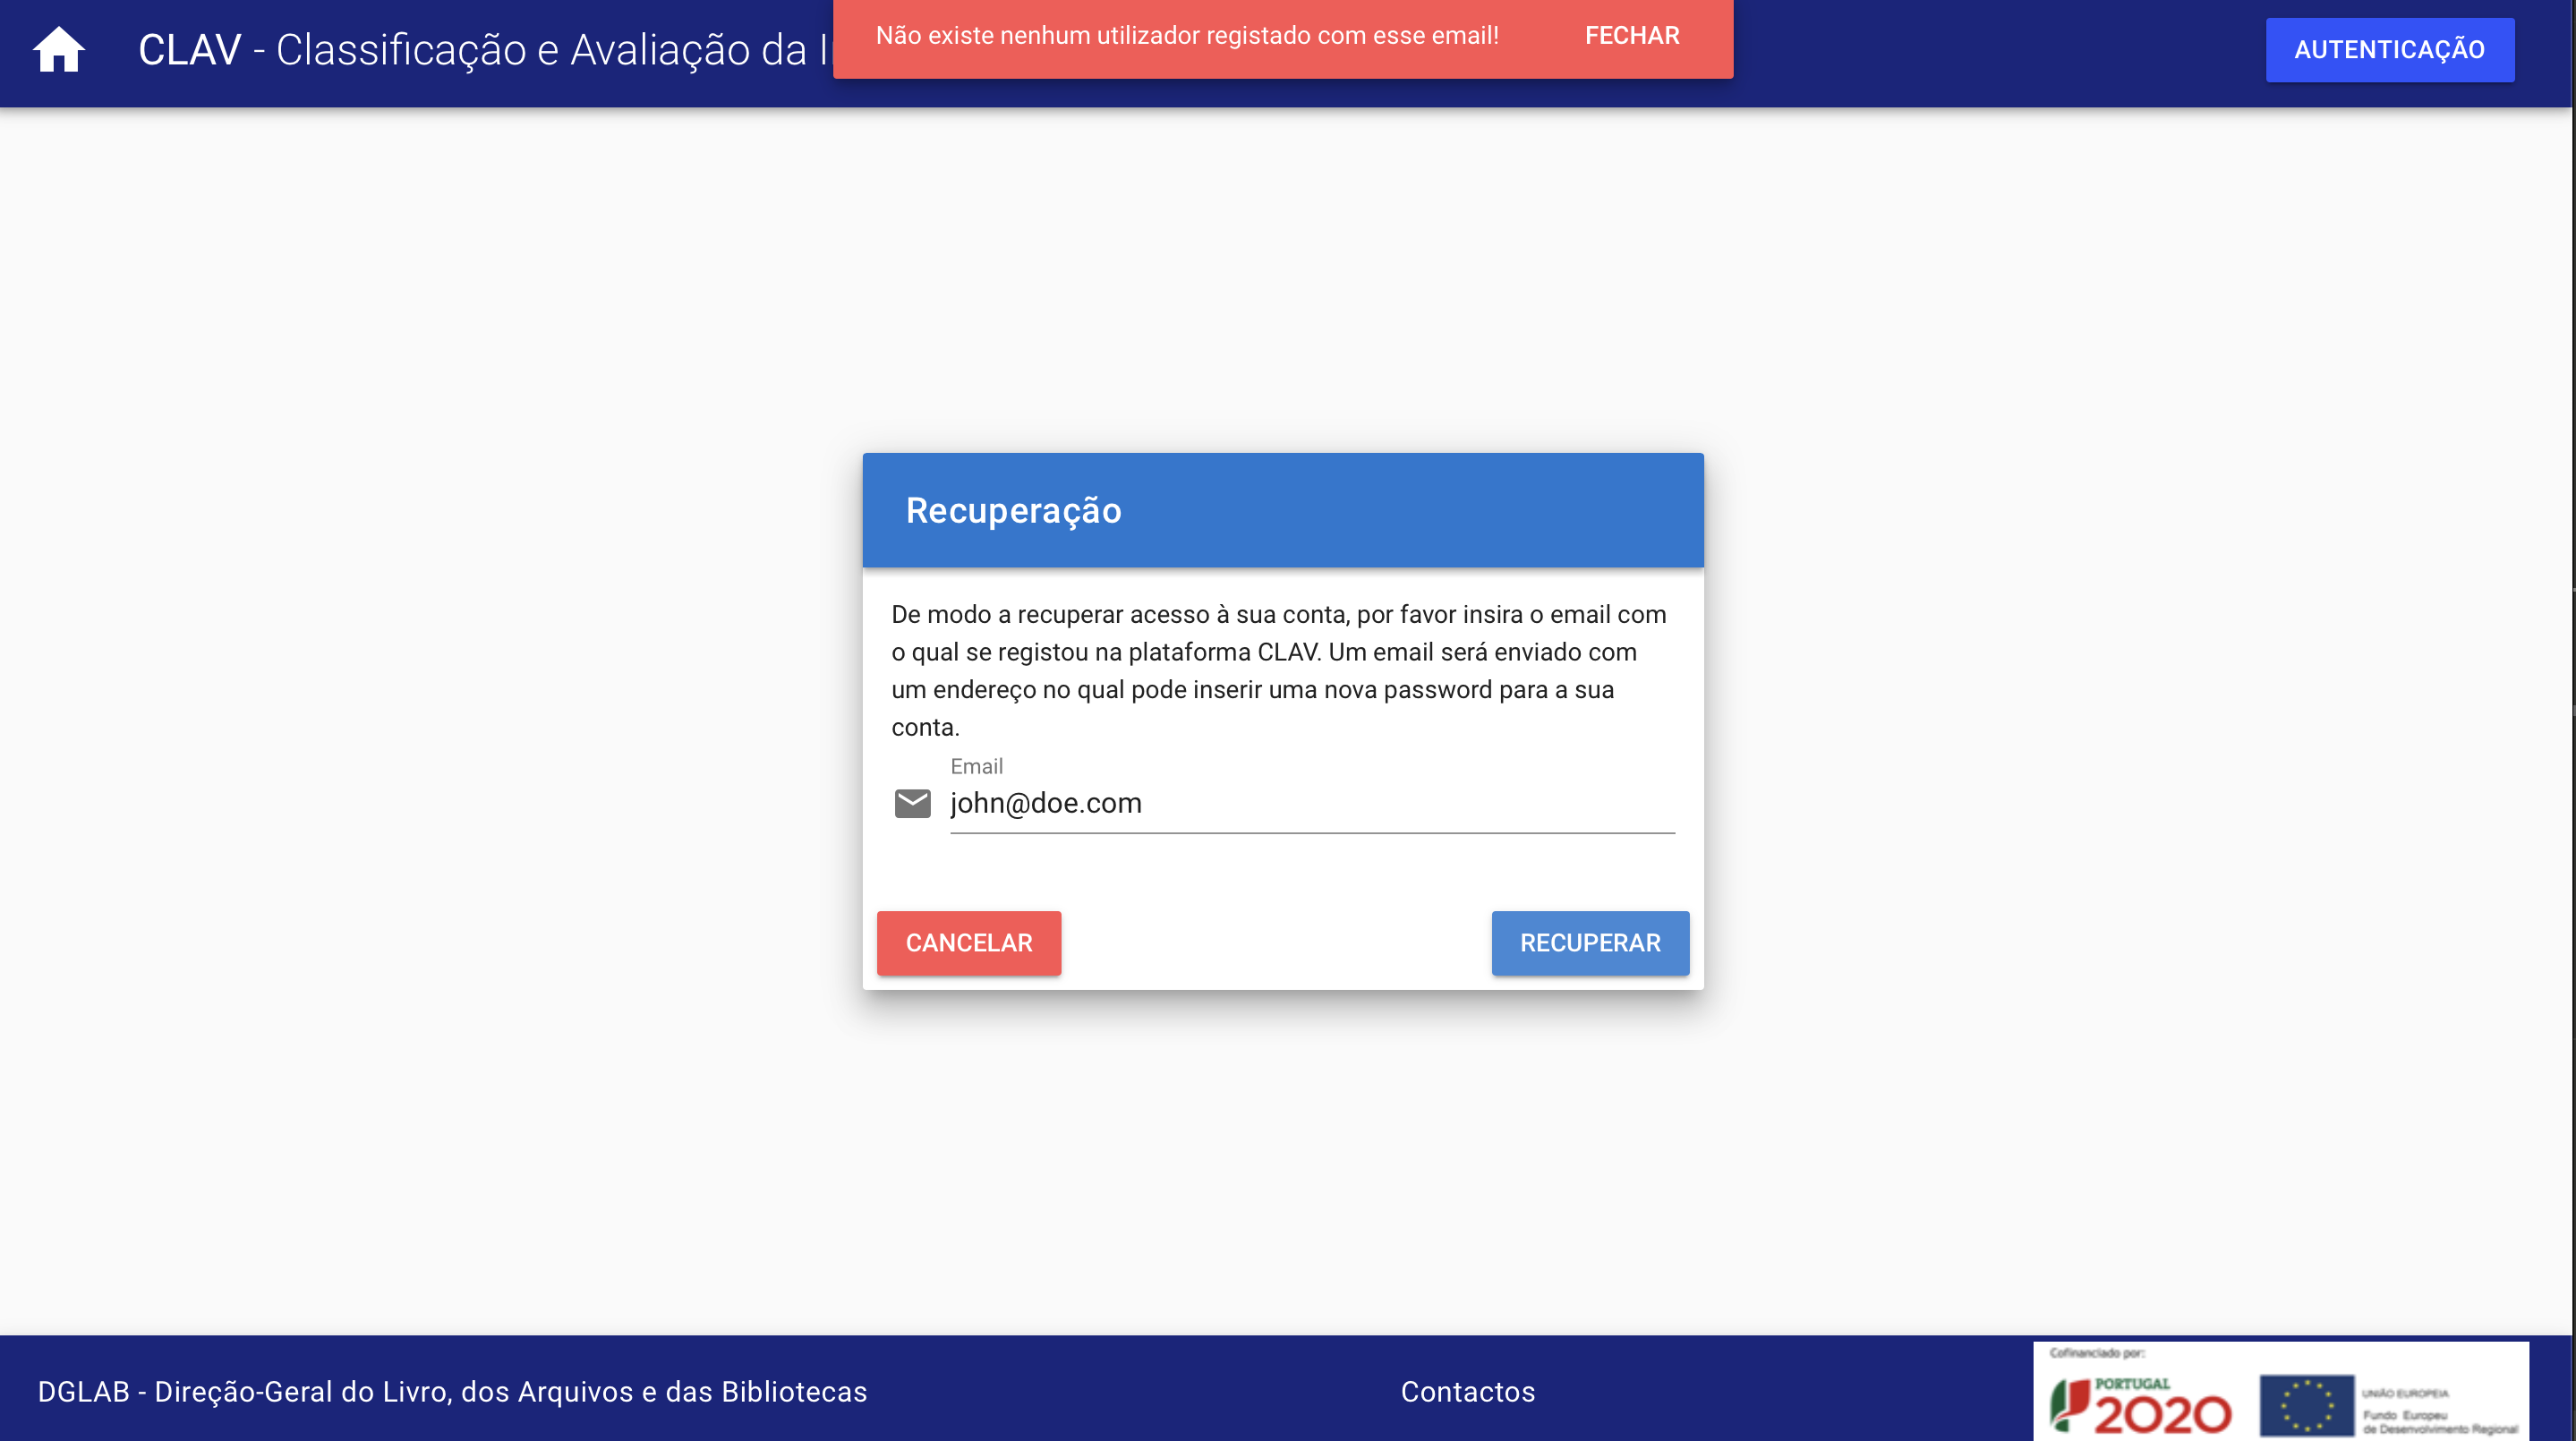
\includegraphics[width=0.9\textwidth]{img/clav/recuperacao/erroEmail.png}
            \caption{Mensagem de erro após inserção de email não existente na plataforma \gls{clav}.}
            \label{fig:pagRecuperacaoErroEmail}
        \end{figure}
        
        \vspace{-5mm}
        \item \textbf{Registo através de Cartão de Cidadão}
        
        Ocorre quando o utilizador insere um email associado a um registo com o Cartão de Cidadão.
    
        \vspace{-2mm}
        \begin{figure}[H]
            \centering
            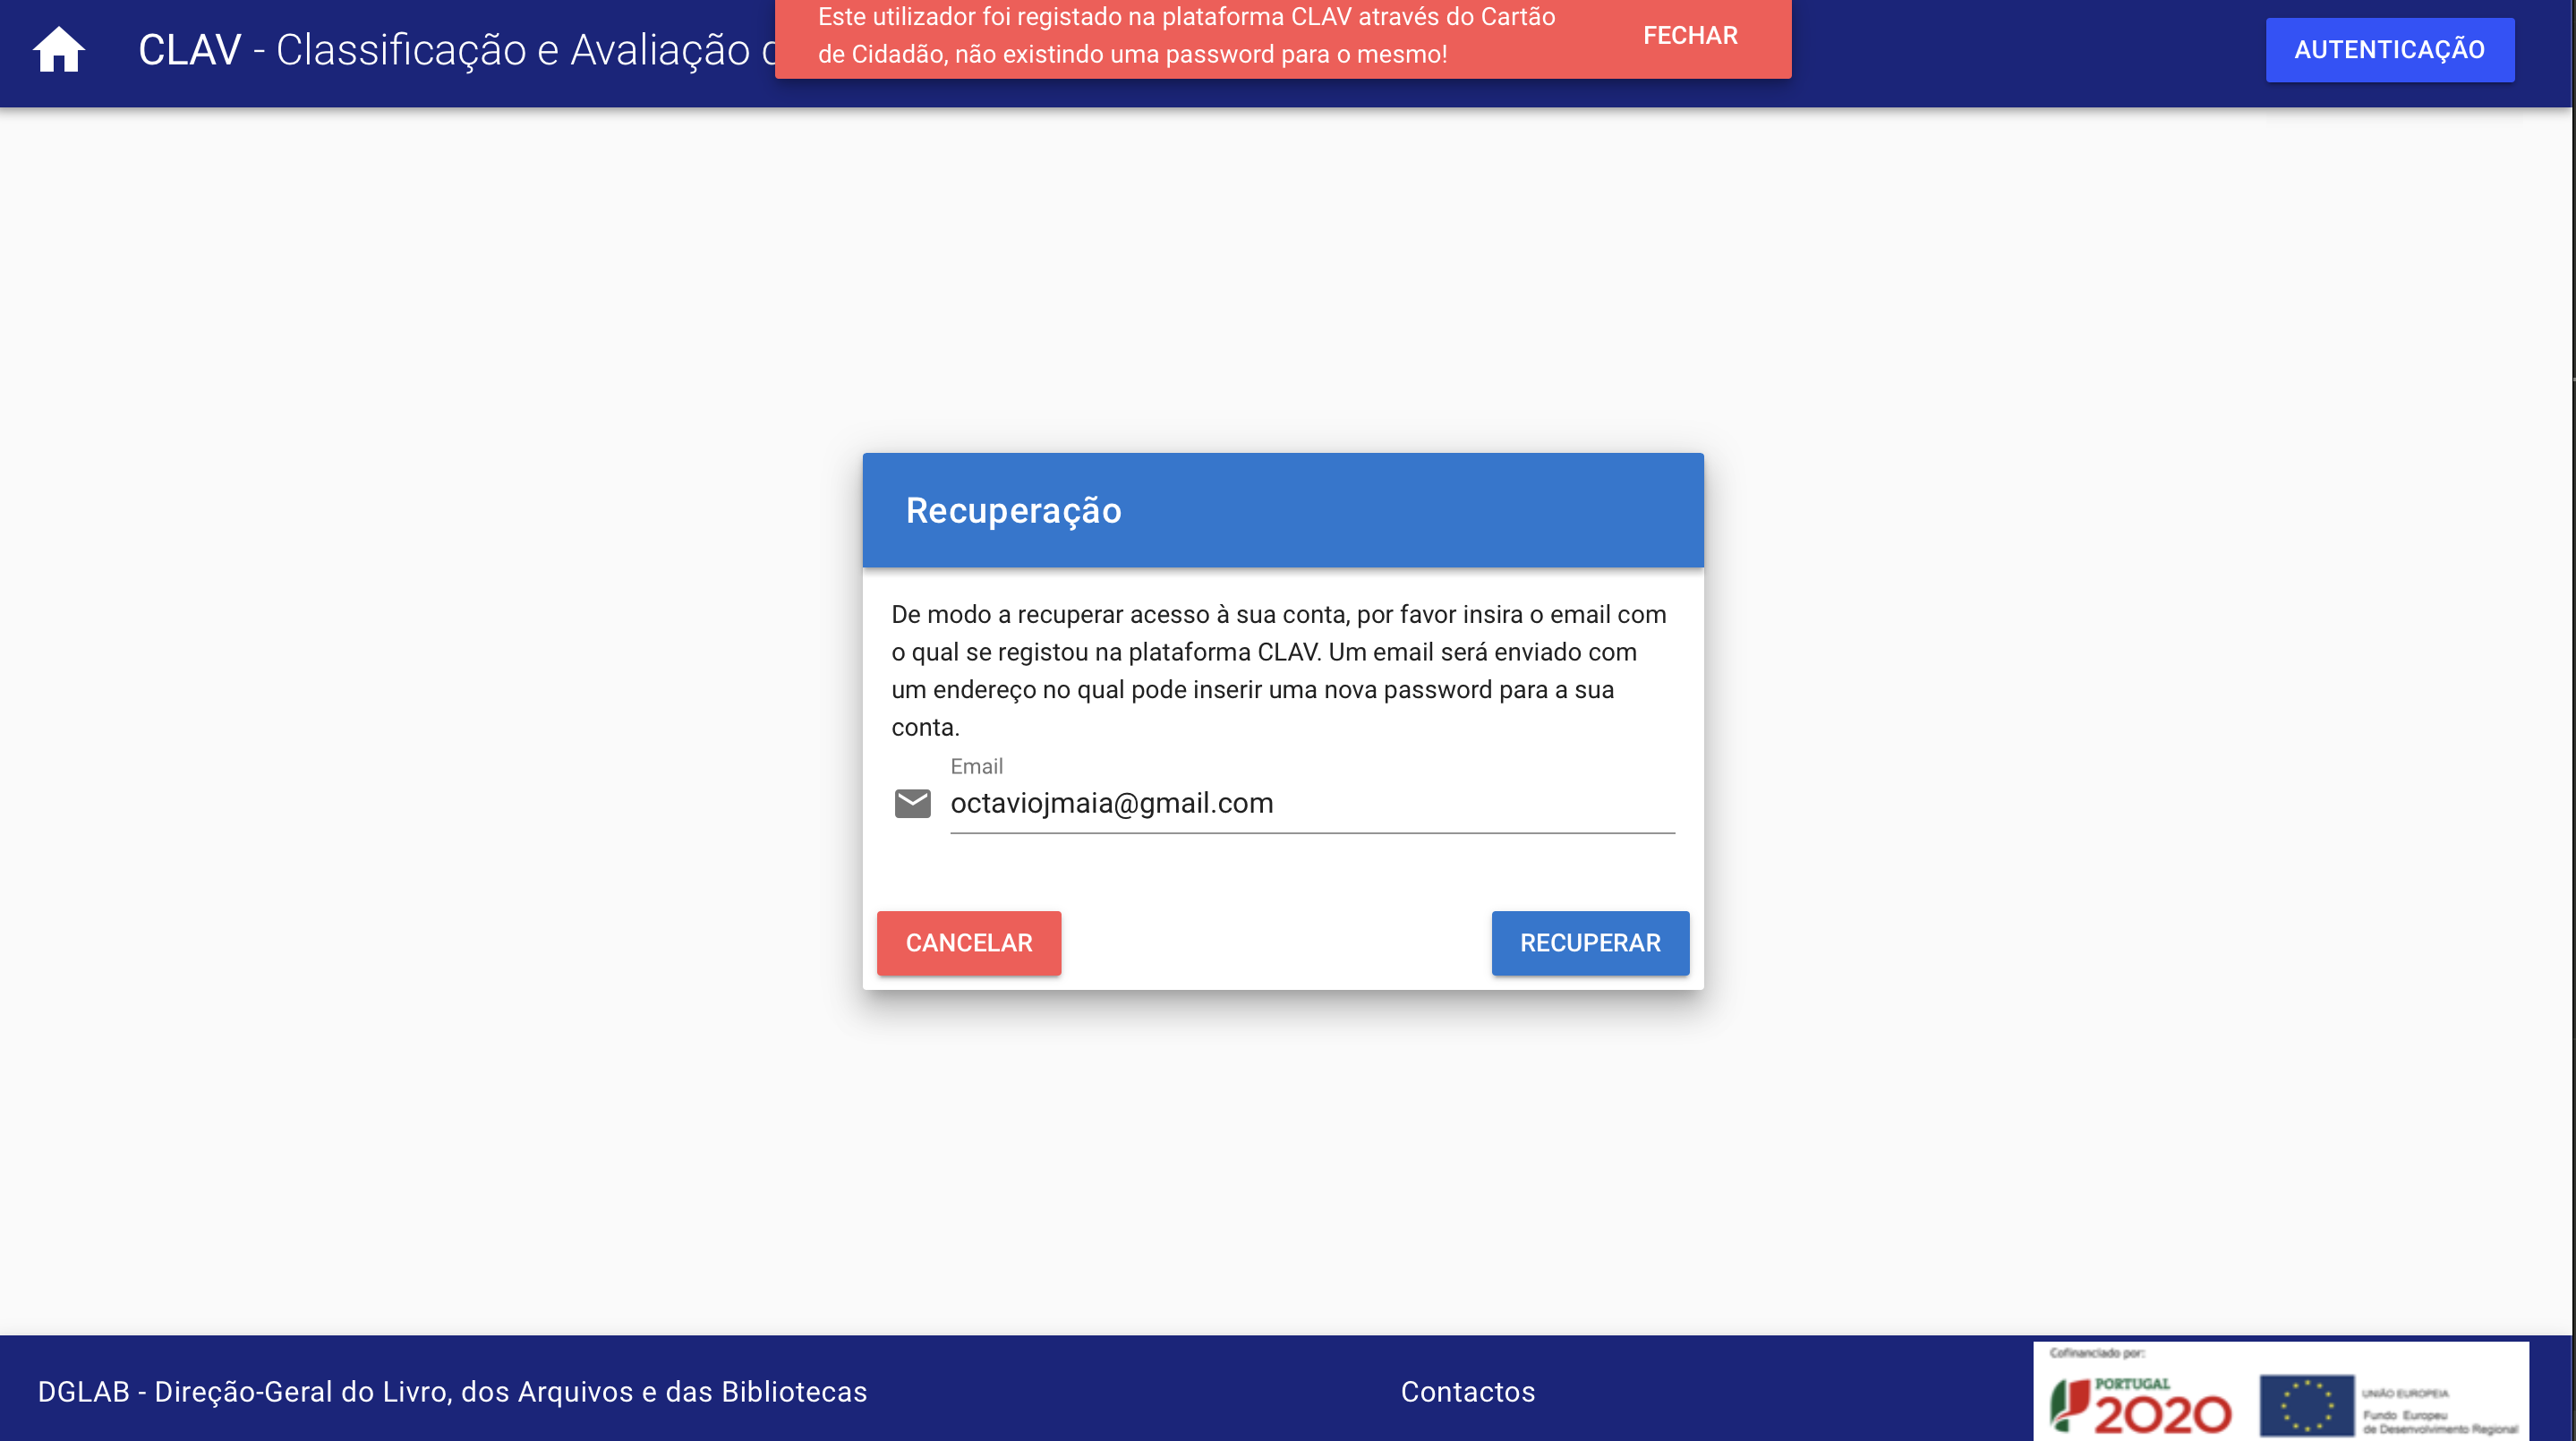
\includegraphics[width=0.9\textwidth]{img/clav/authCC/erroRecuperacao.png}
            \caption{Mensagem de erro após tentativa de recuperação de uma conta registada com Cartão de Cidadão.}
            \label{fig:pagRecuperacaoErroCC}
        \end{figure}
    \end{itemize}
\end{itemize}

O comportamento da função de recuperação pode ser exemplificado pelo seguinte diagrama de sequência:

\vspace{10mm}

\begin{figure}[H]
    \centering
    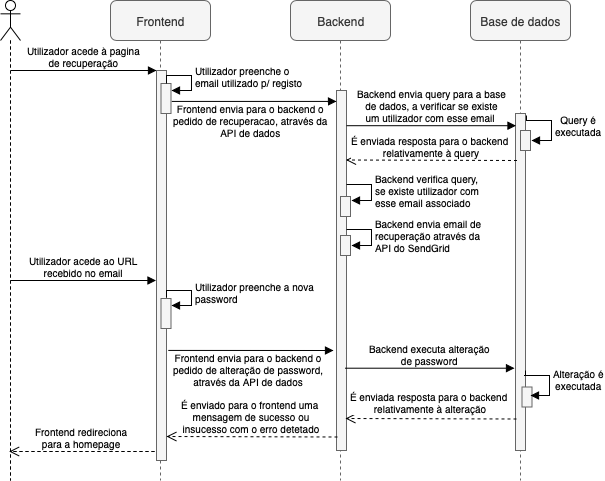
\includegraphics[width=\textwidth]{img/diagramas/sequencia/DiagramasSequencia-Recuperacao.png}
    \caption{Diagrama de sequência relativo ao processo de recuperação na plataforma \gls{clav}.}
    \label{fig:diagramaSequenciaRecuperacao}
\end{figure}

\cleardoublepage
\subsection{Autenticação através de Cartão de Cidadão}

\vspace{-5mm}
Nesta secção iremos explorar a implementação da autenticação com o Cartão de Cidadão através da ferramenta Autenticação.Gov. Iremos começar por relatar o processo de autenticação, seguido do registo de um novo utilizador, bem como o diagrama de sequência deste processo.

Após aceder ao Autenticação.Gov somos abordados com os dados que a plataforma \gls{clav} está a requisitar, tendo este sido abordados na secção \ref{authnRequestSection}.

\vspace{-3mm}
\begin{figure}[H]
    \centering
    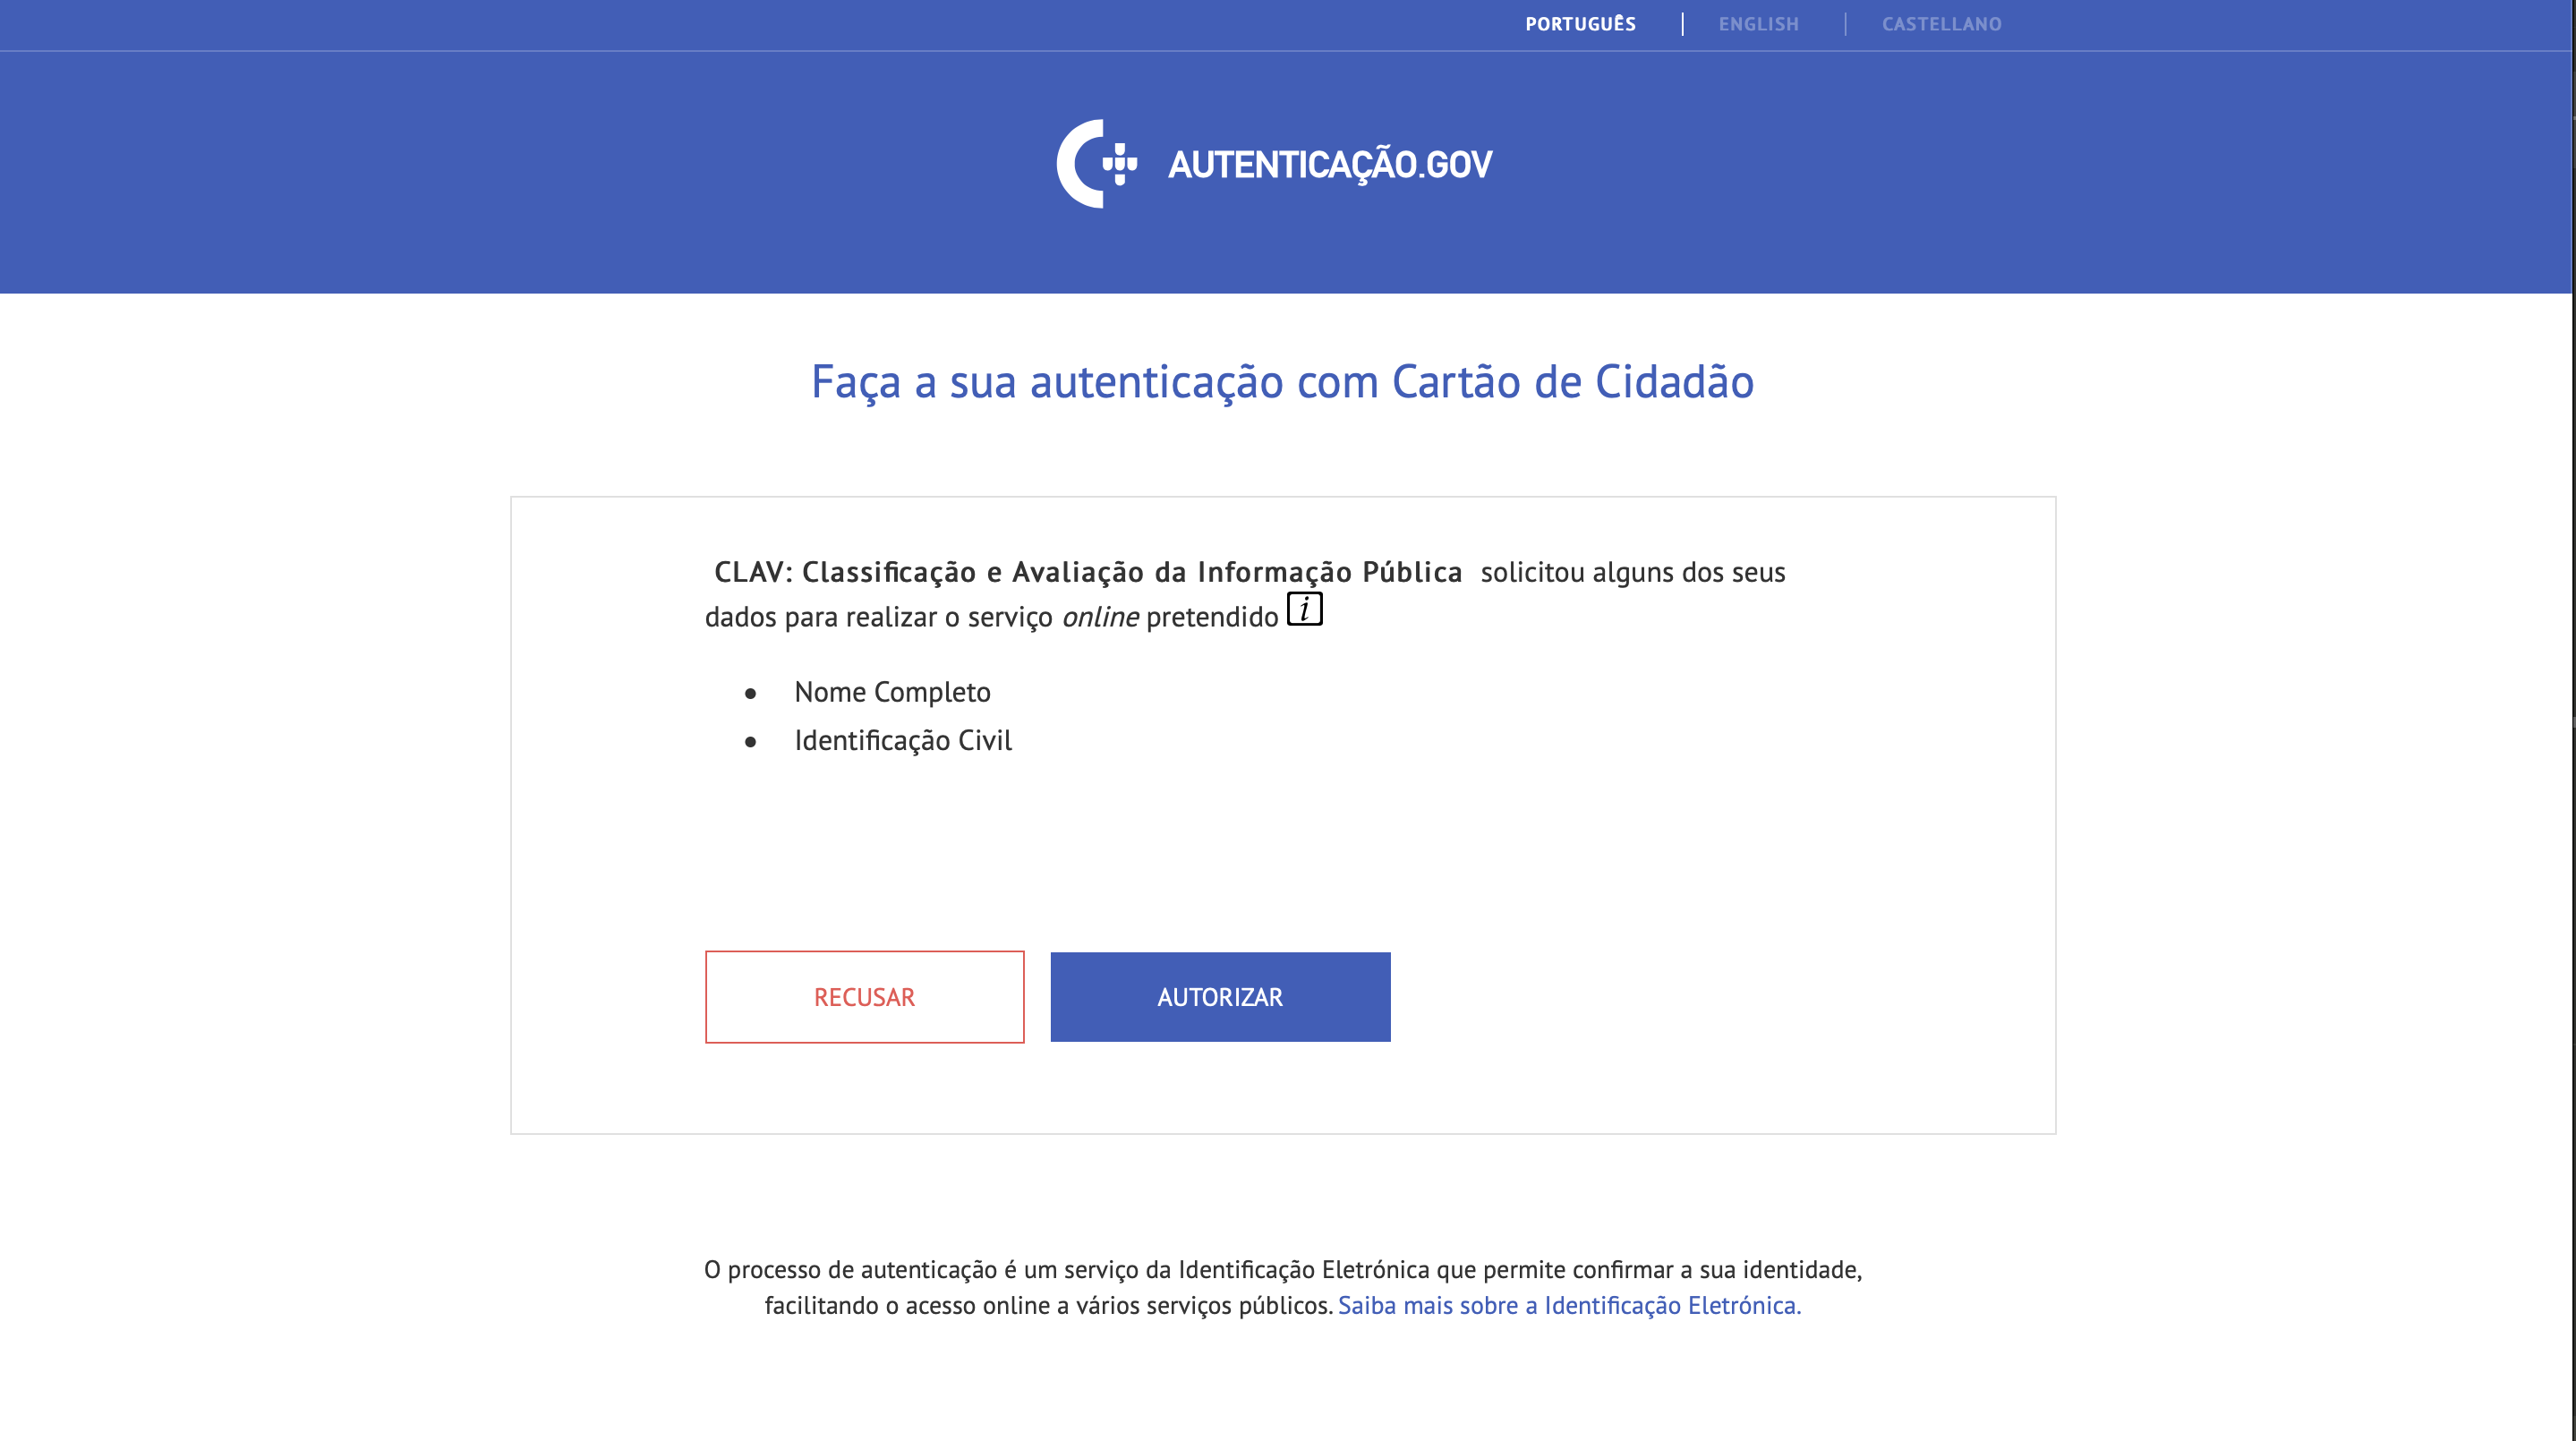
\includegraphics[width=0.9\textwidth]{img/clav/authCC/authgov1.png}
    \caption{Página principal do Autenticação.Gov.}
    \label{fig:landingPageAuthGov}
\end{figure}

\vspace{-3mm}
De seguida é pedido o PIN de autenticação do nosso Cartão de Cidadão.

\vspace{-3mm}
\begin{figure}[H]
    \centering
    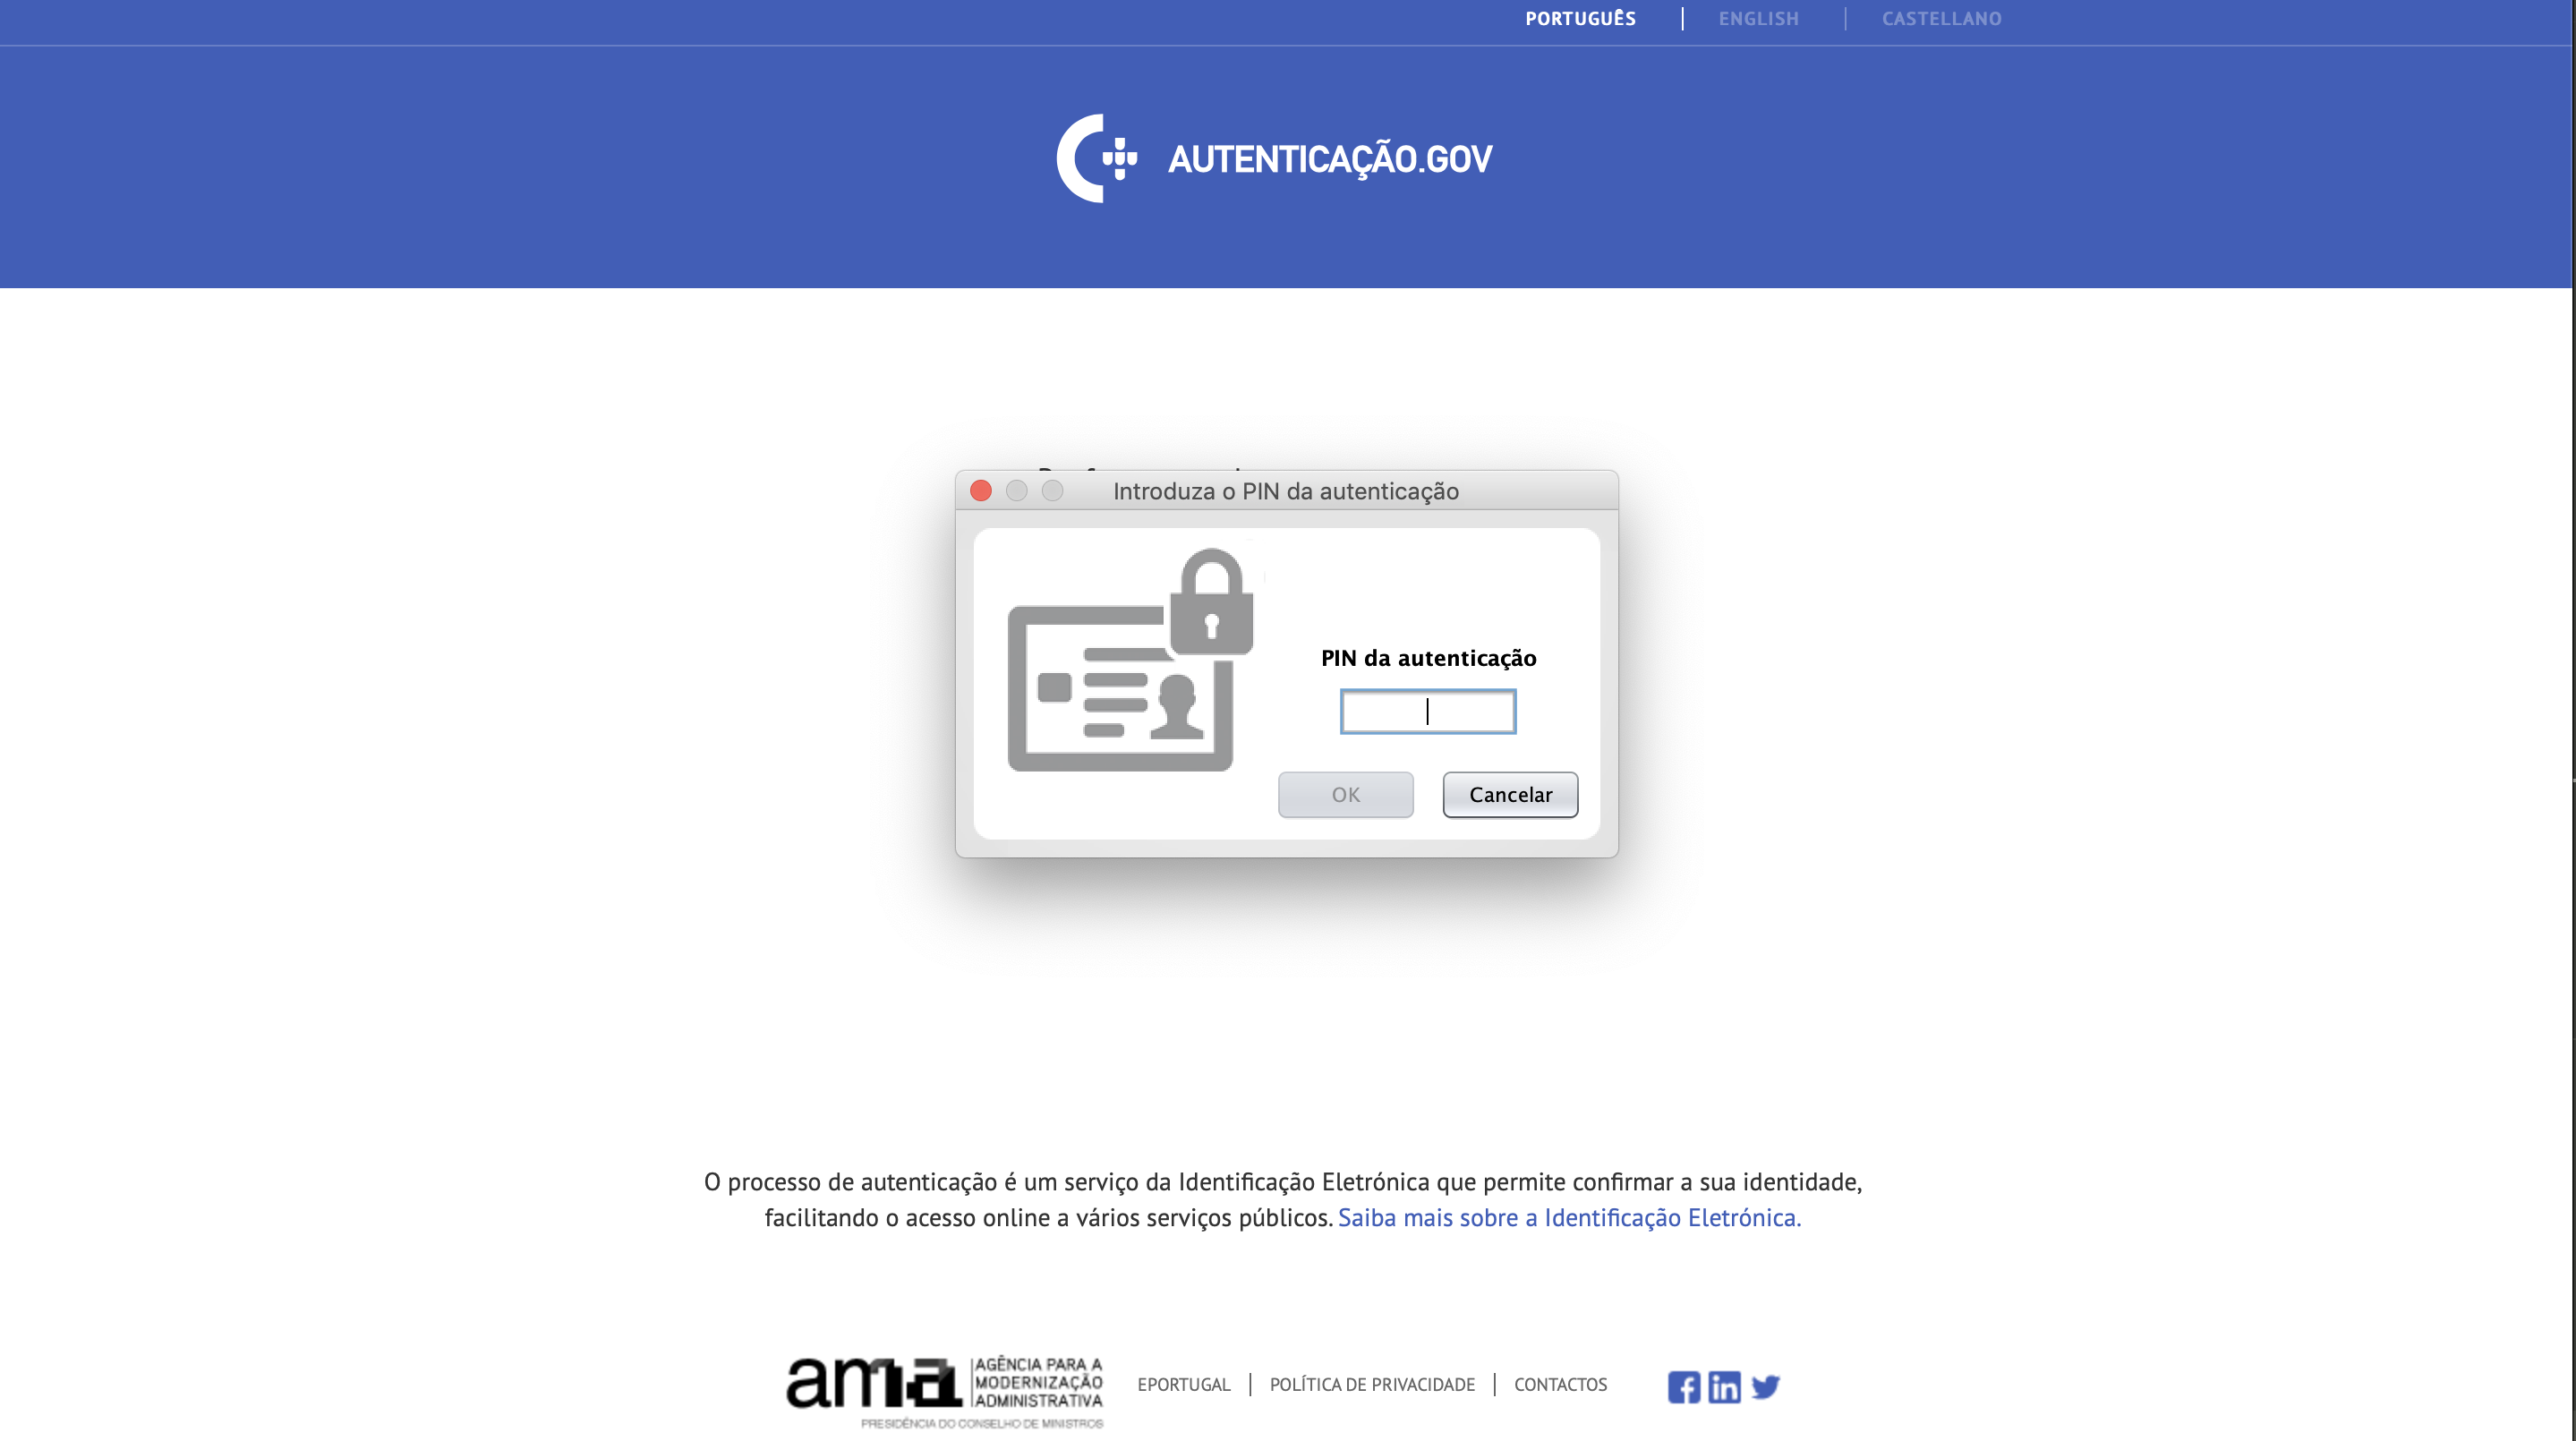
\includegraphics[width=0.9\textwidth]{img/clav/authCC/authgov2.png}
    \caption{Pedido de inserção do PIN de autenticação por parte do Autenticação.Gov.}
    \label{fig:authGovPIN}
\end{figure}

Após esta etapa podem ocorrer dois cenários:

\begin{itemize}
    \item \textbf{Sucesso}
    
    Ocorre quando o utilizador fornece o PIN de autenticação correto.
    
    \begin{figure}[H]
        \centering
        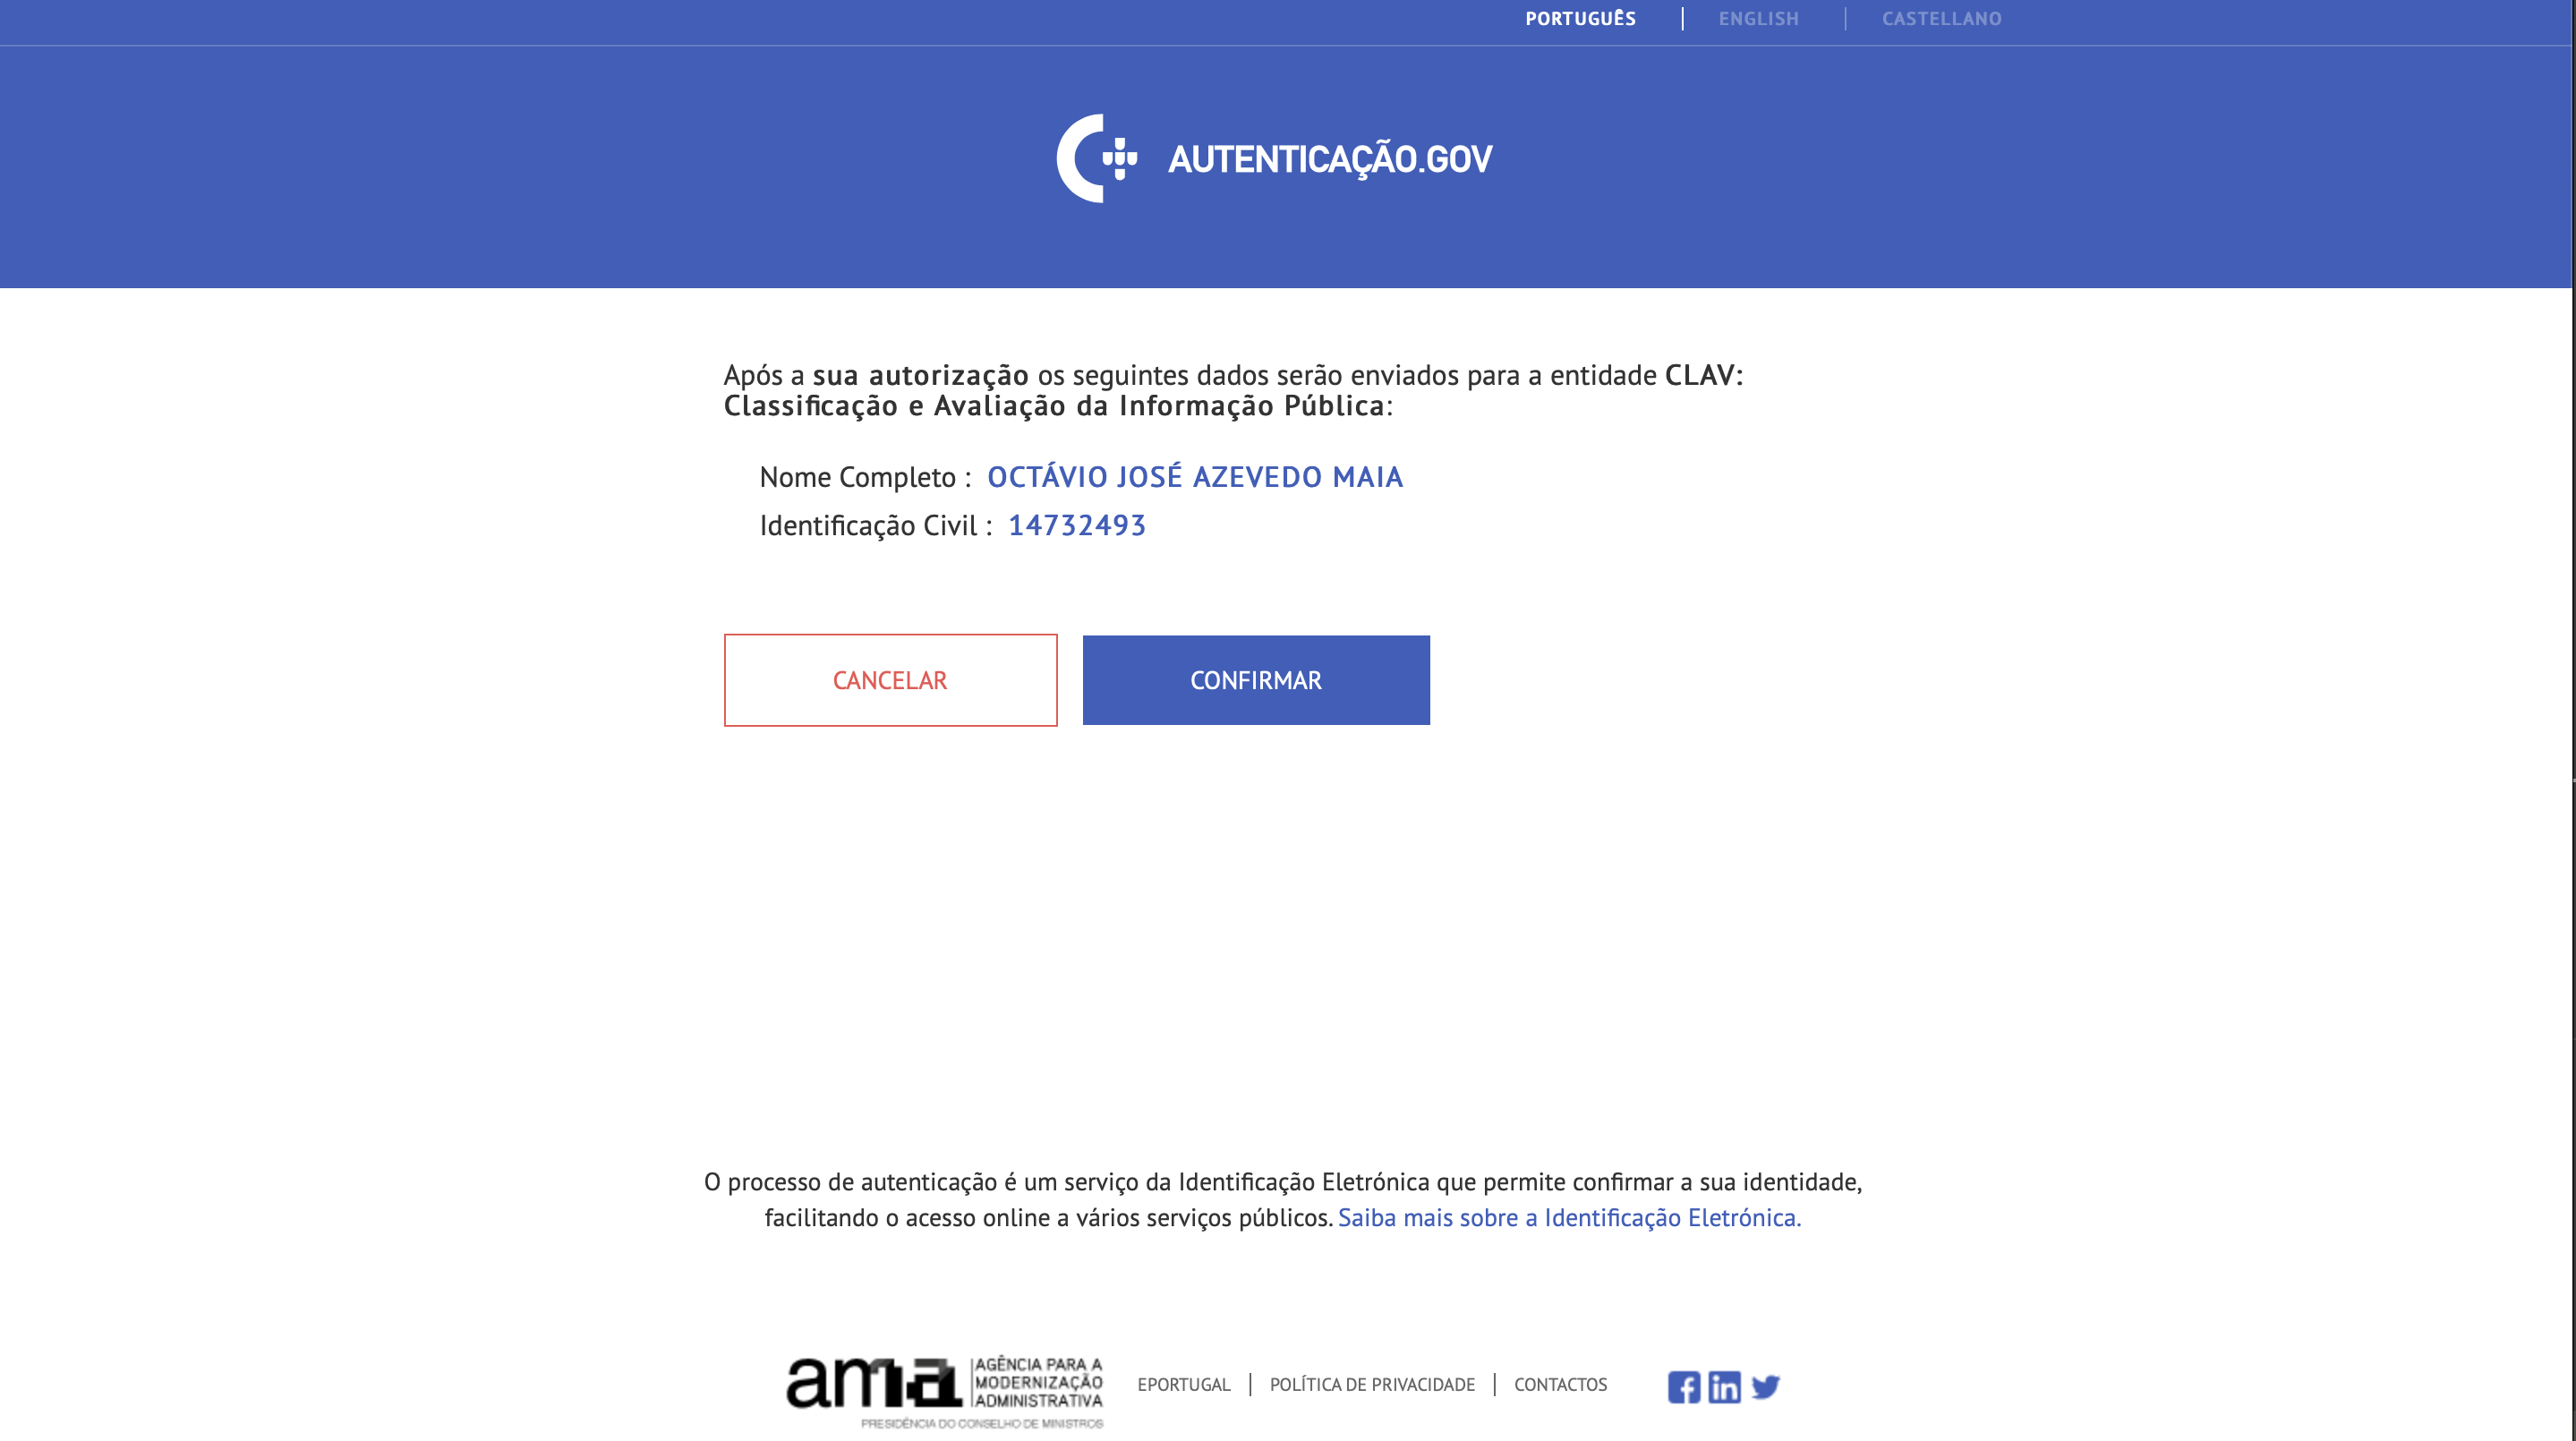
\includegraphics[width=\textwidth]{img/clav/authCC/authgov3.png}
        \caption{Listagem dos dados requisitados pela plataforma \gls{clav}.}
        \label{fig:listagemDadosCLAV}
    \end{figure}
    
    Após correta inserção do PIN de autenticação, é necessário verificar se já existe algum utilizador registado com o Número de Identificação Civil (\gls{nic}) devolvido pelo Autenticação.Gov.
    
    \begin{itemize}
        \item \textbf{Já existe utilizador registado}
        
        É iniciada a sessão com o utilizador correspondente a esse \gls{nic} seguido do redireccionamento do utilizador para a página principal.
            
        \vspace{10mm}
        \item \textbf{Não existe utilizador registado}
        
        É feito o redireccionamento para a página de registo de um novo utilizador.
        
        \begin{figure}[H]
            \centering
            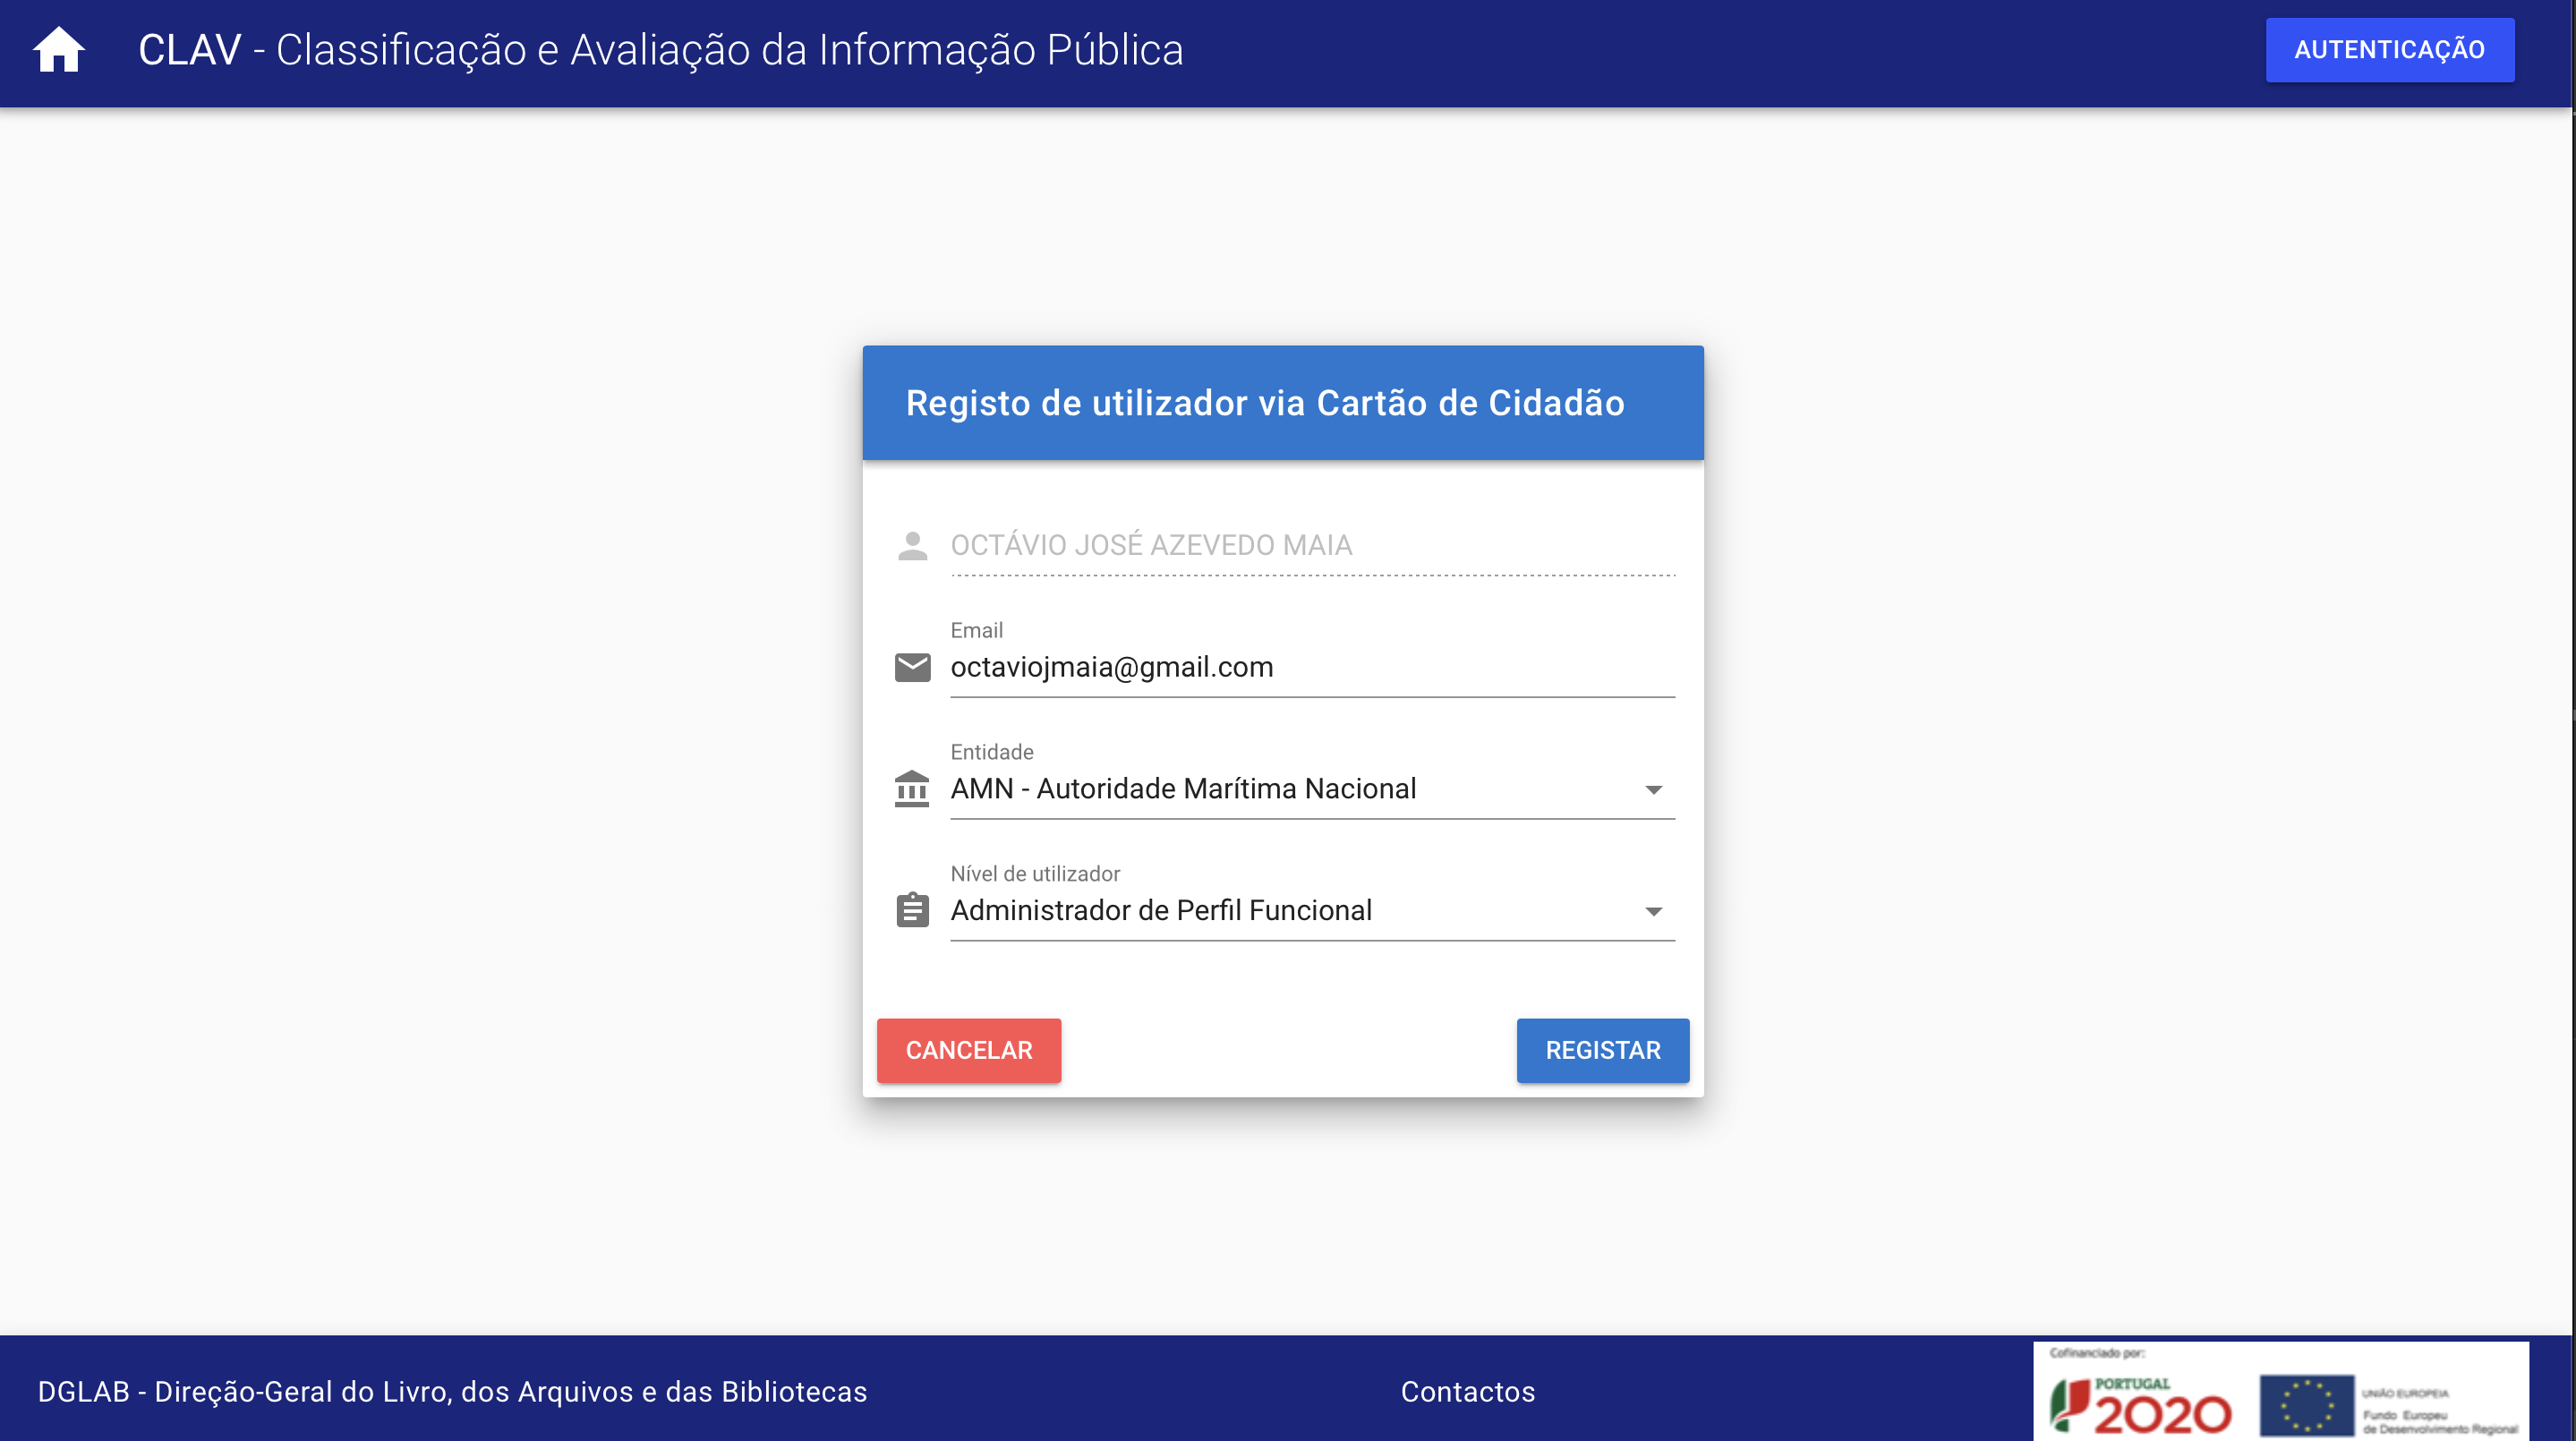
\includegraphics[width=\textwidth]{img/clav/authCC/registo.png}
            \caption{Página de registo de um novo utilizador através do Cartão de Cidadão.}
            \label{fig:pagRegistoCC}
        \end{figure}
    \end{itemize}
    
    \item \textbf{Insucesso}
    
    Ocorre quando o utilizador introduziu um PIN de autenticação incorreto ou negou o acesso à informação requisitada.
    
    \begin{figure}[H]
        \centering
        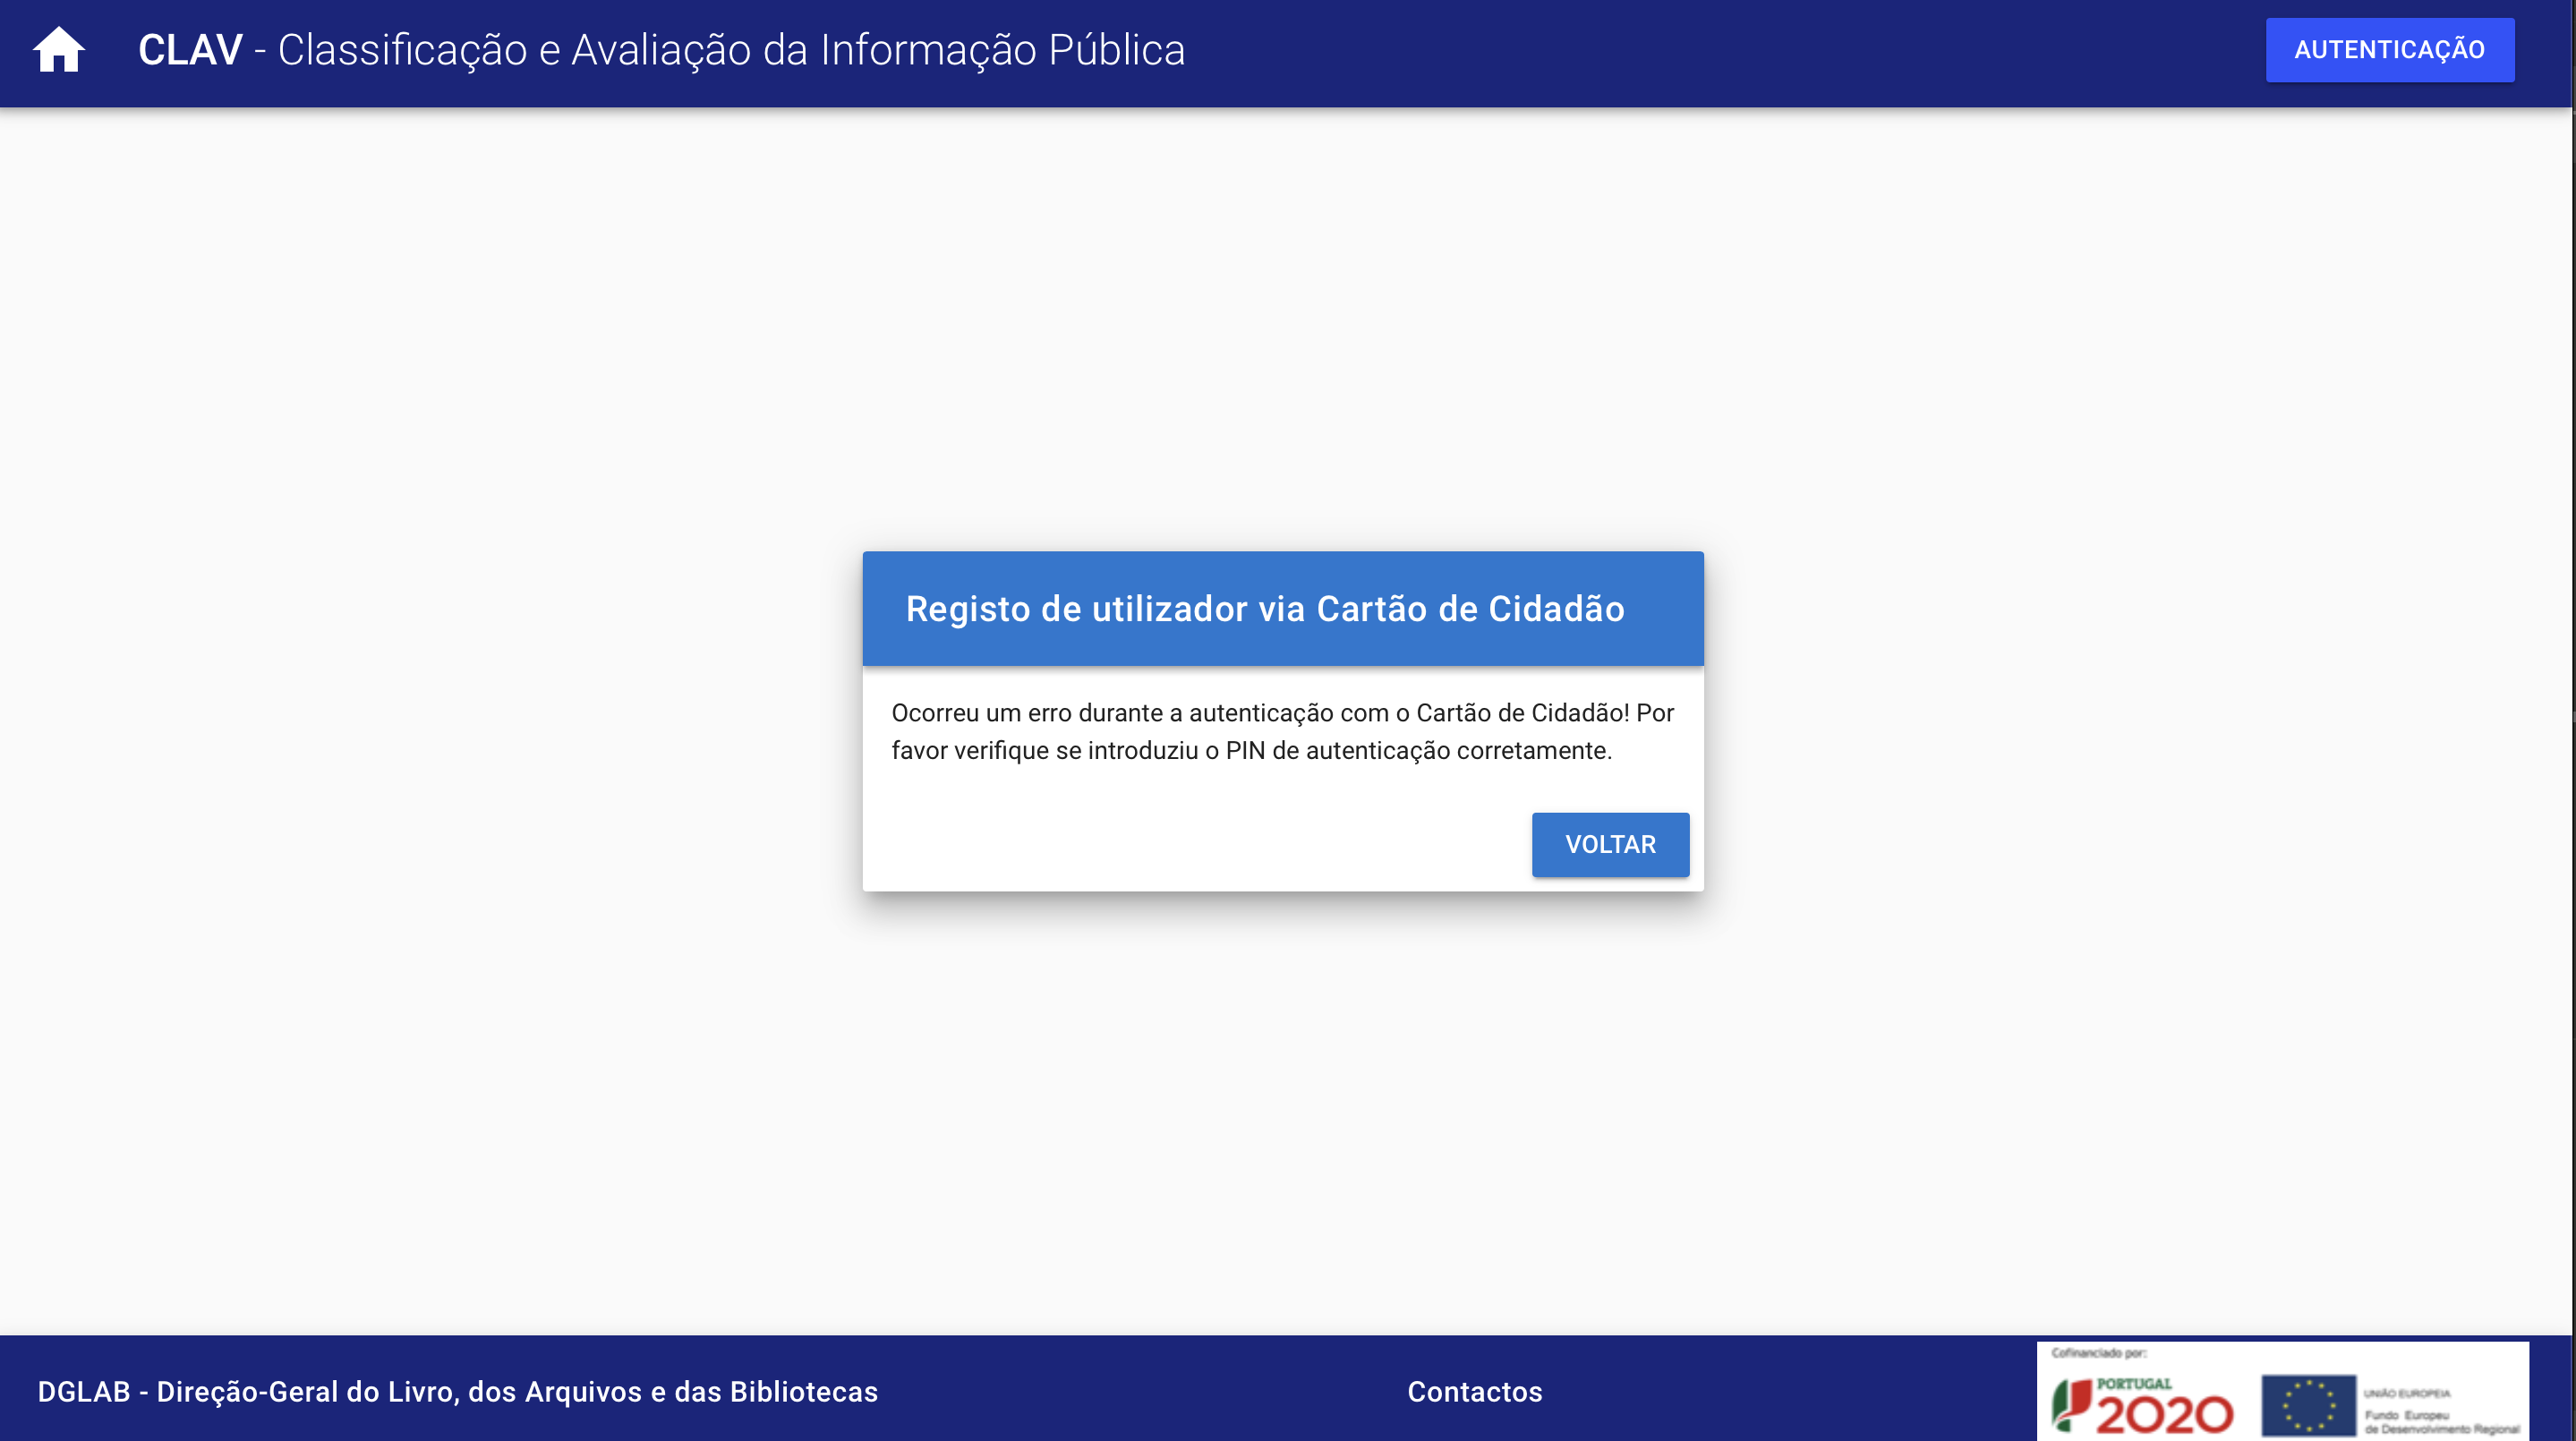
\includegraphics[width=\textwidth]{img/clav/authCC/erroCC.png}
        \caption{Página de erro resultante de um PIN incorreto ou negação da leitura dos dados pretendidos.}
        \label{fig:pagRecuperacaoErroCC}
    \end{figure}
\end{itemize}

O comportamento da função de registo e login via Cartão de Cidadão pode ser exemplificado pelo seguinte diagrama de sequência:

\vspace{5mm}
\begin{figure}[H]
    \centering
    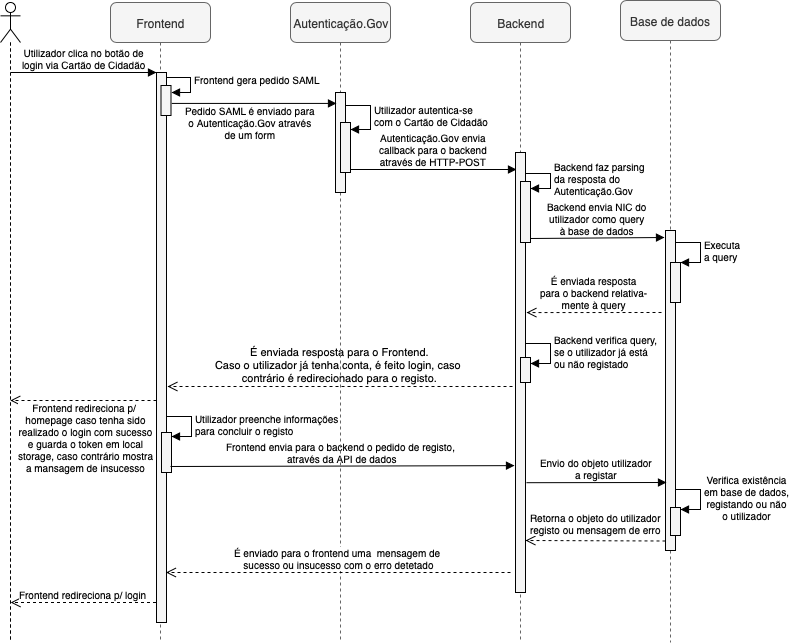
\includegraphics[width=\textwidth]{img/diagramas/sequencia/DiagramasSequencia-LoginCC.png}
    \caption{Diagrama de sequência relativo ao processo de registo e login através de Cartão de Cidadão na plataforma \gls{clav}.}
    \label{fig:diagramaSequenciaCC}
\end{figure}

\cleardoublepage
\subsection{Armazenamento e validação de sessões}

De modo a fazer uma gestão de utilizadores mais aprofundada, foi necessário implementar métodos capazes de não só limitar o número de utilizadores ativos a cada dado momento, mas também manter as sessões iniciadas no caso de falha do servidor.

Numa primeira fase do projeto \gls{clav} foi implementada uma solução baseada em \emph{JSON Web Token}, que será explicada na subsecção \ref{jwt_1}. Embora esta se tenha provado eficaz, a mesma não era capaz de manter as sessões iniciadas no caso de uma falha súbita do servidor, ou seja, se o servidor por algum motivo sofresse de uma falha de energia e tivesse de reiniciar, devido às sessões estarem guardadas localmente, as mesmas eram perdidas.

Outro fator decisivo contra esta implementação assenta no facto de não ser possível recorrer ao paralelismo da aplicação através do \emph{nginx}\footnote{Mais informação em \url{https://www.nginx.com}}, pois a comunicação entre processos paralelos não permite a partilha do token guardado localmente.

Para tal, foi necessário recorrer a outra abordagem, o armazenamento de sessões em base de dados, neste caso em \emph{MongoDB}.

Esta segunda implementação em \emph{MongoDB}, embora totalmente funcional, teria de ser abandonada devido à divisão da aplicação especificada no capítulo \ref{implementacao}. Assim sendo, as secções \ref{jwt_1} e \ref{armazenamentoMongo} podem ser encaradas como processos iterativos na cadeia de desenvolvimento da plataforma \gls{clav}, sendo a secção \ref{jwt_2} representativa do estado atual do projeto.

\subsubsection{Validação através de JSON Web Token} \label{jwt_1}

Durante o desenvolvimento do projeto \gls{clav} foi discutida a implementação de um mecanismo capaz de terminar sessões automaticamente, de modo a diminuir o número de sessões ativas, bem como evitar possíveis falhas de segurança.

Para tal foi implementado, juntamente com o \emph{Passport}, uma estratégia capaz de lidar com \gls{jwt}, representada através do seguinte pseudo código.

\begin{algorithm}
    \caption{Pseudo código da autenticação via \emph{JSON Web Token}.}
    \begin{algorithmic}[1]
        \Function{JwtStrategy}{opts, jwt\_payload, done}
        \State $user \gets findUserByJwt(jwt\_payload.id)$
        \If {$user \neq invalid$}
            \State \textbf{return} done(null, user)
        \Else
            \State \textbf{return} done(null, false)
        \EndIf
    \EndFunction
    \end{algorithmic}
\end{algorithm}

Através do uso do \emph{JSON Web Token}, é possível povoar o atributo \emph{exp} com uma data de expiração, após a qual o token se torna inválido, terminando assim a sessão do utilizador.

Para tal, quando a estratégia de login local do \emph{Passport} é invocada, é necessário proceder à assinatura de um token \gls{jwt} e atribuí-lo à sessão do utilizador atual.

\begin{algorithm}
    \caption{Pseudo código da atribuição de um \gls{jwt} à sessão.}
    \label{algoritmoJWT1}
    \begin{algorithmic}[1]
        \Function{login}{user}
        \State $token \gets jwt.sign({user}, jwt.secret, \{$
        \State \indent $expiresIn : jwt.expiration$
        \State $\}$
        \State $session.token \gets token$
    \EndFunction
    \end{algorithmic}
\end{algorithm}

Os valores de \emph{secret} e \emph{expiration} previamente utilizados são provenientes de um ficheiro externo, no qual designamos a duração (em segundos) em que a sessão está ativa, bem como a chave secreta utilizada para a assinatura.

\begin{verbatim}
    jwt: {
        secret: 'ihfH6Cv4LVD1YoG...vY8XdVch5ebGHTdPMDGHy',
        expiration: 3000 //in seconds
    }
\end{verbatim}

Após corretamente atribuída a sessão a um utilizador, cada vez que o mesmo pretende aceder a páginas restritas, como por exemplo, a adição de entidades à plataforma \gls{clav} é realizada uma chamada ao \emph{middleware} de autenticação \emph{isLoggedIn}, o qual verifica se existe um utilizador com sessão iniciada, bem como se o token do mesmo ainda não expirou, sendo esta lógica representada através do seguinte pseudo código.

\begin{algorithm}
    \caption{Pseudo código da função  de middleware \emph{isLoggedIn}.}
    \begin{algorithmic}[1]
        \Function{isLoggedIn}{req, res, next}
        \If {$req.isAuthenticated()$}
        \State $result \gets jwt.verify(session.token, jwt.secret)$
            \If {$result \neq expired$}
                \State \textbf{return} next()
            \Else
                \State \textbf{return} err
            \EndIf
        \EndIf
    \EndFunction
    \end{algorithmic}
\end{algorithm}

Embora esta implementação do \emph{JSON Web Token} estivesse 100\% funcional, a mesma foi abandonada da gestão de utilizadores por uma alternativa similar, o armazenamento de sessões ativas diretamente na base de dados em \emph{MongoDB}, sendo apenas utilizado o \gls{jwt} na autenticação de pedidos à \gls{api}.

\cleardoublepage
\subsubsection{Armazenamento em MongoDB} \label{armazenamentoMongo}

O armazenamento de sessões em \emph{MongoDB} permite uma maior flexibilidade comparativamente com o armazenamento local.

Em primeiro lugar é possível recorrer ao paralelismo da aplicação via \emph{nginx} ou outras soluções similares, pois cada \emph{thread} pode correr independentemente umas da outras e a comunicação entre processos paralelos passa a ser inexistente. Para validar sessões cada \emph{thread} faz uma \emph{query} à base de dados, verificando se a sessão do utilizador é válida.

Permite também que na ocorrência de uma falha súbita do sistema, as informações relativas às sessões não se percam devido a estarem armazenadas em base de dados. Assim sendo, após o \emph{boot} do sistema, os utilizadores continuam com as sessões ativas, algo que não aconteceria se fosse utilizado armazenamento local e validação via \gls{jwt}.

Um possível problema desta solução seria que iríamos delegar o armazenamento das sessões para o lado do servidor, ou seja, se por ventura existissem milhões de sessões armazenadas, iria ser ocupado um tamanho substancial de memória em disco. Para evitar tal problema, é utilizado o módulo \emph{\textbf{connect-mongo}}\footnote{\url{https://github.com/jdesboeufs/connect-mongo}} que permite a auto remoção de sessões expiradas, bem como a atribuição de um tempo máximo após o qual a sessão expira.

Para atingir este objetivo, apenas é necessário adicionar os campos abaixo mencionados à sessão do \emph{ExpressJS}.

\begin{verbatim}
    app.use(session({
        ...
        autoRemove: 'interval',
        autoRemoveInterval: 15, //minutes
        store: new MongoStore({
            url: dataBases.userDB,
            ttl: 1800 //seconds
        })
    }));
\end{verbatim}

Esta configuração do módulo \emph{\textbf{connect-mongo}} faz com que a cada 15 minutos seja invocada a função de remoção de sessões expiradas, sendo que cada sessão apenas é válida durante 1800 segundos, ou seja, 30 minutos.

Em suma, o armazenamento de sessões em base de dados possui todas as qualidades da validação via \emph{JSON Web Token}, oferecendo uma maior flexibilidade e customização, sem impacto na performance do servidor.

\cleardoublepage
\subsubsection{Nova técnica de validação através de JSON Web Token} \label{jwt_2}

Devido à separação do frontend e backend em aplicações distintas, explicada na secção \ref{implementacao}, a existência de uma sessão em base de dados deixa de ser possível. Isto deve-se ao facto do utilizador ter de iniciar sessão no servidor responsável pelo frontend da aplicação, sendo os dados introduzidos enviados para o backend, seguido da resposta do mesmo para o frontend (explicado na figura \ref{fig:diagramaLogin}).

Devido ao envio da informação para outro servidor, esta informação e posterior sessão são armazenadas no servidor do backend e não do frontend. Caso a separação do frontend e backend não tivesse ocorrido, ambos correriam no mesmo servidor e este problema não existiria.

Para tal, foi necessário implementar um novo método de validação de sessões, fortemente baseado na autenticação em tokens discutida na secção \ref{jwt_1}.

A função de login foi alterada de modo a enviar os seguintes parâmetros:

\begin{itemize}
    \item \textbf{Token \gls{jwt}}
    
    Em vez de guardar toda a informação do utilizador como o algoritmo \ref{algoritmoJWT1} foi decidido que este iria apenas conter o ID do utilizador, sendo realiza uma query à base de dados quando é necessário obter informações sobre o mesmo (o token criado possui 8h de validade).
    
    Este comportamento pode ser exemplificado pelo algoritmo \ref{algoritmoJWT2}.
    
    \begin{algorithm}
        \caption{Pseudo código da atribuição de um \gls{jwt} à sessão.}
        \label{algoritmoJWT2}
        \begin{algorithmic}[1]
            \Function{login}{user}
            \State $token \gets jwt.sign({id: user._id}, jwt.secret, \{$
            \State \indent $expiresIn : 8h$
            \State $\}$
            \State $name \gets user.name$
            \State $entidade \gets user.entidade$
            \State $res.send(token,name,entidade)$
        \EndFunction
        \end{algorithmic}
    \end{algorithm}
        
    \item \textbf{Nome do utilizador.}
    
    %Este parâmetro é utilizado para atribuir o nome do utilizador cuja sessão está iniciada na plataforma \gls{clav}.
    
    \item \textbf{Entidade do utilizador.}
\end{itemize}

Ao receber o token \gls{jwt}, o nome e a entidade do backend, estes são guardados em local storage através do \emph{Vuex Store}. Sempre que uma página é acedida, é verificado se o token ainda não expirou de modo a terminar automaticamente as sessões.

Com esta nova técnica de validação e armazenamento de sessões através de tokens \gls{jwt} é possível separar as aplicações em servidores distintos, mantendo também a sessão iniciada em caso de falha de servidor.

\cleardoublepage
\section{Autenticação de pedidos à API de dados}

Nesta secção iremos explorar a implementação da autenticação de pedidos realizados à API de dados descrita na secção \ref{protecaoAPI}.

A API de dados da plataforma \gls{clav} foi desenvolvida com o intuito de fornecer uma API pública, sem autenticação, e outra carente de autenticação, a ser utilizada por fornecedores de serviços que queiram desenvolver aplicações ou outros serviços que requerem a obtenção de dados da plataforma.

Assim sendo, nesta secção iremos analisar a página de registo de uma chave API para os fornecedores de serviços, bem como a renovação da mesma, e como esta autenticação é processada no backend.

\subsection{Registo} \label{registoChaveApi}
\begin{figure}[H]
    \centering
    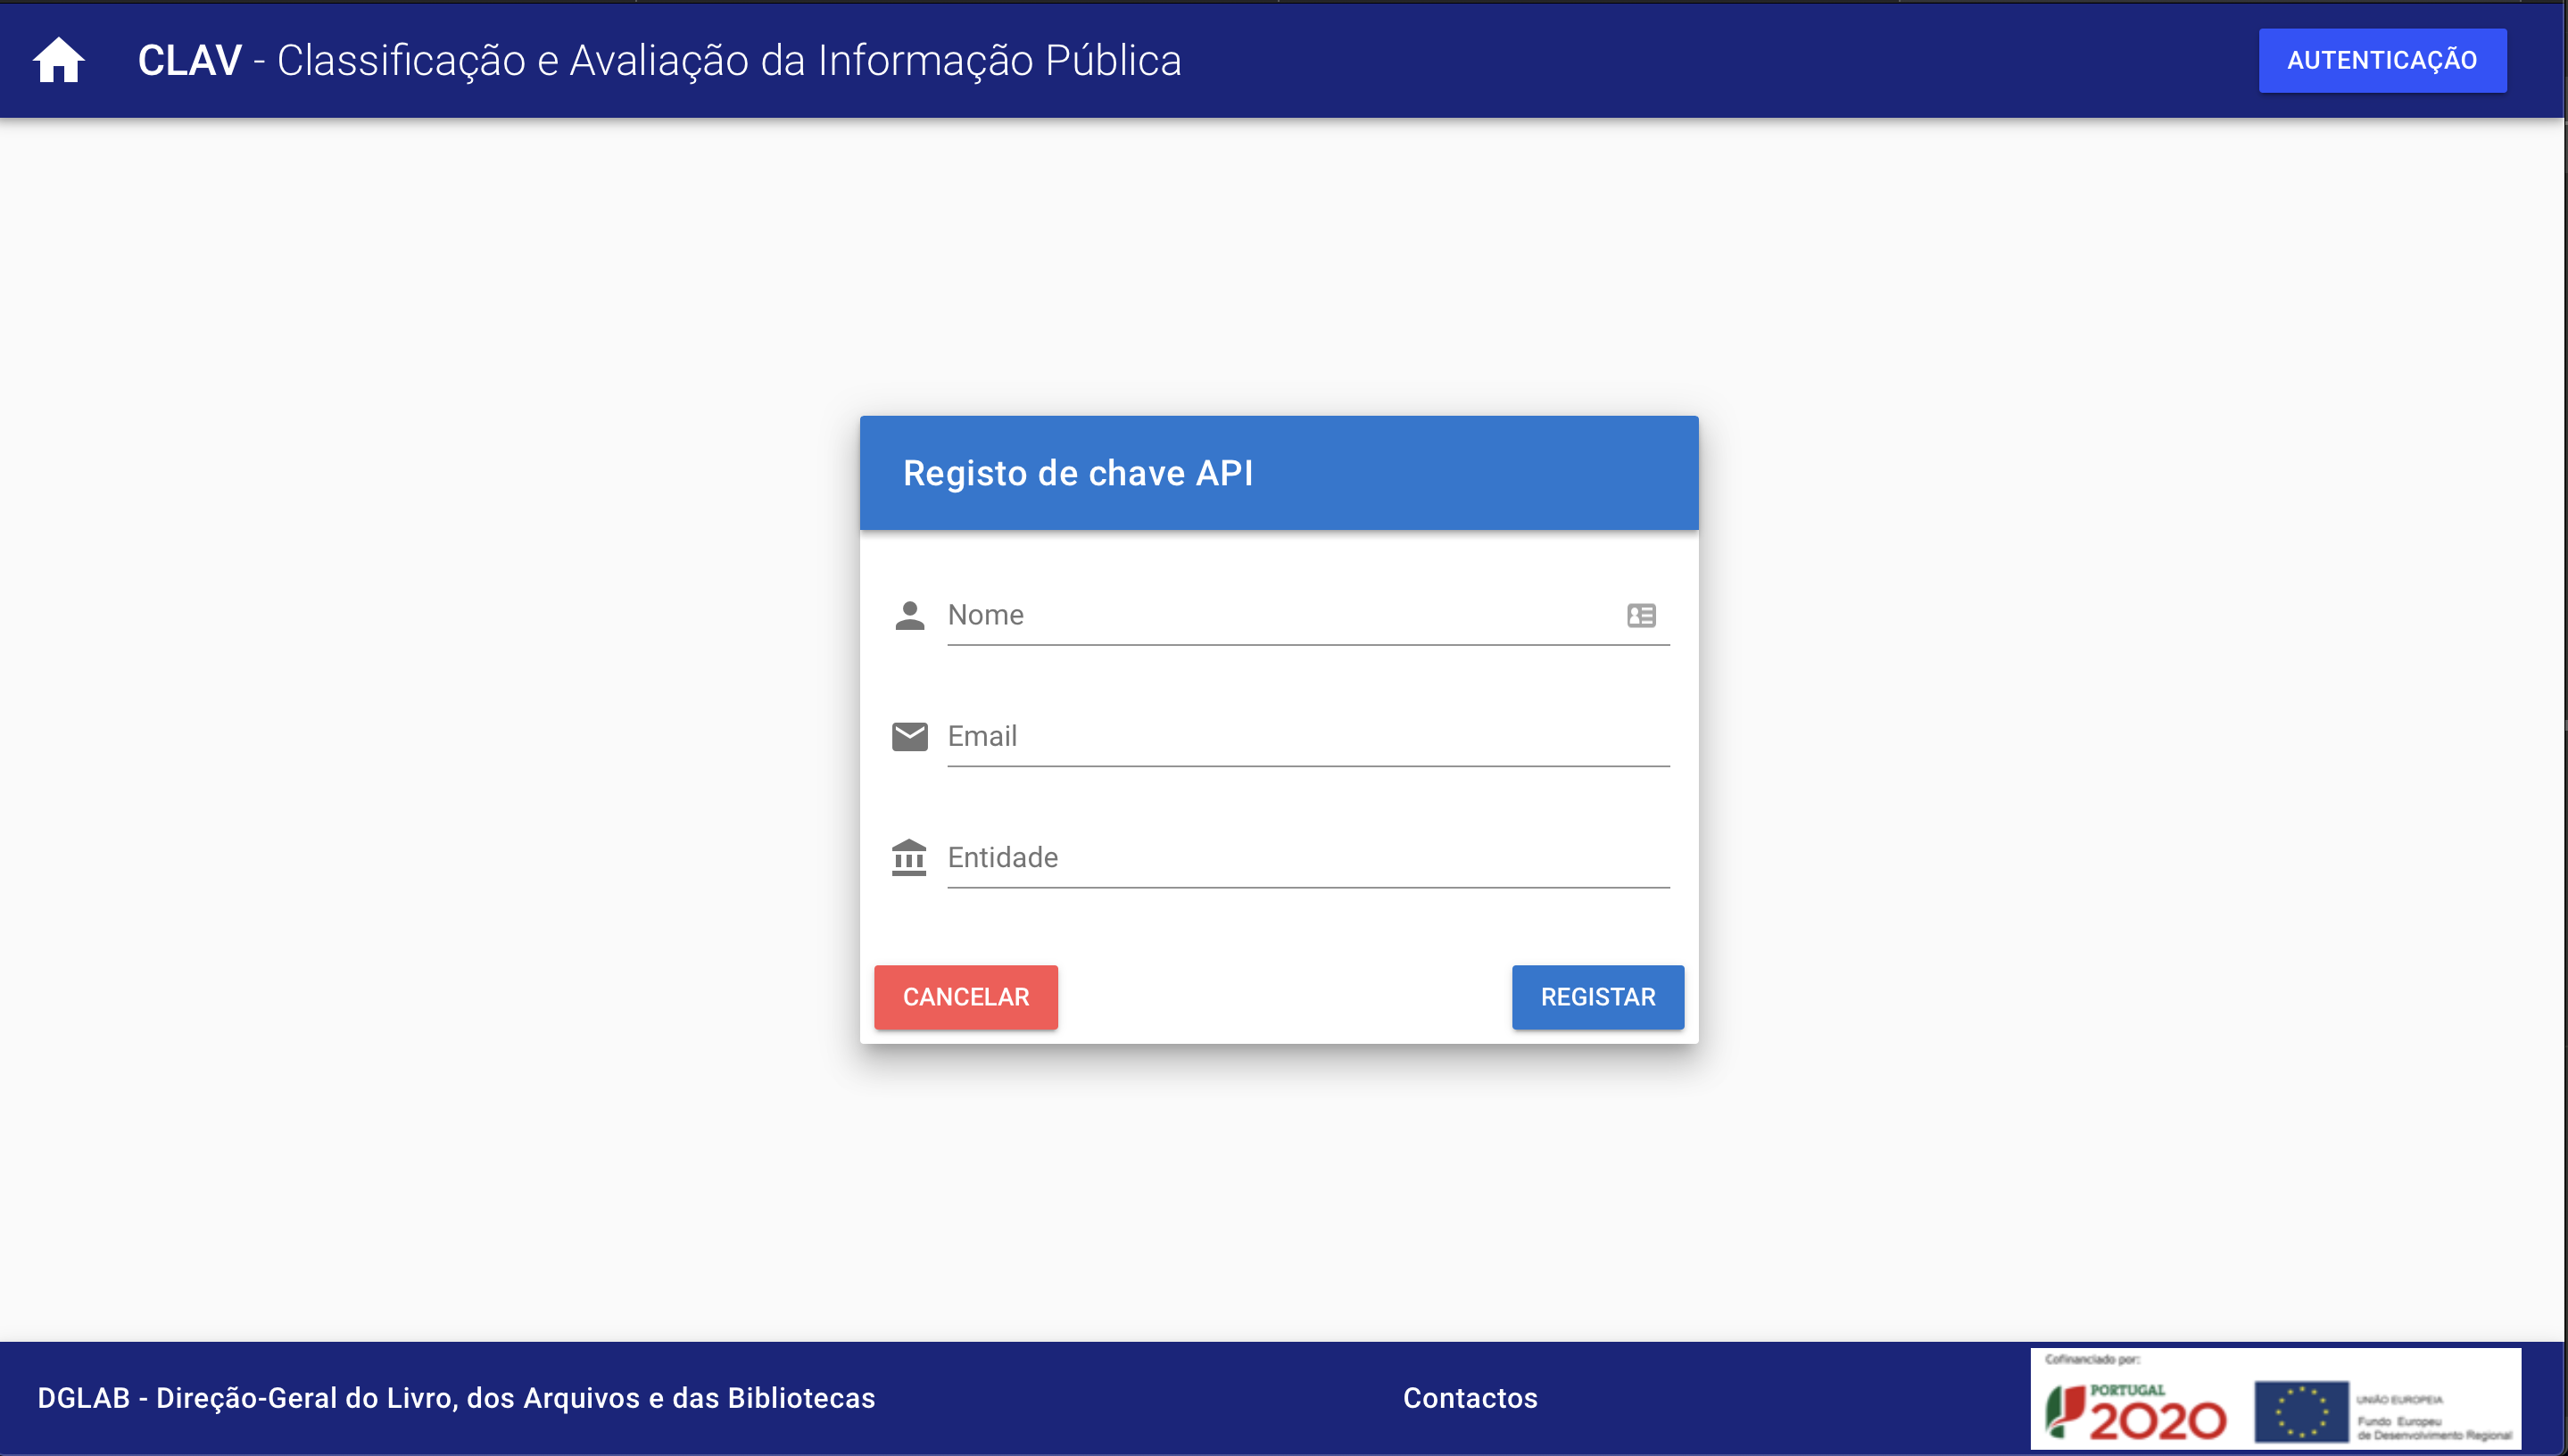
\includegraphics[width=0.95\textwidth]{img/clav/authAPI/registar.png}
    \caption{Página de registo de uma chave API na plataforma \gls{clav}.}
    \label{fig:registoChaveAPI}
\end{figure}

O registo de uma chave API por parte de um fornecedor de serviços requer o preenchimento da seguinte informação:

\begin{enumerate}
    \item Nome.
    \item Email (este tem de ser válido de modo a permitir a renovação da chave API).
    \item Entidade (informação da entidade que está a requisitar a chave API).
\end{enumerate}

Após submeter o pedido de registo de uma chave API é enviado para o email especificado a informação relativa à chave API emitida para a entidade/fornecedor de serviços em questão.

\begin{figure}[H]
    \centering
    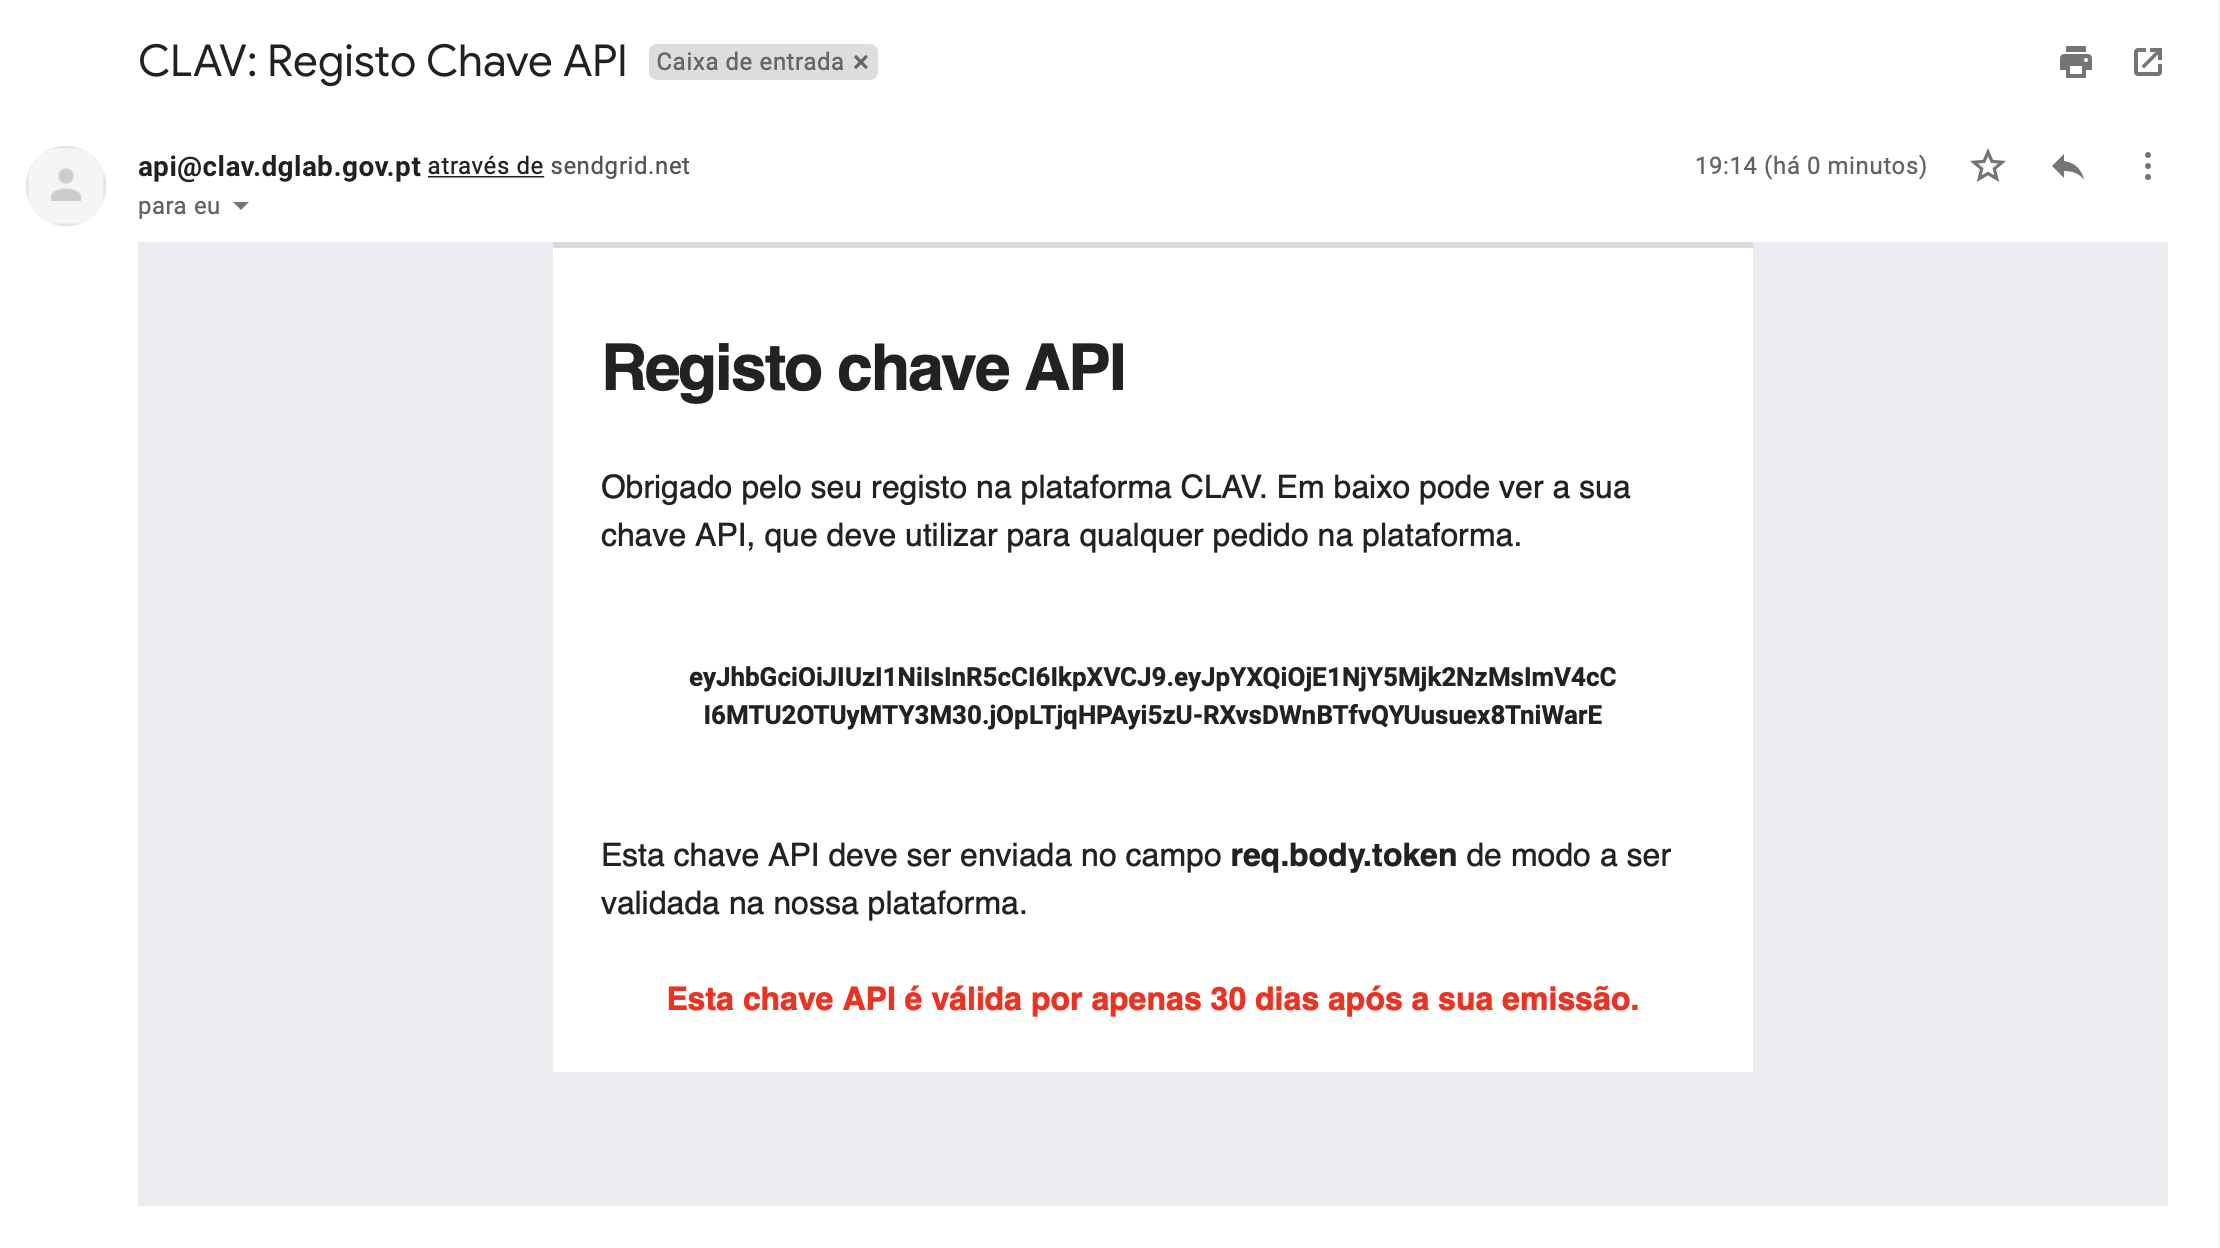
\includegraphics[width=0.95\textwidth]{img/clav/authAPI/emailRegisto.png}
    \caption{Email de registo contendo uma chave API da plataforma \gls{clav}.}
    \label{fig:emailRegistoChaveApi}
\end{figure}

Como podemos verificar na figura \ref{fig:emailRegistoChaveApi}, a chave API possui uma validade de 30 dias, após a qual é necessário renovar a mesma de modo a continuar a utilizar a API. Além disso, é enviada a chave em formato de um token \gls{jwt}, bem como a maneira correta de enviar o token para processamento pelo backend a cada pedido realizado.

\subsection{Renovação}

Como explicado na secção \ref{registoChaveApi}, a chave API apenas possui uma validade de 30 dias. Esta foi implementada de modo a diminuir potenciais abusos ou pedidos excessivos por parte de um fornecedor de serviços, bem como estudar a utilização da chave API, identificando a origem dos pedidos que mais tráfego geram, entre outras medidas.

\begin{figure}[H]
    \centering
    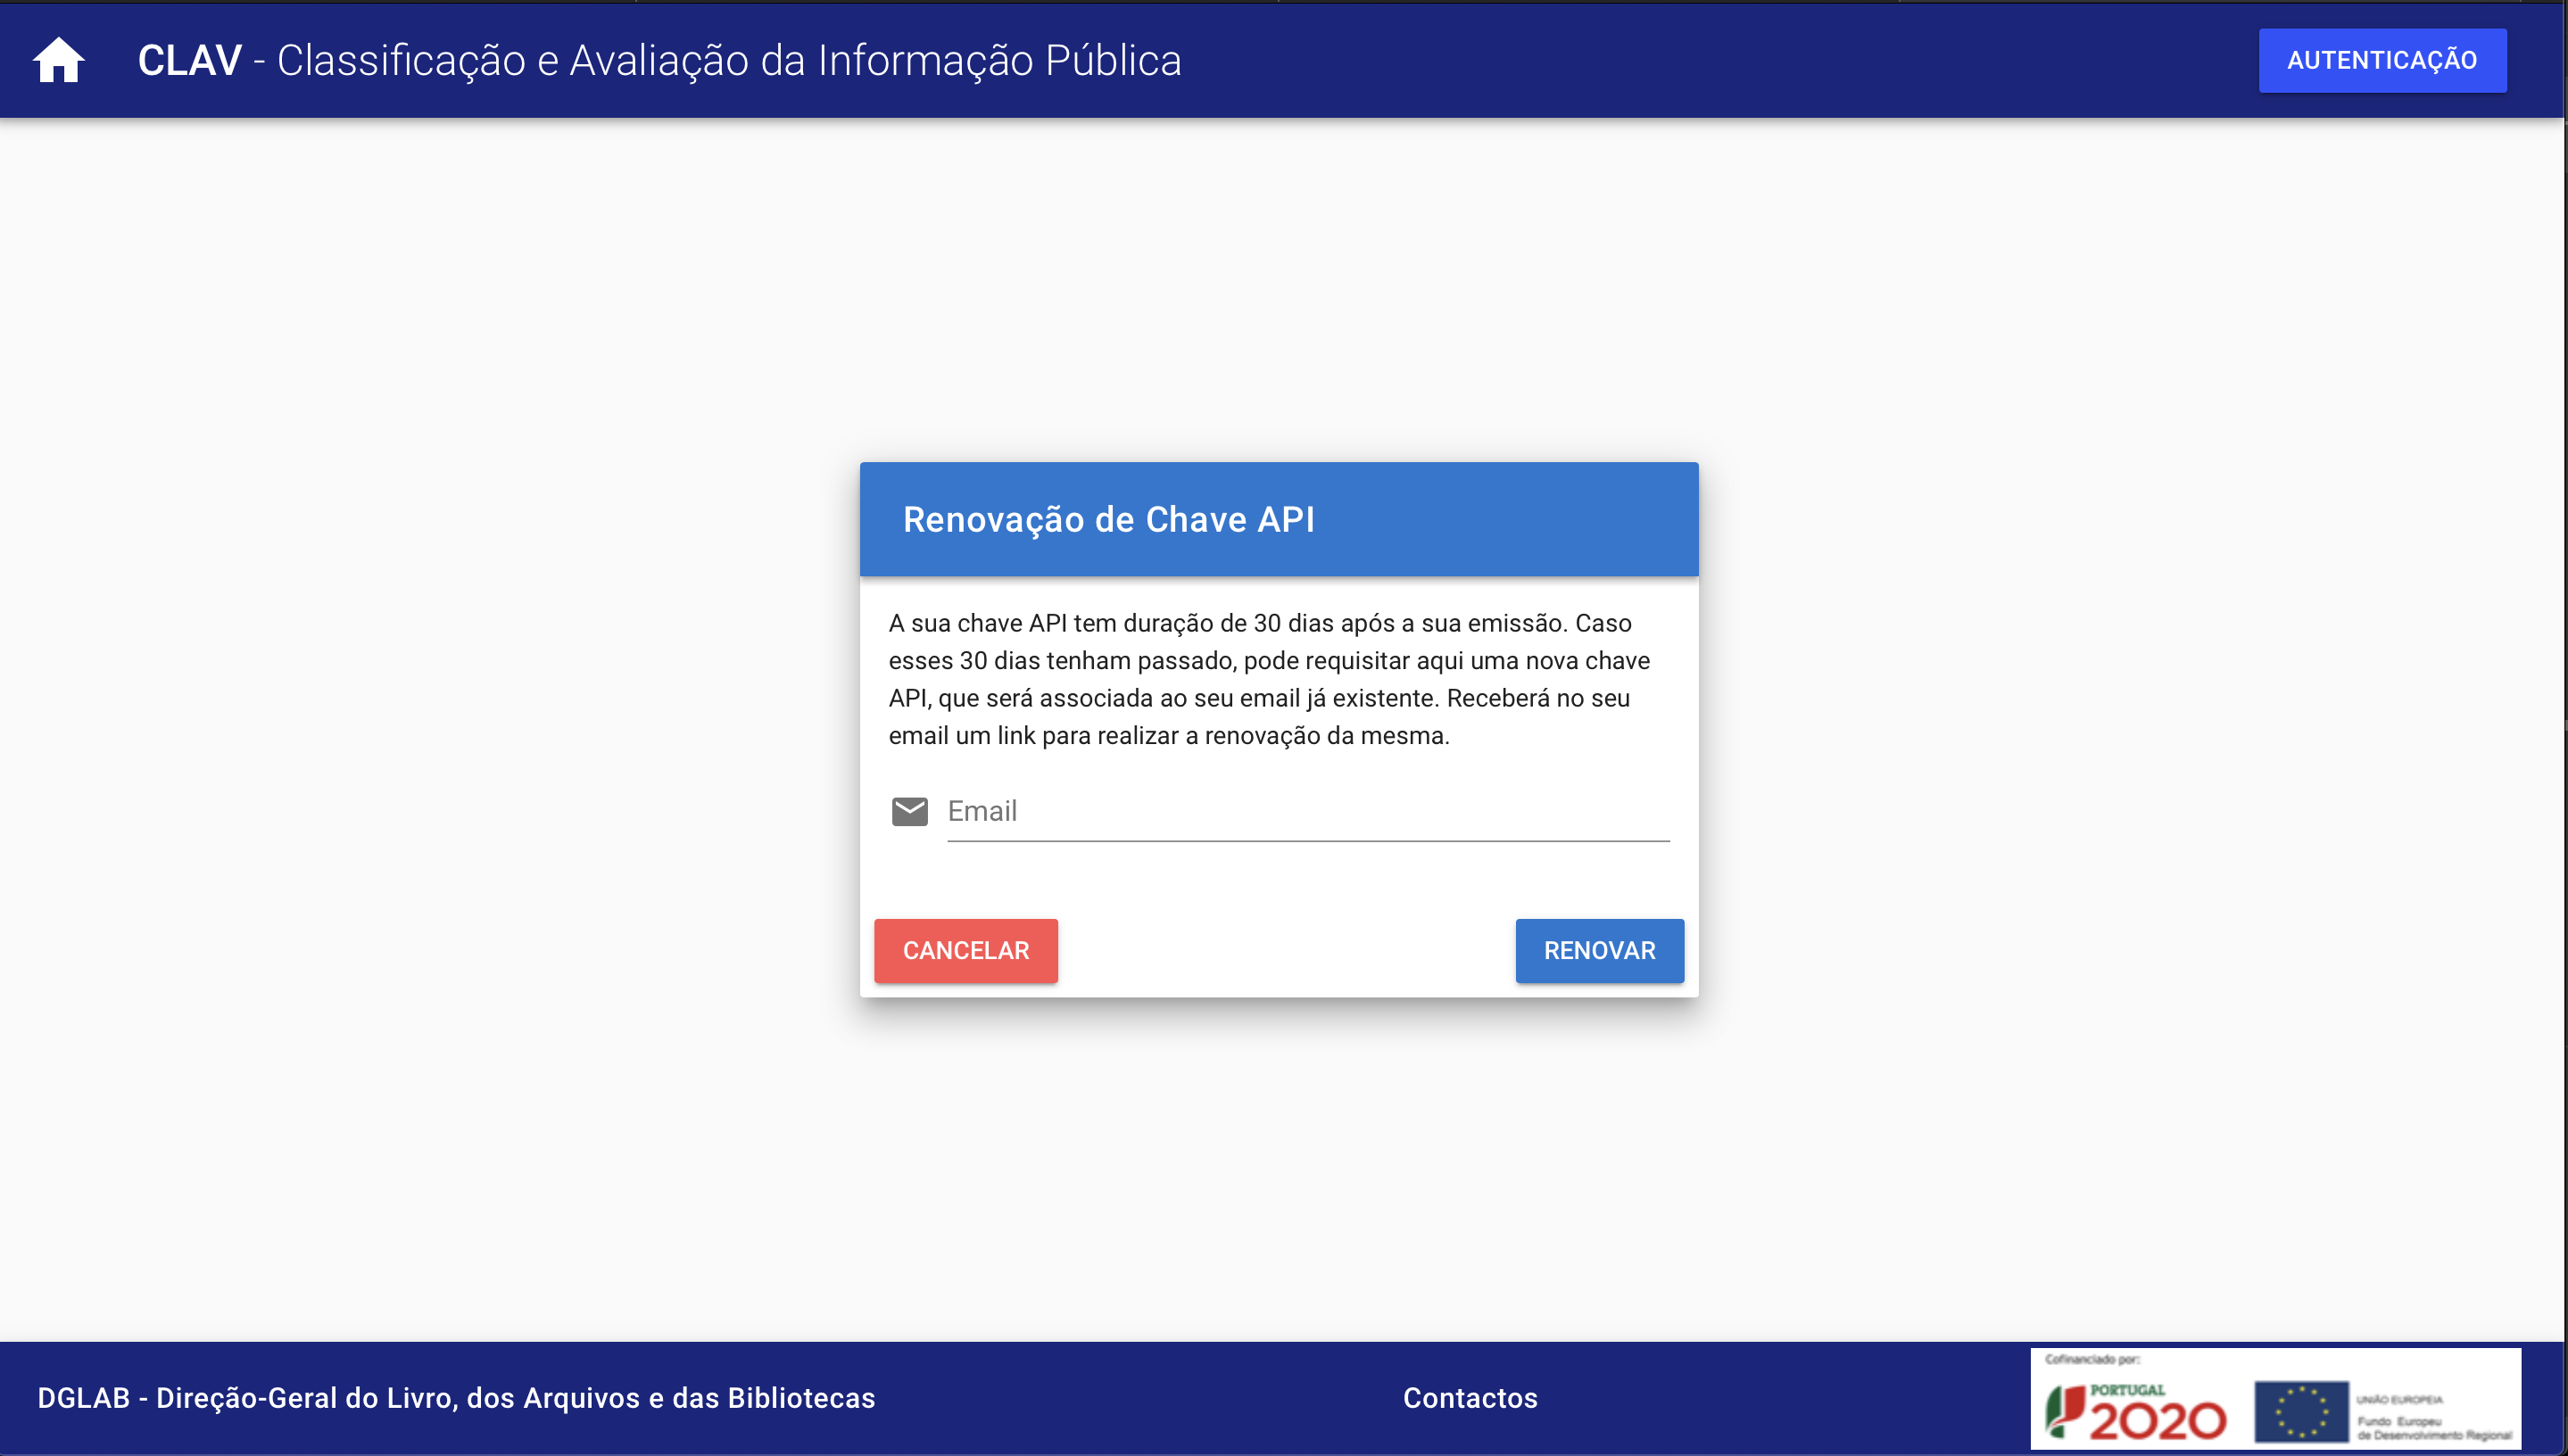
\includegraphics[width=0.95\textwidth]{img/clav/authAPI/renovar.png}
    \caption{Página de renovação de uma chave API na plataforma \gls{clav}.}
    \label{fig:renovarChaveAPI}
\end{figure}

De modo a renovar a chave API apenas é necessário introduzir o email utilizado para o registo da mesma, podendo ocorrer um de dois cenários:

\begin{itemize}
    \item \textbf{Sucesso}
    
    Ocorre quando o utilizador insere um email associado a uma chave API.
    
    \begin{figure}[H]
        \centering
        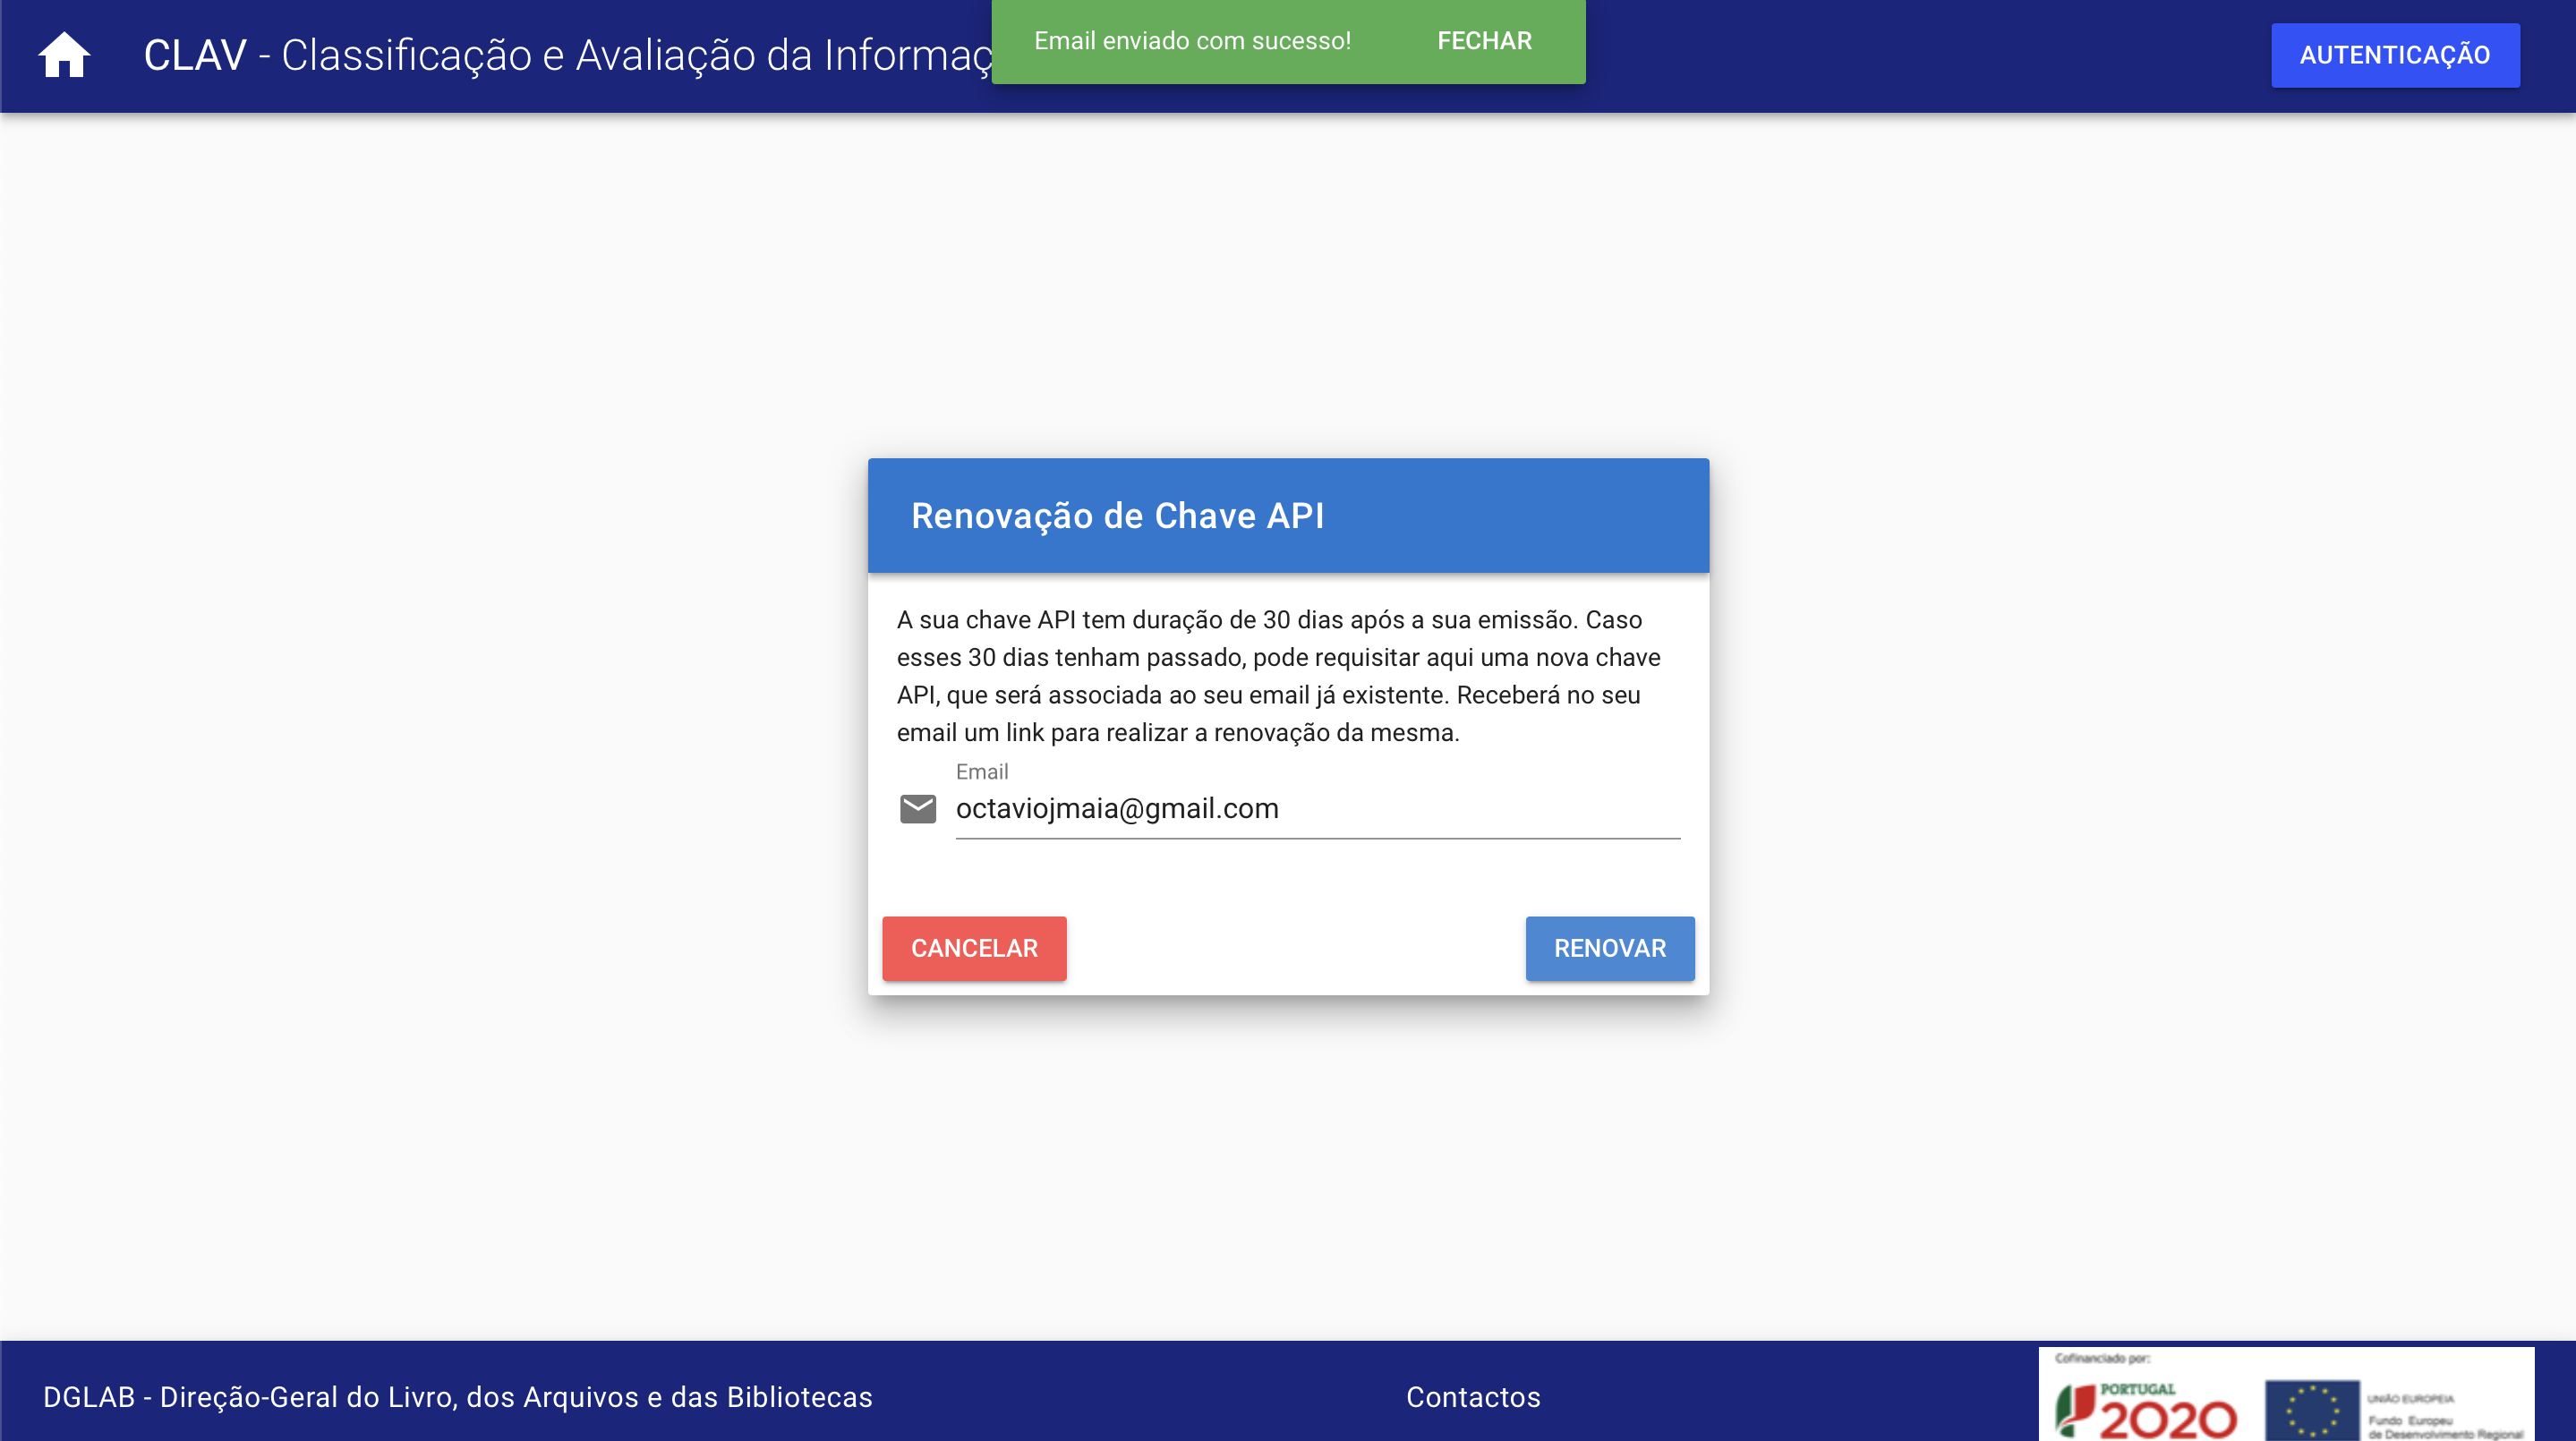
\includegraphics[width=0.95\textwidth]{img/clav/authAPI/sucessoRenovacao.png}
        \caption{Mensagem de sucesso após fornecer um email correto para renovação de uma chave API na plataforma \gls{clav}.}
        \label{fig:renovarChaveApiSucesso}
    \end{figure}
    
    Após ser introduzido um email correto é enviado um email contendo um URL para renovação da chave API em causa.
    
    \begin{figure}[H]
        \centering
        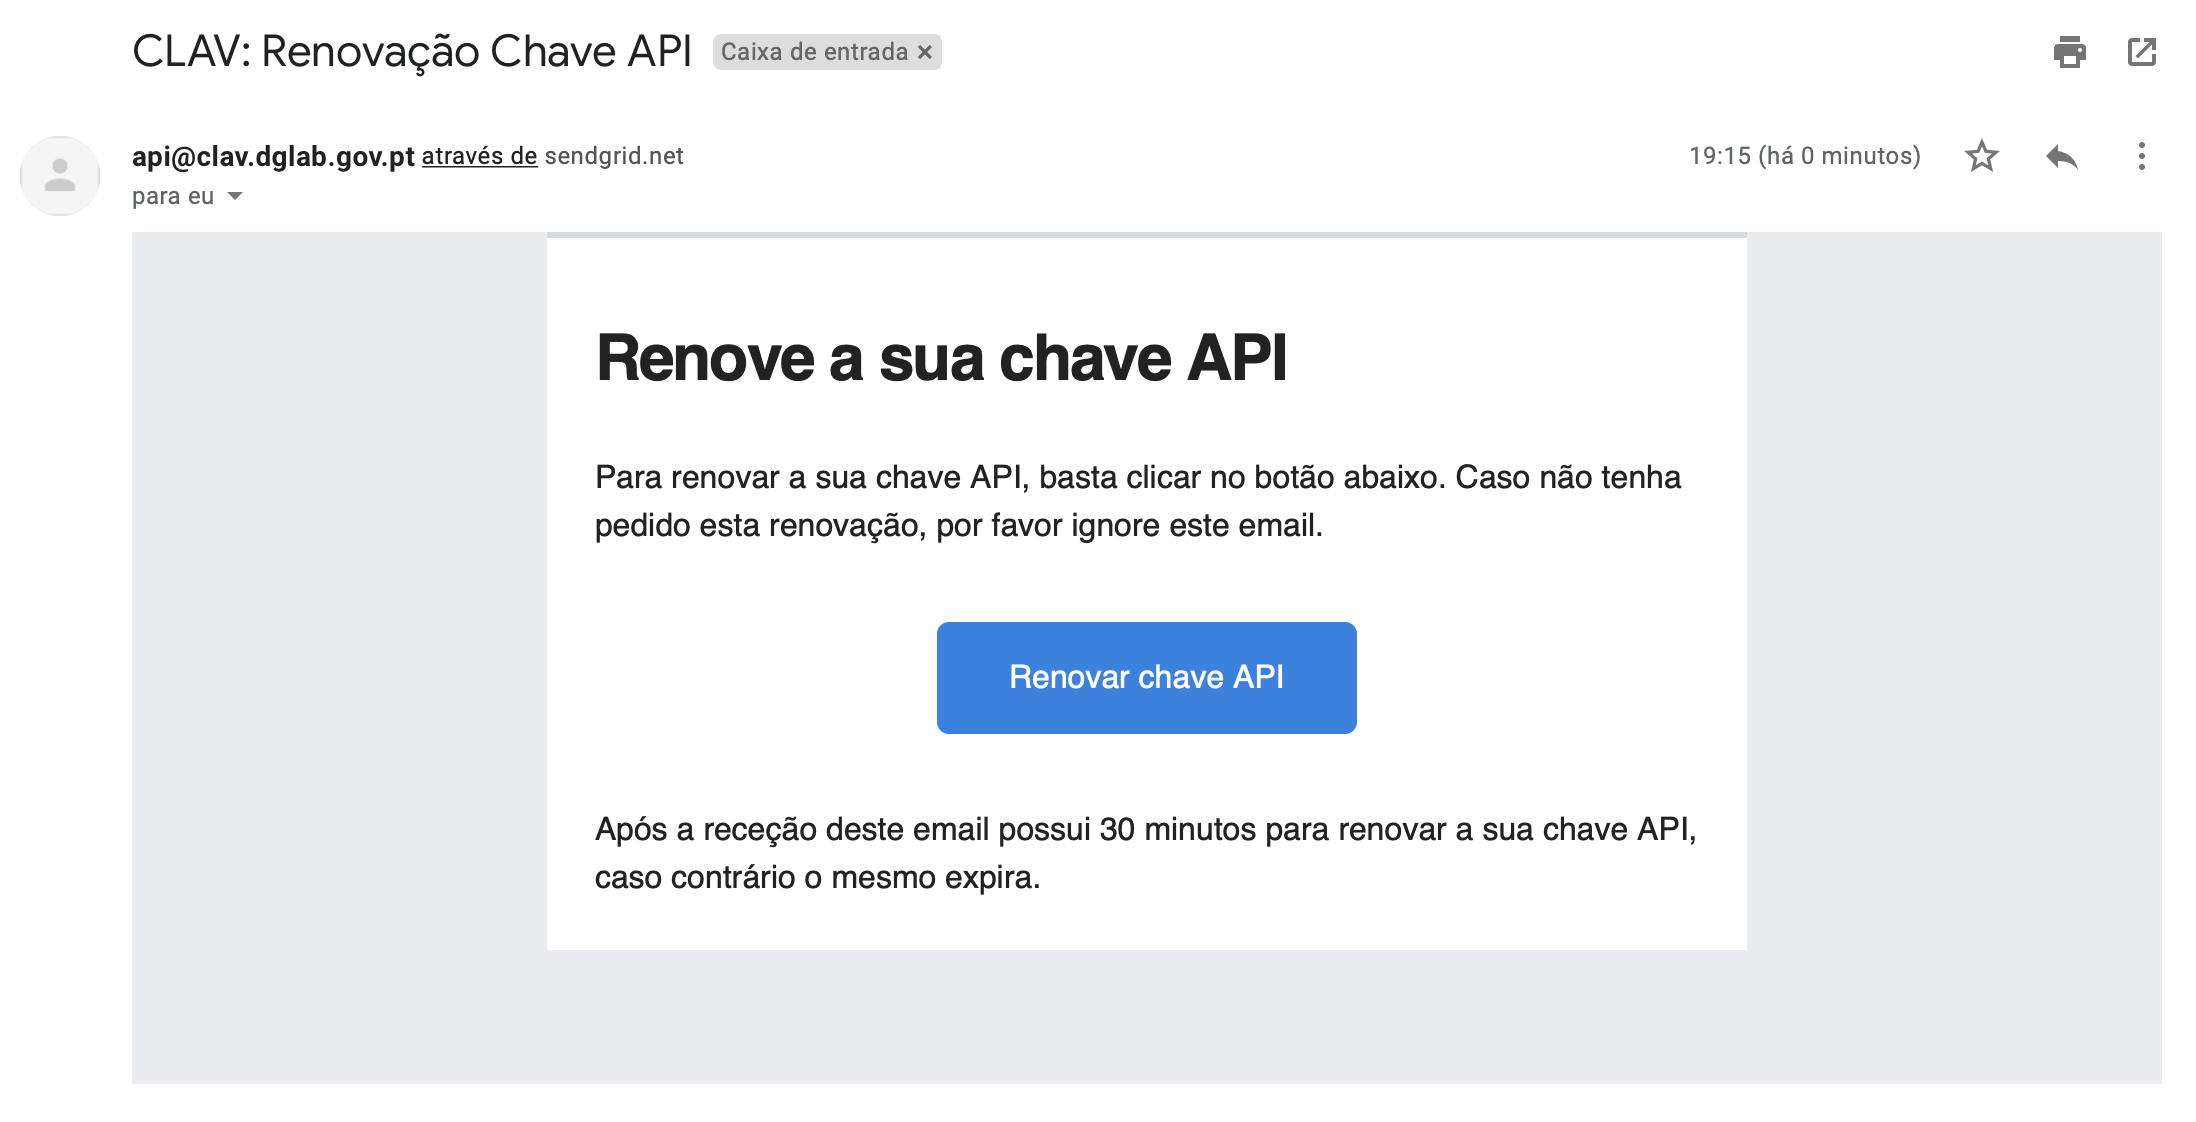
\includegraphics[width=0.95\textwidth]{img/clav/authAPI/emailRenovar.png}
        \caption{Email de renovação contendo a nova chave API da plataforma \gls{clav}.}
        \label{fig:emailRenovacaoChaveApi}
    \end{figure}
    
    Após recepção do email, basta aceder ao URL presente no email e será enviada uma nova chave API, sendo a chave anterior desativada.
    
    \begin{figure}[H]
        \centering
        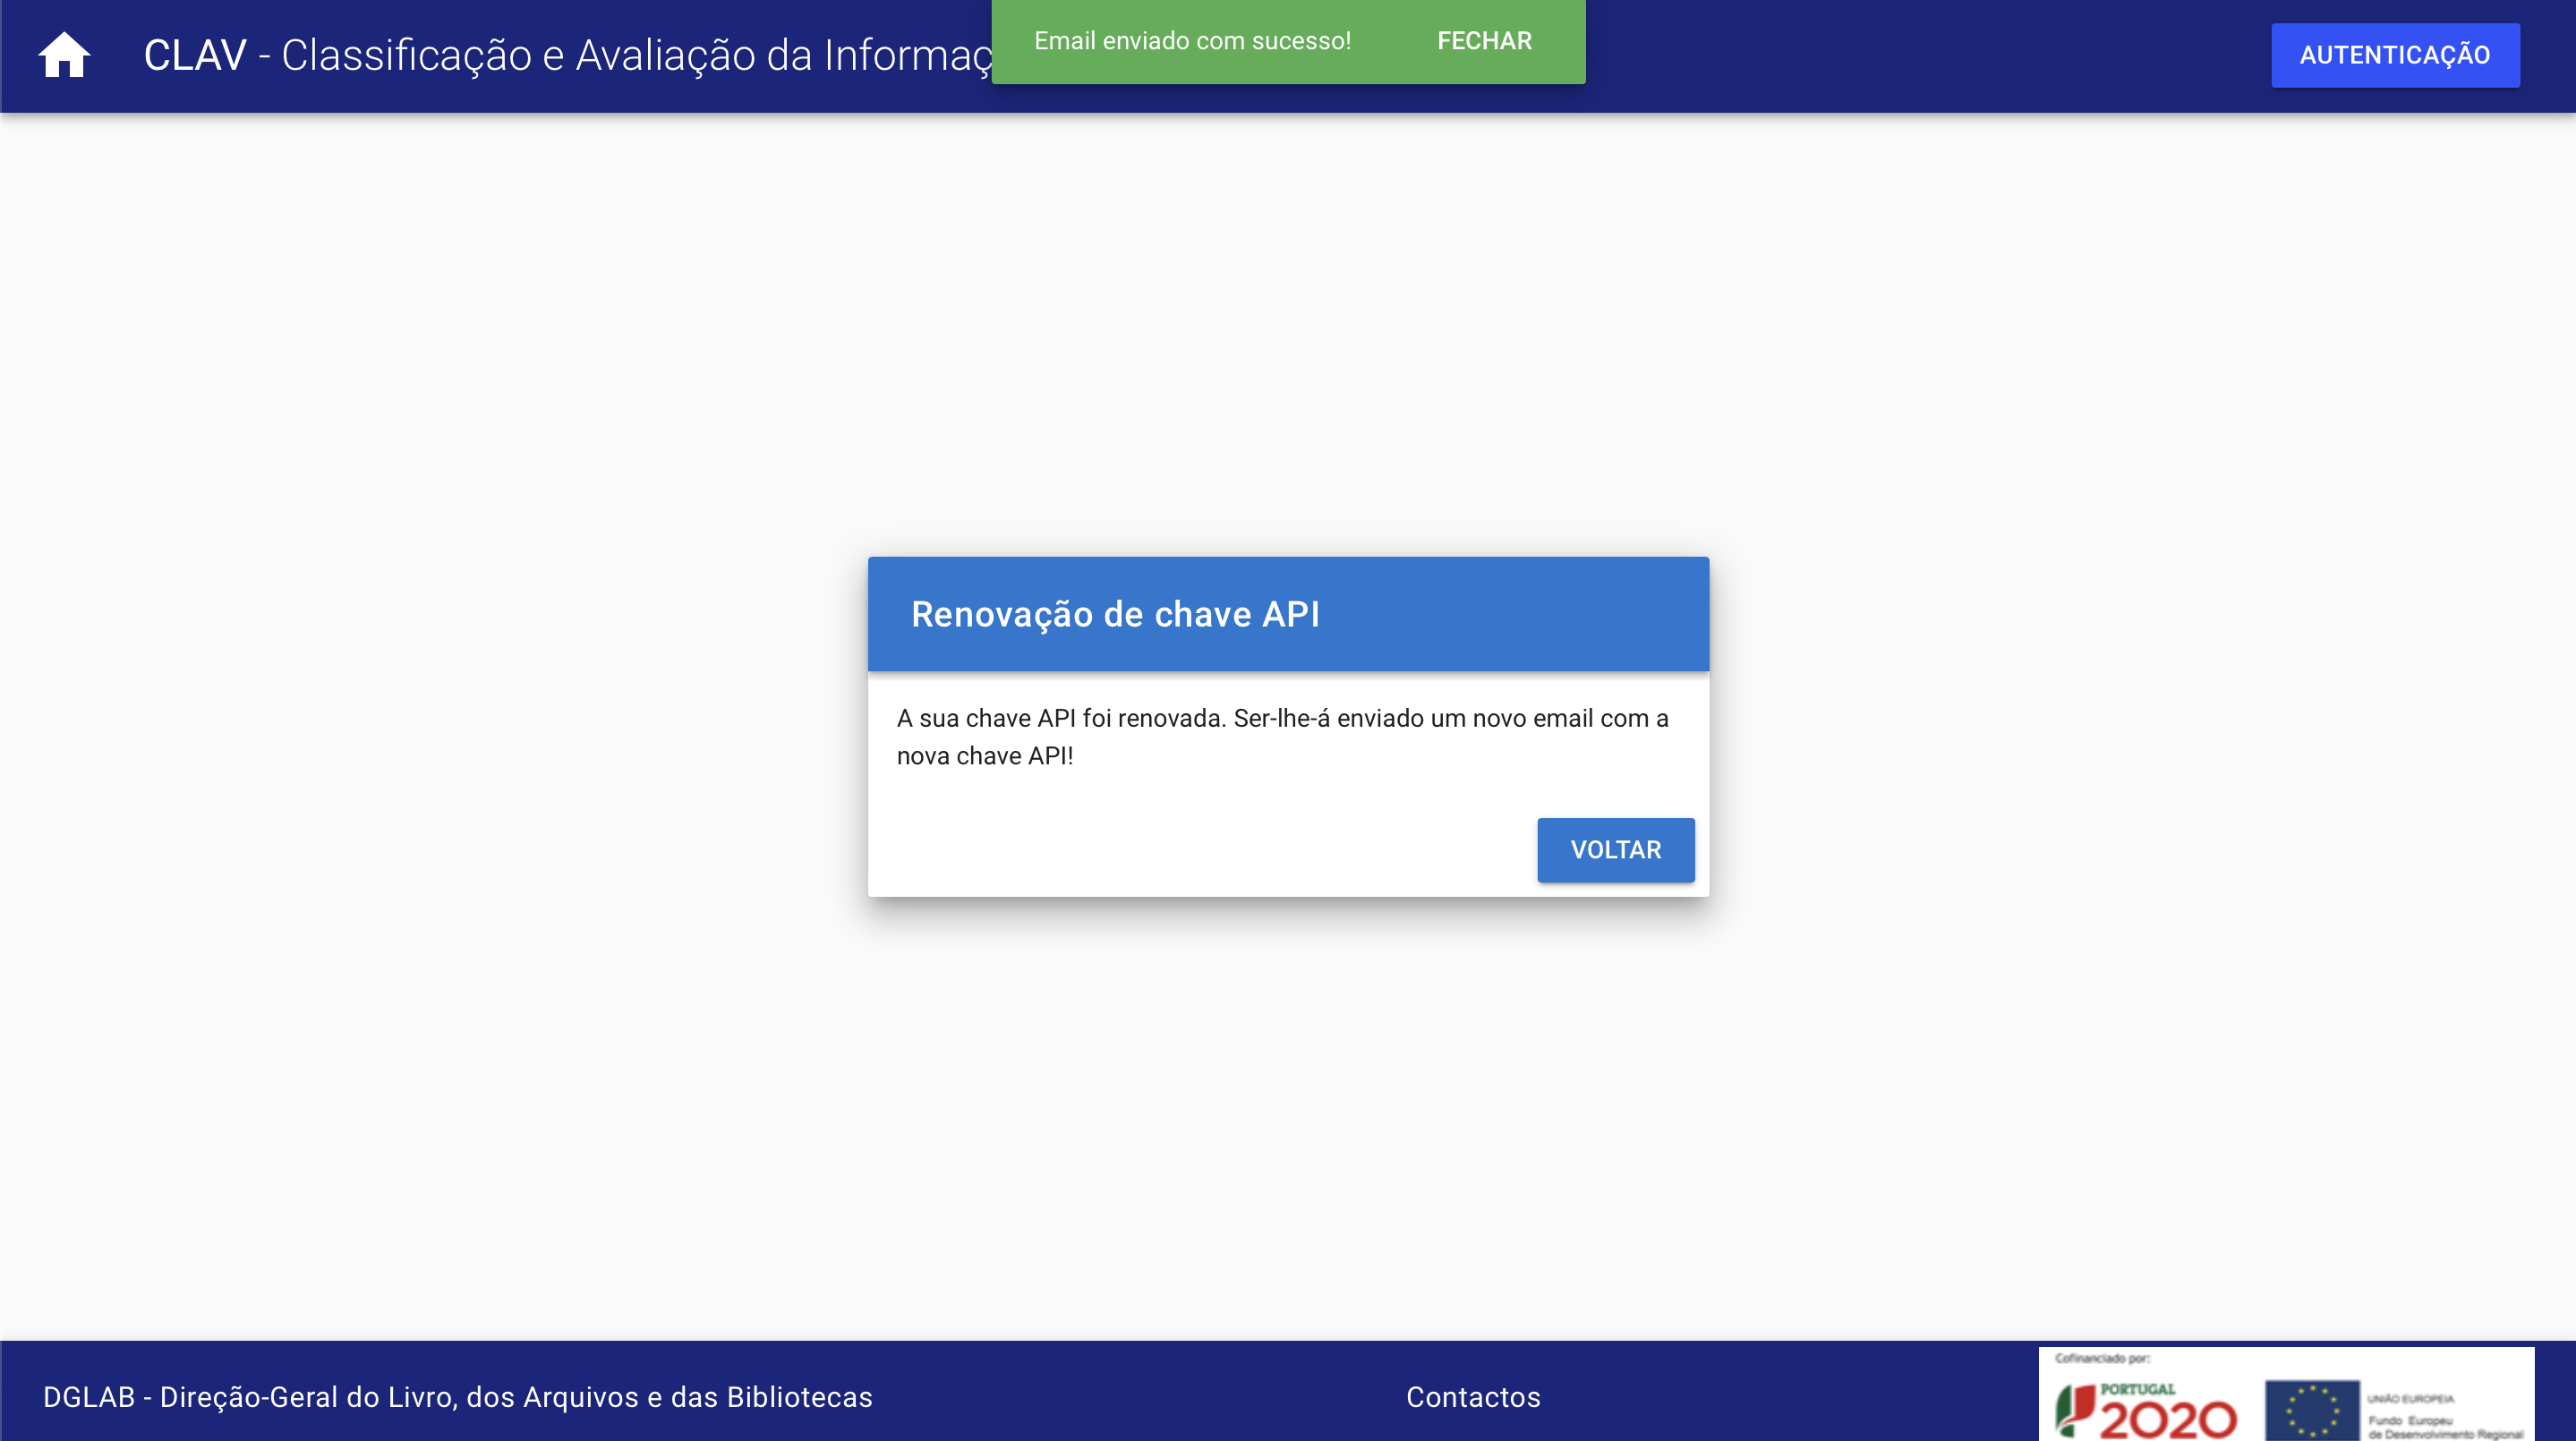
\includegraphics[width=0.95\textwidth]{img/clav/authAPI/sucessoRenovacao2.png}
        \caption{Mensagem de sucesso após clicar no link de renovação de uma chave API na plataforma \gls{clav}.}
        \label{fig:renovarChaveApiSucesso2}
    \end{figure}
    
    \begin{figure}[H]
        \centering
        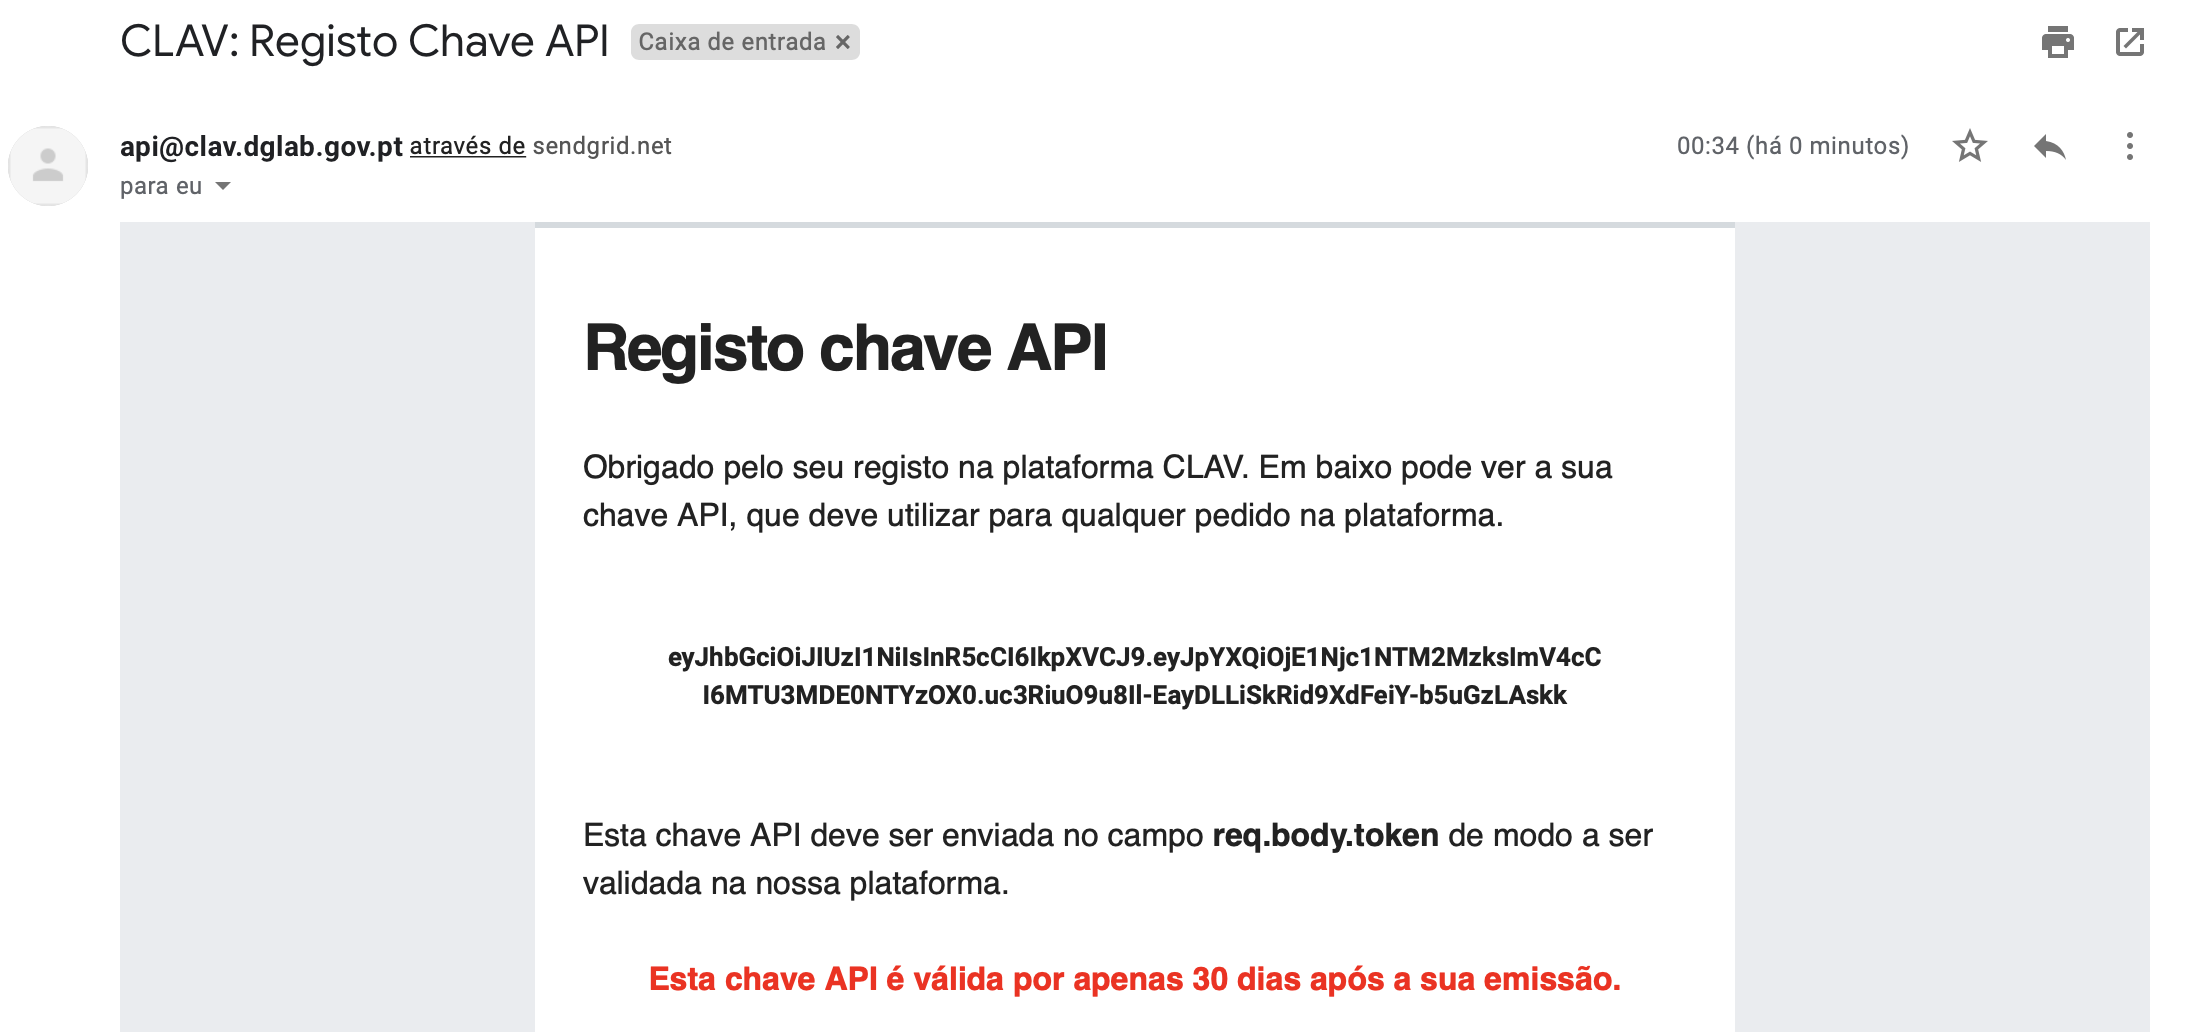
\includegraphics[width=0.95\textwidth]{img/clav/authAPI/emailNovaChave.png}
        \caption{Email de renovação contendo a nova chave API da plataforma \gls{clav}.}
        \label{fig:emailNovaChave}
    \end{figure}

    \item \textbf{Insucesso}
    
    Ocorre quando o utilizador fornece um email incorreto, ou seja, não associado a uma chave API.
    
    \begin{figure}[H]
        \centering
        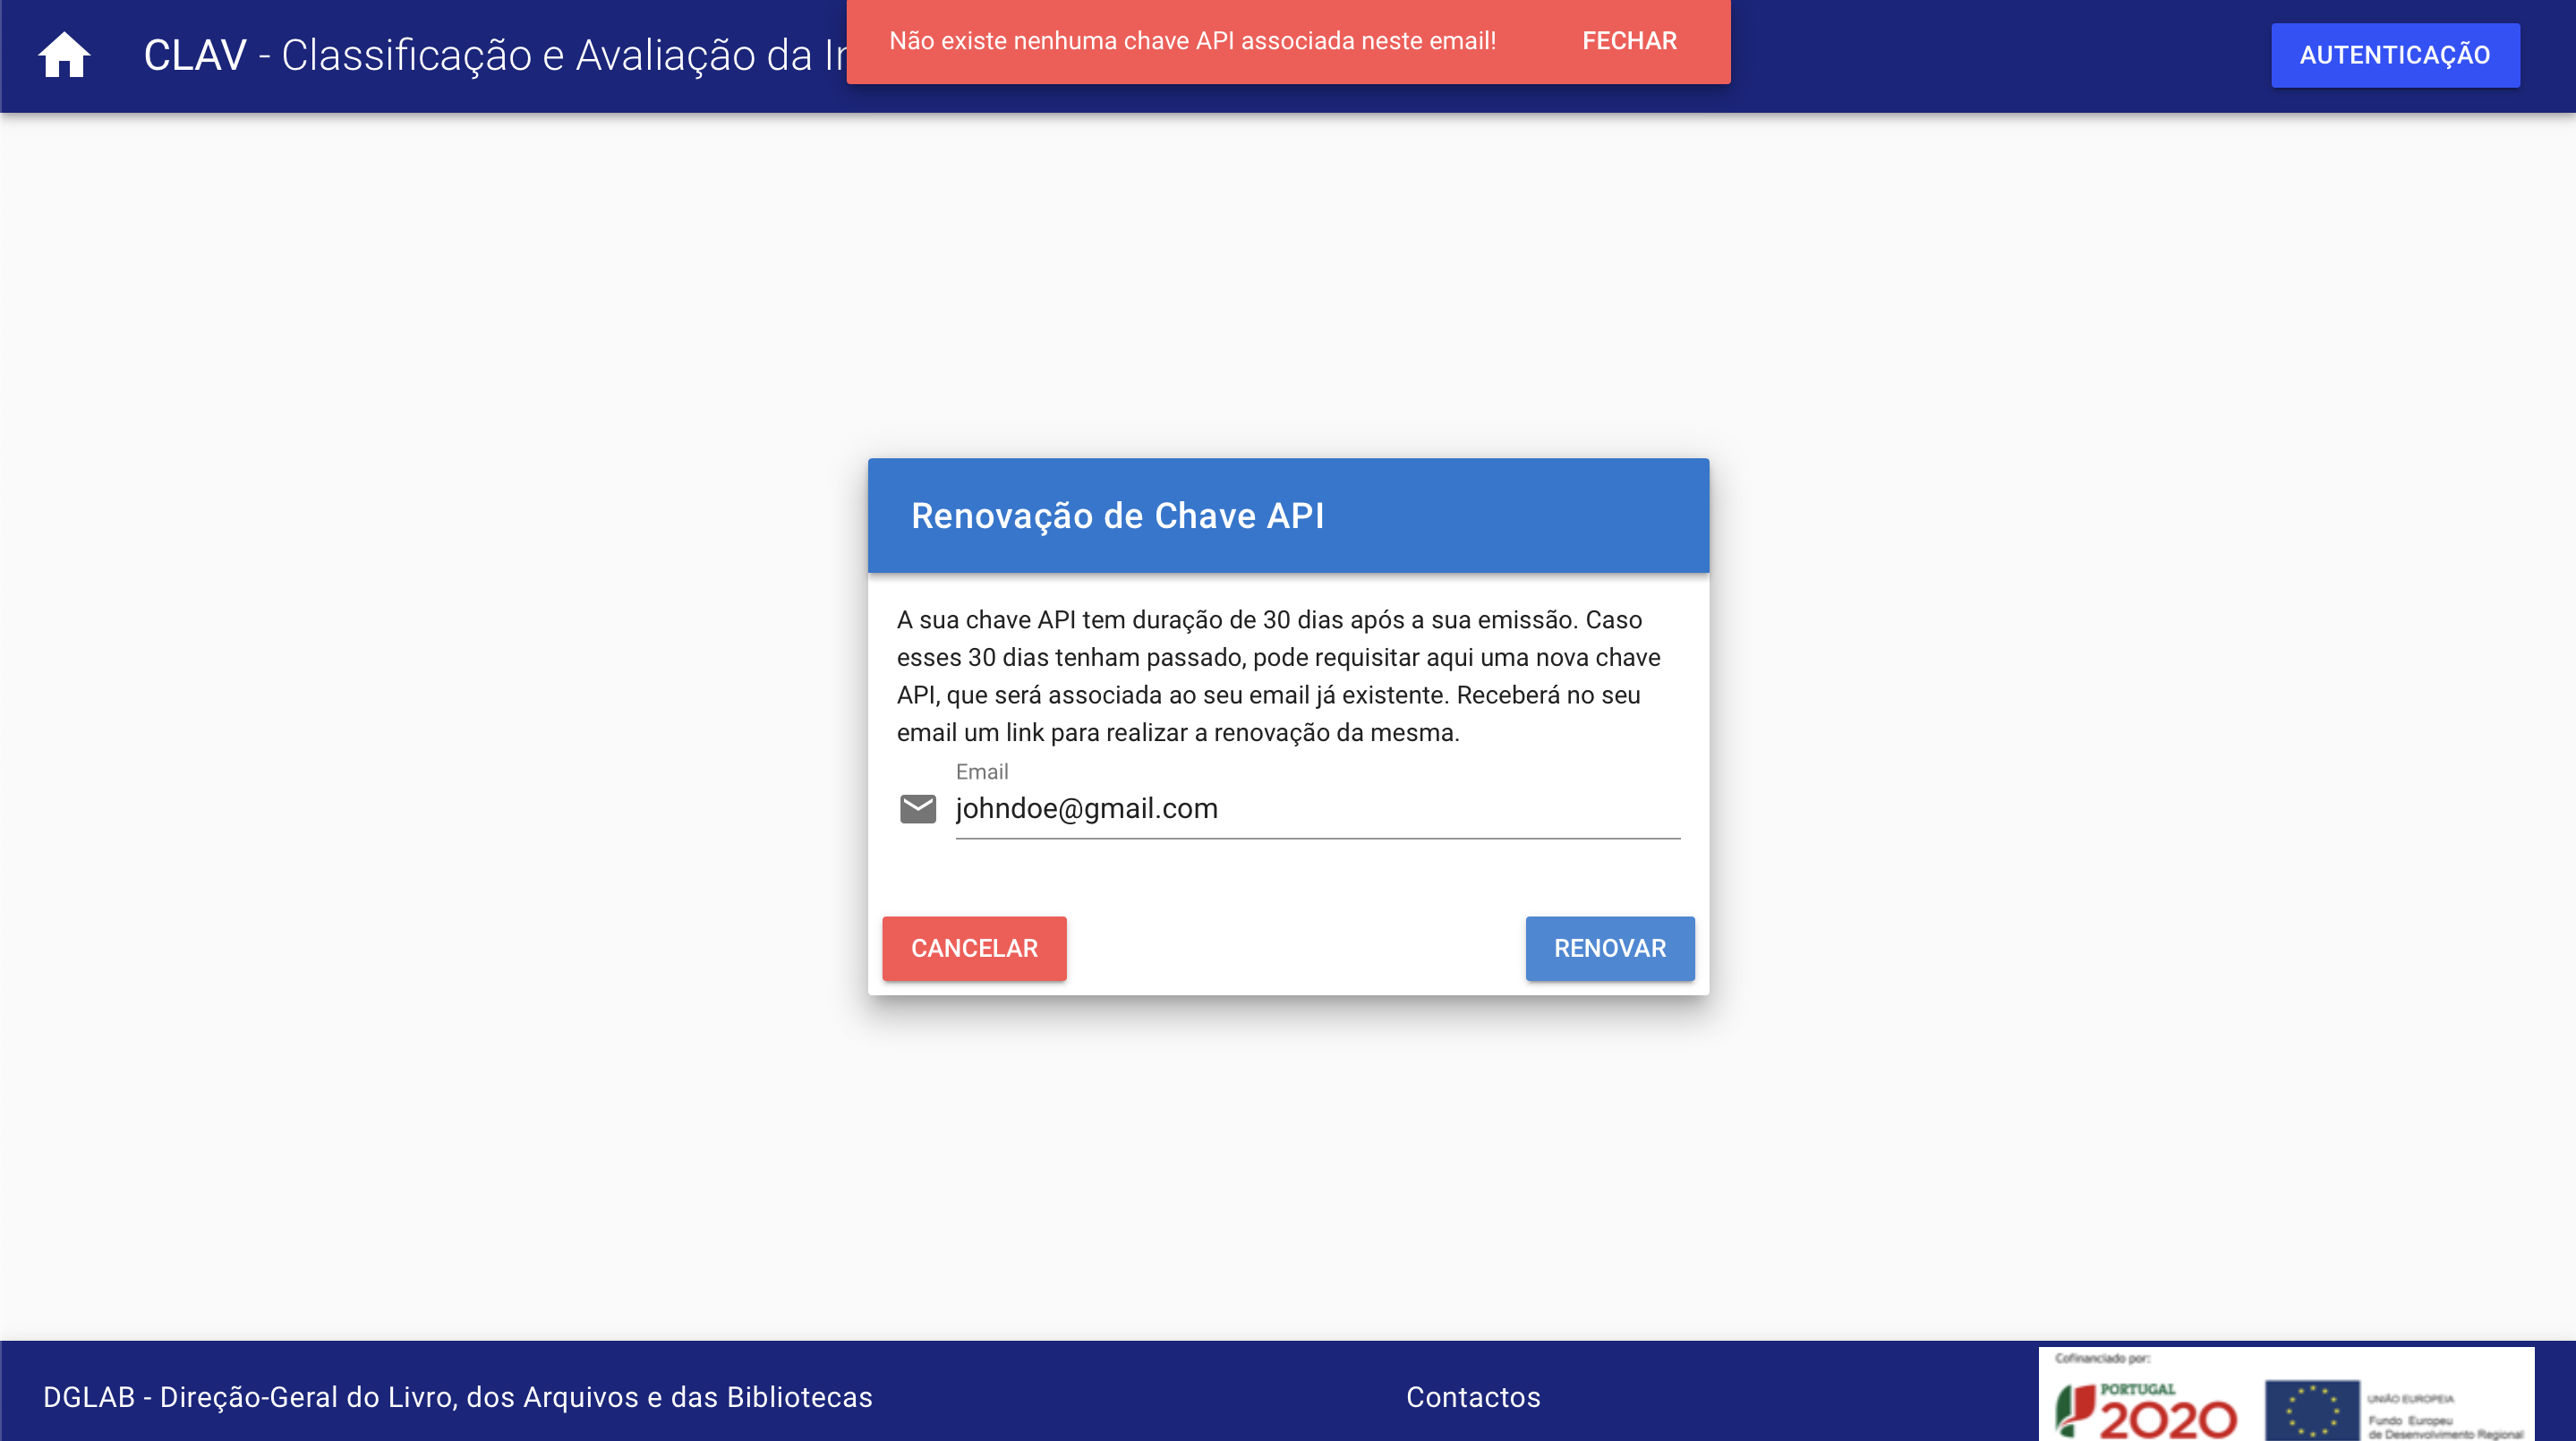
\includegraphics[width=0.95\textwidth]{img/clav/authAPI/erroRenovacao.png}
        \caption{Mensagem de erro após fornecer um email incorreto para renovação de uma chave API na plataforma \gls{clav}.}
        \label{fig:renovarChaveApiSucesso}
    \end{figure}
\end{itemize}

\cleardoublepage
O comportamento da função de registo da chave API pode ser exemplificado pelo seguinte diagrama de sequência:

\begin{figure}[H]
    \centering
    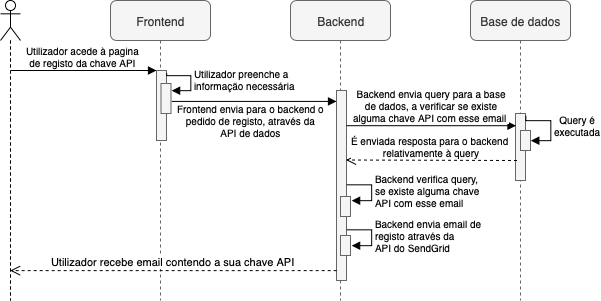
\includegraphics[width=0.87\textwidth]{img/diagramas/sequencia/DiagramasSequencia-RegistoAPI.png}
    \caption{Diagrama de sequência relativo ao processo de registo de uma chave API na plataforma \gls{clav}.}
    \label{fig:diagramaSequenciaRegistoAPI}
\end{figure}
\vspace{-5mm}
O comportamento da função de renovação da chave API pode ser exemplificado pelo seguinte diagrama de sequência:
\vspace{-2mm}
\begin{figure}[H]
    \centering
    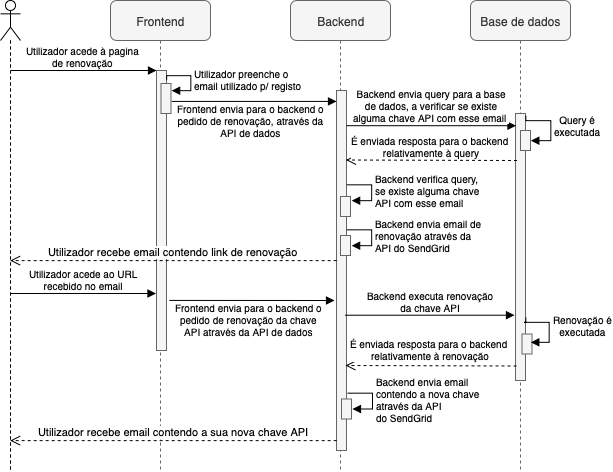
\includegraphics[width=0.87\textwidth]{img/diagramas/sequencia/DiagramasSequencia-RenovacaoAPI.png}
    \caption{Diagrama de sequência relativo ao processo de renovação de uma chave API na plataforma \gls{clav}.}
    \label{fig:diagramaSequenciaRenovacaoAPI}
\end{figure}

\cleardoublepage
\section{Gestão de utilizadores}

\cleardoublepage
\section{Autenticação backend}

De modo a proporcionar mecanismos capazes de lidar com os diversos tipos de utilizadores presentes na plataforma \gls{clav}, foi implementada uma solução baseada em \emph{middleware}. As funções de \emph{middleware} são responsáveis pela verificação do nível de acesso do utilizador. 

Para tal, foram desenvolvidas as seguintes funções, \emph{checkLevel} e \emph{isLevel}, sendo a primeira uma chamada à função auxiliar \emph{isLevel}.

\begin{algorithm}
    \caption{Pseudo código da função de middleware \emph{checkLevel}.}
    \begin{algorithmic}[1]
        \Function{checkLevel7}{user, next}
            \State \textbf{return} isLevel(7, user, next)
    \EndFunction
    \end{algorithmic}
\end{algorithm}

No pseudo código anterior podemos ver a implementação da função \emph{checkLevel7}, cujo objectivo é verificar se o utilizador possui acesso de nível 7, ou superior.

Esta função recorre a uma chamada à função \emph{isLevel}, sendo passado como parâmetro o nível de acesso a verificar.

\begin{algorithm}
    \caption{Pseudo código da função de middleware \emph{isLevel}.}
    \begin{algorithmic}[1]
    \Function{isLevel}{clearance, user, next}
        \If {$user.isAuthenticated$}
            \If {$user.level \geq clearance$}
                \State \textbf{return} next()
            \Else
                \State \textbf{return} redirect('back')
            \EndIf
        \Else
            \State \textbf{return} redirect('login')
        \EndIf
    \EndFunction
    \end{algorithmic}
\end{algorithm}

Com as estratégias de autenticação mencionadas anteriormente podemos assegurar uma correta implementação de níveis de acesso, não sendo possível a utilizadores aceder a conteúdo ao qual não possuem permissão.

\section{Métrica da plataforma CLAV}